\documentclass[11pt,letterpaper]{article}
\usepackage[margin=1in]{geometry}
\usepackage[T1]{fontenc}
\usepackage{lmodern}
\usepackage{microtype}
\usepackage{amsmath,amssymb,amsthm}
\usepackage{booktabs}
\usepackage{array}
\usepackage{tabularx}
\usepackage{longtable}
\usepackage{enumitem}
\usepackage{xcolor}
\usepackage{float}
\usepackage{graphicx}
\usepackage[skip=5pt,font=small]{caption}
\usepackage{pgfplots}
\pgfplotsset{compat=1.18}
\usepgfplotslibrary{groupplots}
\usepackage[colorlinks=true,linkcolor=black,citecolor=black,urlcolor=blue!50!black]{hyperref}
\setlist{itemsep=2pt,topsep=4pt}
\setlength{\emergencystretch}{3em}
\renewcommand{\topfraction}{0.9}
\renewcommand{\bottomfraction}{0.8}
\renewcommand{\floatpagefraction}{0.85}
\renewcommand{\textfraction}{0.08}
\setcounter{tocdepth}{1}
\newtheorem{proposition}{Proposition}
\newtheorem{lemma}{Lemma}
\newtheorem{corollary}{Corollary}
\newcommand{\E}{\mathbb{E}}
\newcommand{\V}{\mathbb{V}}
\newcommand{\Cov}{\mathbb{C}}
\newcommand{\Var}{\operatorname{Var}}
\newcommand{\tr}{\operatorname{tr}}
\newcommand{\diag}{\operatorname{diag}}
\newcommand{\st}{\tilde\sigma}
\newcommand{\op}{\mathrm{op}}
\newcommand{\cR}{\mathcal{R}}
\newcommand{\cG}{\mathcal{G}}
\newcommand{\bnu}{\bar\nu}
\newcommand{\bth}{\bar\vartheta}
\newcommand{\fevc}{\texorpdfstring{\texttt{fevc}}{fevc}}
\newcommand{\code}[1]{\texttt{#1}}
\newcommand{\pend}{\textit{stopped}}
\definecolor{cstay}{HTML}{0072B2}
\definecolor{cmove}{HTML}{D55E00}
\definecolor{cgrey}{HTML}{555555}
\makeatletter
\newcommand{\R}[1]{\ifcsname res@#1\endcsname\csname res@#1\endcsname\else\textbf{[\detokenize{#1}]}\fi}
\newcommand{\setres}[2]{\expandafter\gdef\csname res@#1\endcsname{#2}}
\newcommand{\tabinput}[1]{\@@input #1 }
\makeatother
\setres{real.theta.alpha}{0.0970}
\setres{real.se.alpha}{2.18}
\setres{real.relse.alpha}{0.22\%}
\setres{real.plugin.alpha}{0.1087}
\setres{real.theta.psi}{0.0261}
\setres{real.se.psi}{1.96}
\setres{real.relse.psi}{0.75\%}
\setres{real.plugin.psi}{0.0320}
\setres{real.theta.cov}{0.0134}
\setres{real.se.cov}{0.96}
\setres{real.relse.cov}{0.71\%}
\setres{real.plugin.cov}{0.0085}
\setres{real.theta.sum}{0.1499}
\setres{real.se.sum}{0.95}
\setres{real.relse.sum}{0.06\%}
\setres{real.plugin.sum}{0.1577}
\setres{real.rel_se_sum}{0.06\%}
\setres{real.relse.min}{0.06\%}
\setres{real.relse.max}{0.75\%}
\setres{real.run_maxdiff}{0.6\%}
\setres{real.se_solves}{260}
\setres{real.se_seconds}{131}
\setres{real.factor_minutes}{9}
\setres{real.probe_solves}{4{,}800}
\setres{real.floor.scale}{0.00\%}
\setres{real.floor.profile}{0.00\%}
\setres{real.floor.final}{0.00\%}
\setres{real.load.c0}{-1.12}
\setres{real.load.c1}{2.01}
\setres{real.profile_r2}{0.037}
\setres{real.capped.stayers}{2.5\%}
\setres{real.capped.movers}{1.0\%}
\setres{real.capped.first_term.sum}{26\%}
\setres{real.capped.first_term.max}{26\%}
\setres{real.coef.one}{0.81}
\setres{real.coef.a}{-0.33}
\setres{real.coef.aa}{0.22}
\setres{real.coef.p}{-0.08}
\setres{real.coef.pp}{0.02}
\setres{real.coef.ap}{-0.00}
\setres{real.share.movers.alpha}{97\%}
\setres{real.share.stayers.alpha}{3\%}
\setres{real.first_over_V.alpha}{110\%}
\setres{real.adjust_over_V.alpha}{-0.03\%}
\setres{real.share.movers.psi}{100\%}
\setres{real.share.stayers.psi}{0\%}
\setres{real.first_over_V.psi}{111\%}
\setres{real.adjust_over_V.psi}{0.00\%}
\setres{real.share.movers.cov}{100\%}
\setres{real.share.stayers.cov}{0\%}
\setres{real.first_over_V.cov}{141\%}
\setres{real.adjust_over_V.cov}{0.00\%}
\setres{real.share.movers.sum}{77\%}
\setres{real.share.stayers.sum}{23\%}
\setres{real.first_over_V.sum}{108\%}
\setres{real.adjust_over_V.sum}{-0.18\%}
\setres{real.adjust_max}{0.19\%}
\setres{real.max_stayer_share}{0.5\%}
\setres{real.max_mover_share}{1.9\%}
\setres{real.d2.min}{0.0006}
\setres{real.d2.max}{0.0070}
\setres{real.reff.min}{900}
\setres{real.reff.max}{4{,}600}
\setres{real.lambda.min}{0.0004}
\setres{real.lambda.max}{0.0024}
\setres{real.n.rows}{4{,}063{,}732}
\setres{real.n.mover_rows}{1{,}034{,}376}
\setres{real.n.stayer_rows}{3{,}029{,}356}
\setres{real.n.person_years}{5{,}163{,}428}
\setres{real.n.firms}{86{,}647}
\setres{real.n.workers}{1{,}106{,}419}
\setres{real.n.stayers}{666{,}090}
\setres{real.n.movers}{440{,}329}
\setres{real.share.stayer_rows}{75\%}
\setres{real.share.stayer_py}{59\%}
\setres{real.within_match_mean}{0.013}
\setres{real.stayers_mean}{0.015}
\setres{real.within_match_matches}{560{,}235}
\setres{real.lo.len1}{0.043}
\setres{real.lo.longer.min}{0.055}
\setres{real.lo.longer.max}{0.057}
\setres{real.prof.alpha.stay.lo}{2.68}
\setres{real.prof.alpha.stay.hi}{1.18}
\setres{real.prof.alpha.stay.mid}{0.67}
\setres{real.prof.alpha.fit.lo}{2.25}
\setres{real.prof.alpha.fit.hi}{1.06}
\setres{real.prof.alpha.fit.mid}{0.83}
\setres{real.prof.alpha.move.lo}{2.42}
\setres{real.prof.alpha.move.hi}{1.08}
\setres{real.prof.alpha.move.mid}{0.76}
\setres{real.prof.psi.stay.lo}{1.35}
\setres{real.prof.psi.stay.hi}{0.91}
\setres{real.prof.psi.stay.mid}{0.97}
\setres{real.prof.psi.fit.lo}{1.32}
\setres{real.prof.psi.fit.hi}{0.89}
\setres{real.prof.psi.fit.mid}{0.98}
\setres{real.prof.psi.move.lo}{1.45}
\setres{real.prof.psi.move.hi}{1.12}
\setres{real.prof.psi.move.mid}{0.89}
\setres{dec.N1.gap.max}{14\%}
\setres{dec.N1.fit.maxgap}{17\%}
\setres{dec.N1.fit.bottom}{+13\%}
\setres{dec.N1.fit.mid}{-4\%}
\setres{dec.N1.fit.top}{+17\%}
\setres{dec.N6.gap.max}{9\%}
\setres{dec.N6.fit.maxgap}{27\%}
\setres{dec.N6.fit.bottom}{-2\%}
\setres{dec.N6.fit.mid}{-1\%}
\setres{dec.N6.fit.top}{+20\%}
\setres{dec.N10.gap.max}{10\%}
\setres{dec.N10.fit.maxgap}{29\%}
\setres{dec.N10.fit.bottom}{-0\%}
\setres{dec.N10.fit.mid}{-5\%}
\setres{dec.N10.fit.top}{+20\%}
\setres{dec.data.lo.bottom}{3.6}
\setres{dec.data.lo.mid}{0.56}
\setres{dec.data.lo.top}{1.9}
\setres{dec.data.fit.bottom}{-11\%}
\setres{dec.data.fit.mid}{+2\%}
\setres{dec.data.fit.top}{+10\%}
\setres{dec.data.fit.maxgap}{39\%}
\setres{dec.reps}{3}
\setres{dec.data.over.min}{13\%}
\setres{dec.data.over.max}{24\%}
\setres{dec.data.under.min}{16\%}
\setres{dec.data.under.max}{39\%}
\setres{dec.data.top}{+10\%}
\setres{dec.data.bottom}{-11\%}
\setres{dec.data.d1.lo}{17.9}
\setres{dec.data.d1.fit}{16.0}
\setres{dec.rows.min}{5\%}
\setres{dec.rows.max}{14\%}
\setres{dec.sim.gap.max}{14\%}
\setres{dec.sd.max}{4\%}
\setres{real.load.pibar}{1.06}
\setres{ctrl.sum}{7\%}
\setres{ctrl.others}{0.6\%}
\setres{ctrl.n.py}{5.25}
\setres{sim.all.min}{0.96}
\setres{sim.all.max}{1.10}
\setres{sim.all.cov.min}{0.935}
\setres{sim.all.cov.max}{0.980}
\setres{sim.all.or.min}{0.97}
\setres{sim.all.or.max}{1.03}
\setres{sim.a4.min}{0.96}
\setres{sim.a4.max}{1.10}
\setres{sim.a4.cov.min}{0.935}
\setres{sim.a4.cov.max}{0.980}
\setres{sim.a4.or.min}{0.97}
\setres{sim.a4.or.max}{1.03}
\setres{sim.norm.min}{0.98}
\setres{sim.norm.max}{1.10}
\setres{sim.norm.cov.min}{0.935}
\setres{sim.norm.cov.max}{0.980}
\setres{sim.norm.or.min}{1.00}
\setres{sim.norm.or.max}{1.01}
\setres{sim.shape.min}{0.96}
\setres{sim.shape.max}{1.09}
\setres{sim.shape.cov.min}{0.935}
\setres{sim.shape.cov.max}{0.980}
\setres{sim.shape.or.min}{0.97}
\setres{sim.shape.or.max}{1.03}
\setres{sim.viol.min}{0.97}
\setres{sim.viol.max}{1.10}
\setres{sim.viol.cov.min}{0.935}
\setres{sim.viol.cov.max}{0.975}
\setres{sim.viol.or.min}{1.00}
\setres{sim.viol.or.max}{1.00}
\setres{sim.short.N1.alpha}{-1\%}
\setres{sim.N1.alpha}{1.01}
\setres{sim.N1.cover.alpha}{0.94}
\setres{sim.N1.or.alpha}{1.00}
\setres{sim.short.N1.psi}{-0\%}
\setres{sim.N1.psi}{1.00}
\setres{sim.N1.cover.psi}{0.94}
\setres{sim.N1.or.psi}{1.00}
\setres{sim.short.N1.cov}{-0\%}
\setres{sim.N1.cov}{1.00}
\setres{sim.N1.cover.cov}{0.94}
\setres{sim.N1.or.cov}{1.00}
\setres{sim.short.N1.sum}{-6\%}
\setres{sim.N1.sum}{1.06}
\setres{sim.N1.cover.sum}{0.97}
\setres{sim.N1.or.sum}{1.00}
\setres{sim.short.N2.alpha}{-5\%}
\setres{sim.N2.alpha}{1.05}
\setres{sim.N2.cover.alpha}{0.97}
\setres{sim.N2.or.alpha}{1.00}
\setres{sim.short.N2.psi}{-10\%}
\setres{sim.N2.psi}{1.10}
\setres{sim.N2.cover.psi}{0.95}
\setres{sim.N2.or.psi}{1.00}
\setres{sim.short.N2.cov}{-3\%}
\setres{sim.N2.cov}{1.03}
\setres{sim.N2.cover.cov}{0.96}
\setres{sim.N2.or.cov}{1.01}
\setres{sim.short.N2.sum}{0\%}
\setres{sim.N2.sum}{1.00}
\setres{sim.N2.cover.sum}{0.96}
\setres{sim.N2.or.sum}{1.00}
\setres{sim.short.N3.alpha}{-6\%}
\setres{sim.N3.alpha}{1.06}
\setres{sim.N3.cover.alpha}{0.97}
\setres{sim.N3.or.alpha}{1.00}
\setres{sim.short.N3.psi}{-9\%}
\setres{sim.N3.psi}{1.09}
\setres{sim.N3.cover.psi}{0.98}
\setres{sim.N3.or.psi}{1.00}
\setres{sim.short.N3.cov}{-6\%}
\setres{sim.N3.cov}{1.06}
\setres{sim.N3.cover.cov}{0.98}
\setres{sim.N3.or.cov}{1.00}
\setres{sim.short.N3.sum}{-3\%}
\setres{sim.N3.sum}{1.03}
\setres{sim.N3.cover.sum}{0.96}
\setres{sim.N3.or.sum}{1.01}
\setres{sim.short.N4.alpha}{-0\%}
\setres{sim.N4.alpha}{1.00}
\setres{sim.N4.cover.alpha}{0.96}
\setres{sim.N4.or.alpha}{0.99}
\setres{sim.short.N4.psi}{-7\%}
\setres{sim.N4.psi}{1.07}
\setres{sim.N4.cover.psi}{0.95}
\setres{sim.N4.or.psi}{1.00}
\setres{sim.short.N4.cov}{2\%}
\setres{sim.N4.cov}{0.98}
\setres{sim.N4.cover.cov}{0.95}
\setres{sim.N4.or.cov}{1.00}
\setres{sim.short.N4.sum}{4\%}
\setres{sim.N4.sum}{0.96}
\setres{sim.N4.cover.sum}{0.94}
\setres{sim.N4.or.sum}{0.97}
\setres{sim.short.N5.alpha}{-2\%}
\setres{sim.N5.alpha}{1.02}
\setres{sim.N5.cover.alpha}{0.95}
\setres{sim.N5.or.alpha}{1.01}
\setres{sim.short.N5.psi}{-7\%}
\setres{sim.N5.psi}{1.07}
\setres{sim.N5.cover.psi}{0.94}
\setres{sim.N5.or.psi}{1.00}
\setres{sim.short.N5.cov}{2\%}
\setres{sim.N5.cov}{0.98}
\setres{sim.N5.cover.cov}{0.97}
\setres{sim.N5.or.cov}{1.00}
\setres{sim.short.N5.sum}{-3\%}
\setres{sim.N5.sum}{1.03}
\setres{sim.N5.cover.sum}{0.96}
\setres{sim.N5.or.sum}{1.03}
\setres{sim.short.N6.alpha}{-6\%}
\setres{sim.N6.alpha}{1.06}
\setres{sim.N6.cover.alpha}{0.95}
\setres{sim.N6.or.alpha}{1.00}
\setres{sim.short.N6.psi}{-10\%}
\setres{sim.N6.psi}{1.10}
\setres{sim.N6.cover.psi}{0.97}
\setres{sim.N6.or.psi}{1.00}
\setres{sim.short.N6.cov}{-5\%}
\setres{sim.N6.cov}{1.05}
\setres{sim.N6.cover.cov}{0.98}
\setres{sim.N6.or.cov}{1.00}
\setres{sim.short.N6.sum}{-10\%}
\setres{sim.N6.sum}{1.10}
\setres{sim.N6.cover.sum}{0.96}
\setres{sim.N6.or.sum}{1.00}
\setres{sim.short.N7.alpha}{-2\%}
\setres{sim.N7.alpha}{1.02}
\setres{sim.N7.cover.alpha}{0.97}
\setres{sim.N7.or.alpha}{1.00}
\setres{sim.short.N7.psi}{-1\%}
\setres{sim.N7.psi}{1.01}
\setres{sim.N7.cover.psi}{0.95}
\setres{sim.N7.or.psi}{1.00}
\setres{sim.short.N7.cov}{2\%}
\setres{sim.N7.cov}{0.98}
\setres{sim.N7.cover.cov}{0.97}
\setres{sim.N7.or.cov}{1.00}
\setres{sim.short.N7.sum}{-2\%}
\setres{sim.N7.sum}{1.02}
\setres{sim.N7.cover.sum}{0.96}
\setres{sim.N7.or.sum}{1.00}
\setres{sim.short.N8.alpha}{-1\%}
\setres{sim.N8.alpha}{1.01}
\setres{sim.N8.cover.alpha}{0.94}
\setres{sim.N8.or.alpha}{1.00}
\setres{sim.short.N8.psi}{-8\%}
\setres{sim.N8.psi}{1.08}
\setres{sim.N8.cover.psi}{0.95}
\setres{sim.N8.or.psi}{1.00}
\setres{sim.short.N8.cov}{2\%}
\setres{sim.N8.cov}{0.98}
\setres{sim.N8.cover.cov}{0.95}
\setres{sim.N8.or.cov}{1.00}
\setres{sim.short.N8.sum}{3\%}
\setres{sim.N8.sum}{0.97}
\setres{sim.N8.cover.sum}{0.97}
\setres{sim.N8.or.sum}{1.00}
\setres{sim.short.N9.alpha}{-1\%}
\setres{sim.N9.alpha}{1.01}
\setres{sim.N9.cover.alpha}{0.95}
\setres{sim.N9.or.alpha}{1.00}
\setres{sim.short.N9.psi}{-0\%}
\setres{sim.N9.psi}{1.00}
\setres{sim.N9.cover.psi}{0.94}
\setres{sim.N9.or.psi}{1.00}
\setres{sim.short.N9.cov}{-0\%}
\setres{sim.N9.cov}{1.00}
\setres{sim.N9.cover.cov}{0.96}
\setres{sim.N9.or.cov}{1.00}
\setres{sim.short.N9.sum}{-3\%}
\setres{sim.N9.sum}{1.03}
\setres{sim.N9.cover.sum}{0.97}
\setres{sim.N9.or.sum}{1.00}
\setres{sim.short.N10.alpha}{-7\%}
\setres{sim.N10.alpha}{1.07}
\setres{sim.N10.cover.alpha}{0.95}
\setres{sim.N10.or.alpha}{1.00}
\setres{sim.short.N10.psi}{-10\%}
\setres{sim.N10.psi}{1.10}
\setres{sim.N10.cover.psi}{0.96}
\setres{sim.N10.or.psi}{1.00}
\setres{sim.short.N10.cov}{-6\%}
\setres{sim.N10.cov}{1.06}
\setres{sim.N10.cover.cov}{0.94}
\setres{sim.N10.or.cov}{1.00}
\setres{sim.short.N10.sum}{-9\%}
\setres{sim.N10.sum}{1.09}
\setres{sim.N10.cover.sum}{0.97}
\setres{sim.N10.or.sum}{1.00}
\setres{sim.comp.alpha.min}{1.00}
\setres{sim.comp.alpha.max}{1.07}
\setres{sim.comp.psi.min}{1.00}
\setres{sim.comp.psi.max}{1.10}
\setres{sim.comp.cov.min}{0.98}
\setres{sim.comp.cov.max}{1.06}
\setres{sim.comp.sum.min}{0.96}
\setres{sim.comp.sum.max}{1.10}
\setres{sim.argmin}{N4 sum 0.959}
\setres{sim.argmax}{N10 psi 1.104}
\setres{sim.over.max}{10\%}
\setres{sim.under.max}{4\%}
\setres{sim.ratio.mcse.max}{0.003}
\setres{sim.n.cells}{40}
\setres{sim.n.within5}{24}
\setres{sim.n.below95}{0}
\setres{sim.n.above105}{16}
\setres{sim.cov.n.below93}{0}
\setres{sim.cov.n.below92}{0}
\setres{sim.cov.argmin}{N1 psi 0.935}
\setres{sim.reps}{200}
\setres{sim.failures}{0}
\setres{sim.cells}{10}
\setres{sim.bias.max}{0.2}
\setres{sim.bias1600}{0.1}
\setres{sim.floor.final.max}{1.11\%}
\setres{sim.floor.profile.max}{0.27\%}
\setres{sim.floor.scale.max}{0.0\%}
\setres{sim.mcvar.min}{0.82}
\setres{sim.mcvar.max}{1.19}
\setres{sim.bias200}{0.9}
\setres{sim.bd.N1.alpha}{1.00}
\setres{sim.bdV.N1.alpha}{+0\%}
\setres{sim.bdquad.N1.alpha}{-0.0\%}
\setres{sim.bd.N1.psi}{1.00}
\setres{sim.bdV.N1.psi}{+0\%}
\setres{sim.bdquad.N1.psi}{-0.0\%}
\setres{sim.bd.N1.cov}{1.00}
\setres{sim.bdV.N1.cov}{+0\%}
\setres{sim.bdquad.N1.cov}{-0.0\%}
\setres{sim.bd.N1.sum}{1.00}
\setres{sim.bdV.N1.sum}{-0\%}
\setres{sim.bdquad.N1.sum}{-0.0\%}
\setres{sim.bd.load.N1}{-0.00}
\setres{sim.bd.neg.N1}{0.00\%}
\setres{sim.bd.N2.alpha}{0.99}
\setres{sim.bdV.N2.alpha}{-2\%}
\setres{sim.bdquad.N2.alpha}{-1.9\%}
\setres{sim.bd.N2.psi}{1.00}
\setres{sim.bdV.N2.psi}{+1\%}
\setres{sim.bdquad.N2.psi}{-1.0\%}
\setres{sim.bd.N2.cov}{0.98}
\setres{sim.bdV.N2.cov}{-4\%}
\setres{sim.bdquad.N2.cov}{-2.6\%}
\setres{sim.bd.N2.sum}{0.93}
\setres{sim.bdV.N2.sum}{-14\%}
\setres{sim.bdquad.N2.sum}{-5.7\%}
\setres{sim.bd.load.N2}{0.85}
\setres{sim.bd.neg.N2}{0.00\%}
\setres{sim.bd.N3.alpha}{0.99}
\setres{sim.bdV.N3.alpha}{-3\%}
\setres{sim.bdquad.N3.alpha}{-1.9\%}
\setres{sim.bd.N3.psi}{0.98}
\setres{sim.bdV.N3.psi}{-5\%}
\setres{sim.bdquad.N3.psi}{-0.7\%}
\setres{sim.bd.N3.cov}{1.00}
\setres{sim.bdV.N3.cov}{+0\%}
\setres{sim.bdquad.N3.cov}{-2.2\%}
\setres{sim.bd.N3.sum}{0.92}
\setres{sim.bdV.N3.sum}{-15\%}
\setres{sim.bdquad.N3.sum}{-6.1\%}
\setres{sim.bd.load.N3}{0.86}
\setres{sim.bd.neg.N3}{0.00\%}
\setres{sim.bd.N4.alpha}{0.98}
\setres{sim.bdV.N4.alpha}{-3\%}
\setres{sim.bdquad.N4.alpha}{-0.2\%}
\setres{sim.bd.N4.psi}{1.00}
\setres{sim.bdV.N4.psi}{+0\%}
\setres{sim.bdquad.N4.psi}{-0.0\%}
\setres{sim.bd.N4.cov}{1.00}
\setres{sim.bdV.N4.cov}{-1\%}
\setres{sim.bdquad.N4.cov}{-0.1\%}
\setres{sim.bd.N4.sum}{0.95}
\setres{sim.bdV.N4.sum}{-10\%}
\setres{sim.bdquad.N4.sum}{-0.6\%}
\setres{sim.bd.load.N4}{0.88}
\setres{sim.bd.neg.N4}{0.00\%}
\setres{sim.bd.N5.alpha}{0.98}
\setres{sim.bdV.N5.alpha}{-3\%}
\setres{sim.bdquad.N5.alpha}{-0.2\%}
\setres{sim.bd.N5.psi}{1.00}
\setres{sim.bdV.N5.psi}{-0\%}
\setres{sim.bdquad.N5.psi}{-0.1\%}
\setres{sim.bd.N5.cov}{1.00}
\setres{sim.bdV.N5.cov}{-1\%}
\setres{sim.bdquad.N5.cov}{-0.1\%}
\setres{sim.bd.N5.sum}{0.95}
\setres{sim.bdV.N5.sum}{-10\%}
\setres{sim.bdquad.N5.sum}{-0.6\%}
\setres{sim.bd.load.N5}{0.88}
\setres{sim.bd.neg.N5}{0.00\%}
\setres{sim.bd.N6.alpha}{0.99}
\setres{sim.bdV.N6.alpha}{-1\%}
\setres{sim.bdquad.N6.alpha}{-1.4\%}
\setres{sim.bd.N6.psi}{1.00}
\setres{sim.bdV.N6.psi}{+1\%}
\setres{sim.bdquad.N6.psi}{-0.2\%}
\setres{sim.bd.N6.cov}{0.99}
\setres{sim.bdV.N6.cov}{-2\%}
\setres{sim.bdquad.N6.cov}{-0.5\%}
\setres{sim.bd.N6.sum}{0.95}
\setres{sim.bdV.N6.sum}{-10\%}
\setres{sim.bdquad.N6.sum}{-9.6\%}
\setres{sim.bd.load.N6}{1.01}
\setres{sim.bd.neg.N6}{0.00\%}
\setres{sim.bd.N7.alpha}{1.00}
\setres{sim.bdV.N7.alpha}{-1\%}
\setres{sim.bdquad.N7.alpha}{-0.3\%}
\setres{sim.bd.N7.psi}{0.99}
\setres{sim.bdV.N7.psi}{-3\%}
\setres{sim.bdquad.N7.psi}{-0.3\%}
\setres{sim.bd.N7.cov}{0.99}
\setres{sim.bdV.N7.cov}{-1\%}
\setres{sim.bdquad.N7.cov}{-0.6\%}
\setres{sim.bd.N7.sum}{0.96}
\setres{sim.bdV.N7.sum}{-9\%}
\setres{sim.bdquad.N7.sum}{-0.7\%}
\setres{sim.bd.load.N7}{0.84}
\setres{sim.bd.neg.N7}{0.02\%}
\setres{sim.bd.N8.alpha}{0.98}
\setres{sim.bdV.N8.alpha}{-4\%}
\setres{sim.bdquad.N8.alpha}{-0.3\%}
\setres{sim.bd.N8.psi}{1.00}
\setres{sim.bdV.N8.psi}{-0\%}
\setres{sim.bdquad.N8.psi}{-0.1\%}
\setres{sim.bd.N8.cov}{1.00}
\setres{sim.bdV.N8.cov}{-1\%}
\setres{sim.bdquad.N8.cov}{-0.2\%}
\setres{sim.bd.N8.sum}{0.93}
\setres{sim.bdV.N8.sum}{-13\%}
\setres{sim.bdquad.N8.sum}{-1.1\%}
\setres{sim.bd.load.N8}{1.68}
\setres{sim.bd.neg.N8}{0.00\%}
\setres{sim.bd.N9.alpha}{1.00}
\setres{sim.bdV.N9.alpha}{+0\%}
\setres{sim.bdquad.N9.alpha}{-0.0\%}
\setres{sim.bd.N9.psi}{1.00}
\setres{sim.bdV.N9.psi}{+0\%}
\setres{sim.bdquad.N9.psi}{-0.0\%}
\setres{sim.bd.N9.cov}{1.00}
\setres{sim.bdV.N9.cov}{+0\%}
\setres{sim.bdquad.N9.cov}{-0.0\%}
\setres{sim.bd.N9.sum}{1.00}
\setres{sim.bdV.N9.sum}{-0\%}
\setres{sim.bdquad.N9.sum}{-0.0\%}
\setres{sim.bd.load.N9}{0.00}
\setres{sim.bd.neg.N9}{0.00\%}
\setres{sim.bd.N10.alpha}{0.99}
\setres{sim.bdV.N10.alpha}{-2\%}
\setres{sim.bdquad.N10.alpha}{-1.8\%}
\setres{sim.bd.N10.psi}{0.99}
\setres{sim.bdV.N10.psi}{-2\%}
\setres{sim.bdquad.N10.psi}{-0.3\%}
\setres{sim.bd.N10.cov}{0.99}
\setres{sim.bdV.N10.cov}{-2\%}
\setres{sim.bdquad.N10.cov}{-0.6\%}
\setres{sim.bd.N10.sum}{0.95}
\setres{sim.bdV.N10.sum}{-10\%}
\setres{sim.bdquad.N10.sum}{-11.0\%}
\setres{sim.bd.load.N10}{1.36}
\setres{sim.bd.neg.N10}{0.00\%}
\setres{sim.bd.min}{0.92}
\setres{sim.bd.max}{1.00}
\setres{sim.bd.cells}{10}
\setres{sim.bd.diff.min}{-0.02}
\setres{sim.bd.diff.max}{+0.15}
\setres{sim.bd.diff.absmax}{0.15}
\setres{sim.bd.draws}{32}
\setres{sim.bd.sum.min}{0.92}
\setres{sim.bd.sum.max}{0.96}
\setres{sim.bd.sum.short.min}{4\%}
\setres{sim.bd.sum.short.max}{8\%}
\setres{sim.bd.other.min}{0.98}
\setres{sim.bd.other.max}{1.00}
\setres{sim.bd.exact.maxdev}{0.000}
\setres{sim.bd.diff.sum.min}{+0.01}
\setres{sim.bd.diff.sum.max}{+0.15}
\setres{sim.bdquad.mix.min}{6\%}
\setres{sim.bdquad.mix.max}{11\%}
\setres{sim.bdquad.other.max}{1.1\%}
\setres{sim.N1.orcover.alpha}{0.94}
\setres{sim.N1.orcover.psi}{0.94}
\setres{sim.N1.orcover.cov}{0.94}
\setres{sim.N1.orcover.sum}{0.95}
\setres{sim.N2.orcover.alpha}{0.97}
\setres{sim.N2.orcover.psi}{0.93}
\setres{sim.N2.orcover.cov}{0.96}
\setres{sim.N2.orcover.sum}{0.96}
\setres{sim.N3.orcover.alpha}{0.96}
\setres{sim.N3.orcover.psi}{0.94}
\setres{sim.N3.orcover.cov}{0.96}
\setres{sim.N3.orcover.sum}{0.96}
\setres{sim.N4.orcover.alpha}{0.96}
\setres{sim.N4.orcover.psi}{0.95}
\setres{sim.N4.orcover.cov}{0.95}
\setres{sim.N4.orcover.sum}{0.94}
\setres{sim.N5.orcover.alpha}{0.95}
\setres{sim.N5.orcover.psi}{0.92}
\setres{sim.N5.orcover.cov}{0.97}
\setres{sim.N5.orcover.sum}{0.96}
\setres{sim.N6.orcover.alpha}{0.94}
\setres{sim.N6.orcover.psi}{0.97}
\setres{sim.N6.orcover.cov}{0.97}
\setres{sim.N6.orcover.sum}{0.94}
\setres{sim.N7.orcover.alpha}{0.97}
\setres{sim.N7.orcover.psi}{0.94}
\setres{sim.N7.orcover.cov}{0.98}
\setres{sim.N7.orcover.sum}{0.96}
\setres{sim.N8.orcover.alpha}{0.94}
\setres{sim.N8.orcover.psi}{0.94}
\setres{sim.N8.orcover.cov}{0.95}
\setres{sim.N8.orcover.sum}{0.97}
\setres{sim.N9.orcover.alpha}{0.94}
\setres{sim.N9.orcover.psi}{0.94}
\setres{sim.N9.orcover.cov}{0.96}
\setres{sim.N9.orcover.sum}{0.97}
\setres{sim.N10.orcover.alpha}{0.95}
\setres{sim.N10.orcover.psi}{0.93}
\setres{sim.N10.orcover.cov}{0.94}
\setres{sim.N10.orcover.sum}{0.97}
\setres{sim.or.noskew.min}{1.00}
\setres{sim.or.noskew.max}{1.01}
\setres{sim.or.cov.min}{0.920}
\setres{sim.or.cov.max}{0.980}
\setres{sim.bd.closer.alpha}{2}
\setres{sim.bd.closer.psi}{1}
\setres{sim.bd.closer.cov}{0}
\setres{sim.bd.closer.sum}{6}
\setres{sim.bd.closer.all}{9}
\setres{sim.bd.above.all}{36}
\setres{sim.bd.above.sum}{10}
\setres{sim.cap.N4.rows3}{1.0\%}
\setres{sim.cap.N4.first3}{59\%}
\setres{sim.cap.N4.first3.whole}{33\%}
\setres{sim.cap.N4.3.alpha}{0.98}
\setres{sim.cap.N4.3.psi}{1.00}
\setres{sim.cap.N4.3.cov}{1.00}
\setres{sim.cap.N4.3.sum}{0.95}
\setres{sim.cap.N4.4.alpha}{0.99}
\setres{sim.cap.N4.4.psi}{1.00}
\setres{sim.cap.N4.4.cov}{1.00}
\setres{sim.cap.N4.4.sum}{0.97}
\setres{sim.cap.N4.6.alpha}{1.00}
\setres{sim.cap.N4.6.psi}{1.00}
\setres{sim.cap.N4.6.cov}{1.00}
\setres{sim.cap.N4.6.sum}{0.99}
\setres{sim.cap.N4.none.alpha}{1.00}
\setres{sim.cap.N4.none.psi}{1.00}
\setres{sim.cap.N4.none.cov}{1.00}
\setres{sim.cap.N4.none.sum}{1.00}
\setres{sim.cap.N8.rows3}{1.0\%}
\setres{sim.cap.N8.first3}{62\%}
\setres{sim.cap.N8.first3.whole}{44\%}
\setres{sim.cap.N8.3.alpha}{0.98}
\setres{sim.cap.N8.3.psi}{1.00}
\setres{sim.cap.N8.3.cov}{1.00}
\setres{sim.cap.N8.3.sum}{0.93}
\setres{sim.cap.N8.4.alpha}{0.99}
\setres{sim.cap.N8.4.psi}{0.99}
\setres{sim.cap.N8.4.cov}{1.00}
\setres{sim.cap.N8.4.sum}{0.96}
\setres{sim.cap.N8.6.alpha}{1.00}
\setres{sim.cap.N8.6.psi}{0.99}
\setres{sim.cap.N8.6.cov}{1.00}
\setres{sim.cap.N8.6.sum}{0.99}
\setres{sim.cap.N8.none.alpha}{1.00}
\setres{sim.cap.N8.none.psi}{1.00}
\setres{sim.cap.N8.none.cov}{1.00}
\setres{sim.cap.N8.none.sum}{1.00}
\setres{real8.solves.fit}{4}
\setres{real8.solves.draws}{64}
\setres{real8.seconds.fit}{4}
\setres{real8.seconds.draws}{43}
\setres{real8.eig.ratio}{2.1\%}
\setres{real8.eig.allpos}{True}
\setres{real8.d2.min}{0.0005}
\setres{real8.d2.max}{0.0074}
\setres{real8.reff.min}{800}
\setres{real8.reff.max}{6{,}400}
\setres{real8.se.maxdiff7}{0.3\%}
\setres{real8.se.alpha}{2.18}
\setres{real8.se.psi}{1.96}
\setres{real8.se.cov}{0.96}
\setres{real8.se.sum}{0.95}
\setres{val.six.passed}{passed}
\setres{val.six.nfail}{0}
\setres{val.six.cells}{40}
\setres{val.six.ratio.min}{0.96}
\setres{val.six.ratio.max}{1.10}
\setres{val.six.cover.min}{0.910}
\setres{val.six.cover.max}{0.985}
\setres{val.six.cover.mean}{0.952}
\setres{val.six.or.min}{0.97}
\setres{val.six.or.max}{1.03}
\setres{val.six.nonpositive}{0}
\setres{val.six.failed_draws}{0}
\setres{val.six.draws}{2000}
\setres{val.six.floor.max}{0.96\%}
\setres{val.six.eig.min}{1.1\%}
\setres{val.six.alpha.min}{1.00}
\setres{val.six.alpha.max}{1.06}
\setres{val.six.psi.min}{1.00}
\setres{val.six.psi.max}{1.10}
\setres{val.six.cov.min}{0.98}
\setres{val.six.cov.max}{1.07}
\setres{val.six.sum.min}{0.96}
\setres{val.six.sum.max}{1.10}
\setres{val.six.N1.alpha}{1.01}
\setres{val.six.N1.alpha.d3}{1.008}
\setres{val.six.N1.psi}{1.00}
\setres{val.six.N1.psi.d3}{1.001}
\setres{val.six.N1.cov}{1.00}
\setres{val.six.N1.cov.d3}{1.004}
\setres{val.six.N1.sum}{1.06}
\setres{val.six.N1.sum.d3}{1.056}
\setres{val.six.N2.alpha}{1.04}
\setres{val.six.N2.alpha.d3}{1.044}
\setres{val.six.N2.psi}{1.10}
\setres{val.six.N2.psi.d3}{1.101}
\setres{val.six.N2.cov}{1.02}
\setres{val.six.N2.cov.d3}{1.024}
\setres{val.six.N2.sum}{1.00}
\setres{val.six.N2.sum.d3}{0.997}
\setres{val.six.N3.alpha}{1.06}
\setres{val.six.N3.alpha.d3}{1.061}
\setres{val.six.N3.psi}{1.09}
\setres{val.six.N3.psi.d3}{1.091}
\setres{val.six.N3.cov}{1.07}
\setres{val.six.N3.cov.d3}{1.068}
\setres{val.six.N3.sum}{1.03}
\setres{val.six.N3.sum.d3}{1.027}
\setres{val.six.N4.alpha}{1.00}
\setres{val.six.N4.alpha.d3}{1.002}
\setres{val.six.N4.psi}{1.06}
\setres{val.six.N4.psi.d3}{1.065}
\setres{val.six.N4.cov}{0.98}
\setres{val.six.N4.cov.d3}{0.979}
\setres{val.six.N4.sum}{0.96}
\setres{val.six.N4.sum.d3}{0.959}
\setres{val.six.N5.alpha}{1.02}
\setres{val.six.N5.alpha.d3}{1.018}
\setres{val.six.N5.psi}{1.07}
\setres{val.six.N5.psi.d3}{1.066}
\setres{val.six.N5.cov}{0.98}
\setres{val.six.N5.cov.d3}{0.981}
\setres{val.six.N5.sum}{1.03}
\setres{val.six.N5.sum.d3}{1.025}
\setres{val.six.N6.alpha}{1.06}
\setres{val.six.N6.alpha.d3}{1.059}
\setres{val.six.N6.psi}{1.10}
\setres{val.six.N6.psi.d3}{1.100}
\setres{val.six.N6.cov}{1.05}
\setres{val.six.N6.cov.d3}{1.054}
\setres{val.six.N6.sum}{1.10}
\setres{val.six.N6.sum.d3}{1.099}
\setres{val.six.N7.alpha}{1.02}
\setres{val.six.N7.alpha.d3}{1.016}
\setres{val.six.N7.psi}{1.01}
\setres{val.six.N7.psi.d3}{1.013}
\setres{val.six.N7.cov}{0.98}
\setres{val.six.N7.cov.d3}{0.976}
\setres{val.six.N7.sum}{1.02}
\setres{val.six.N7.sum.d3}{1.023}
\setres{val.six.N8.alpha}{1.01}
\setres{val.six.N8.alpha.d3}{1.009}
\setres{val.six.N8.psi}{1.08}
\setres{val.six.N8.psi.d3}{1.079}
\setres{val.six.N8.cov}{0.98}
\setres{val.six.N8.cov.d3}{0.978}
\setres{val.six.N8.sum}{0.97}
\setres{val.six.N8.sum.d3}{0.975}
\setres{val.six.N9.alpha}{1.01}
\setres{val.six.N9.alpha.d3}{1.008}
\setres{val.six.N9.psi}{1.00}
\setres{val.six.N9.psi.d3}{1.002}
\setres{val.six.N9.cov}{1.00}
\setres{val.six.N9.cov.d3}{1.004}
\setres{val.six.N9.sum}{1.03}
\setres{val.six.N9.sum.d3}{1.027}
\setres{val.six.N10.alpha}{1.06}
\setres{val.six.N10.alpha.d3}{1.065}
\setres{val.six.N10.psi}{1.10}
\setres{val.six.N10.psi.d3}{1.102}
\setres{val.six.N10.cov}{1.05}
\setres{val.six.N10.cov.d3}{1.052}
\setres{val.six.N10.sum}{1.09}
\setres{val.six.N10.sum.d3}{1.092}
\setres{val.y3.passed}{failed}
\setres{val.y3.nfail}{2}
\setres{val.y3.cells}{24}
\setres{val.y3.ratio.min}{0.95}
\setres{val.y3.ratio.max}{1.16}
\setres{val.y3.cover.min}{0.925}
\setres{val.y3.cover.max}{0.990}
\setres{val.y3.cover.mean}{0.954}
\setres{val.y3.or.min}{0.94}
\setres{val.y3.or.max}{1.00}
\setres{val.y3.nonpositive}{0}
\setres{val.y3.failed_draws}{0}
\setres{val.y3.draws}{1200}
\setres{val.y3.floor.max}{0.98\%}
\setres{val.y3.eig.min}{0.4\%}
\setres{val.y3.alpha.min}{1.00}
\setres{val.y3.alpha.max}{1.08}
\setres{val.y3.psi.min}{1.00}
\setres{val.y3.psi.max}{1.16}
\setres{val.y3.cov.min}{0.96}
\setres{val.y3.cov.max}{1.04}
\setres{val.y3.sum.min}{0.95}
\setres{val.y3.sum.max}{1.07}
\setres{val.y3.N1.alpha}{1.00}
\setres{val.y3.N1.alpha.d3}{1.002}
\setres{val.y3.N1.psi}{1.00}
\setres{val.y3.N1.psi.d3}{1.003}
\setres{val.y3.N1.cov}{1.00}
\setres{val.y3.N1.cov.d3}{1.000}
\setres{val.y3.N1.sum}{1.01}
\setres{val.y3.N1.sum.d3}{1.011}
\setres{val.y3.N2.alpha}{1.04}
\setres{val.y3.N2.alpha.d3}{1.038}
\setres{val.y3.N2.psi}{1.10}
\setres{val.y3.N2.psi.d3}{1.102}
\setres{val.y3.N2.cov}{1.00}
\setres{val.y3.N2.cov.d3}{0.998}
\setres{val.y3.N2.sum}{1.01}
\setres{val.y3.N2.sum.d3}{1.013}
\setres{val.y3.N4.alpha}{1.03}
\setres{val.y3.N4.alpha.d3}{1.027}
\setres{val.y3.N4.psi}{1.09}
\setres{val.y3.N4.psi.d3}{1.087}
\setres{val.y3.N4.cov}{0.97}
\setres{val.y3.N4.cov.d3}{0.973}
\setres{val.y3.N4.sum}{0.95}
\setres{val.y3.N4.sum.d3}{0.948}
\setres{val.y3.N6.alpha}{1.08}
\setres{val.y3.N6.alpha.d3}{1.075}
\setres{val.y3.N6.psi}{1.15}
\setres{val.y3.N6.psi.d3}{1.152}
\setres{val.y3.N6.cov}{1.04}
\setres{val.y3.N6.cov.d3}{1.043}
\setres{val.y3.N6.sum}{1.07}
\setres{val.y3.N6.sum.d3}{1.067}
\setres{val.y3.N8.alpha}{1.03}
\setres{val.y3.N8.alpha.d3}{1.033}
\setres{val.y3.N8.psi}{1.09}
\setres{val.y3.N8.psi.d3}{1.091}
\setres{val.y3.N8.cov}{0.96}
\setres{val.y3.N8.cov.d3}{0.961}
\setres{val.y3.N8.sum}{1.00}
\setres{val.y3.N8.sum.d3}{1.004}
\setres{val.y3.N10.alpha}{1.06}
\setres{val.y3.N10.alpha.d3}{1.064}
\setres{val.y3.N10.psi}{1.16}
\setres{val.y3.N10.psi.d3}{1.162}
\setres{val.y3.N10.cov}{1.04}
\setres{val.y3.N10.cov.d3}{1.041}
\setres{val.y3.N10.sum}{1.07}
\setres{val.y3.N10.sum.d3}{1.071}
\setres{val.half.passed}{passed}
\setres{val.half.nfail}{0}
\setres{val.half.cells}{24}
\setres{val.half.ratio.min}{0.96}
\setres{val.half.ratio.max}{1.14}
\setres{val.half.cover.min}{0.930}
\setres{val.half.cover.max}{0.990}
\setres{val.half.cover.mean}{0.962}
\setres{val.half.or.min}{0.97}
\setres{val.half.or.max}{1.00}
\setres{val.half.nonpositive}{0}
\setres{val.half.failed_draws}{0}
\setres{val.half.draws}{1200}
\setres{val.half.floor.max}{1.95\%}
\setres{val.half.eig.min}{0.9\%}
\setres{val.half.alpha.min}{1.01}
\setres{val.half.alpha.max}{1.06}
\setres{val.half.psi.min}{1.00}
\setres{val.half.psi.max}{1.14}
\setres{val.half.cov.min}{0.96}
\setres{val.half.cov.max}{1.06}
\setres{val.half.sum.min}{0.97}
\setres{val.half.sum.max}{1.11}
\setres{val.half.N1.alpha}{1.01}
\setres{val.half.N1.alpha.d3}{1.006}
\setres{val.half.N1.psi}{1.00}
\setres{val.half.N1.psi.d3}{1.004}
\setres{val.half.N1.cov}{1.00}
\setres{val.half.N1.cov.d3}{1.003}
\setres{val.half.N1.sum}{1.04}
\setres{val.half.N1.sum.d3}{1.043}
\setres{val.half.N2.alpha}{1.06}
\setres{val.half.N2.alpha.d3}{1.060}
\setres{val.half.N2.psi}{1.13}
\setres{val.half.N2.psi.d3}{1.132}
\setres{val.half.N2.cov}{1.06}
\setres{val.half.N2.cov.d3}{1.062}
\setres{val.half.N2.sum}{1.02}
\setres{val.half.N2.sum.d3}{1.019}
\setres{val.half.N4.alpha}{1.02}
\setres{val.half.N4.alpha.d3}{1.025}
\setres{val.half.N4.psi}{1.08}
\setres{val.half.N4.psi.d3}{1.081}
\setres{val.half.N4.cov}{0.97}
\setres{val.half.N4.cov.d3}{0.966}
\setres{val.half.N4.sum}{0.97}
\setres{val.half.N4.sum.d3}{0.973}
\setres{val.half.N6.alpha}{1.06}
\setres{val.half.N6.alpha.d3}{1.058}
\setres{val.half.N6.psi}{1.13}
\setres{val.half.N6.psi.d3}{1.126}
\setres{val.half.N6.cov}{1.05}
\setres{val.half.N6.cov.d3}{1.050}
\setres{val.half.N6.sum}{1.11}
\setres{val.half.N6.sum.d3}{1.110}
\setres{val.half.N8.alpha}{1.03}
\setres{val.half.N8.alpha.d3}{1.035}
\setres{val.half.N8.psi}{1.09}
\setres{val.half.N8.psi.d3}{1.093}
\setres{val.half.N8.cov}{0.96}
\setres{val.half.N8.cov.d3}{0.959}
\setres{val.half.N8.sum}{1.00}
\setres{val.half.N8.sum.d3}{0.997}
\setres{val.half.N10.alpha}{1.06}
\setres{val.half.N10.alpha.d3}{1.059}
\setres{val.half.N10.psi}{1.14}
\setres{val.half.N10.psi.d3}{1.140}
\setres{val.half.N10.cov}{1.05}
\setres{val.half.N10.cov.d3}{1.045}
\setres{val.half.N10.sum}{1.11}
\setres{val.half.N10.sum.d3}{1.110}
\setres{val.y3.n.person_years}{2{,}328{,}924}
\setres{val.y3.n.workers}{832{,}064}
\setres{val.y3.n.firms}{50{,}384}
\setres{val.y3.n.stayers}{628{,}544}
\setres{val.y3.n.movers}{203{,}520}
\setres{val.y3.n.mover_matches}{426{,}818}
\setres{val.y3.n.stayer_rows}{1{,}761{,}343}
\setres{val.y3.n.rows}{2{,}188{,}161}
\setres{val.y3.share.stayer2}{20\%}
\setres{val.half.n.person_years}{2{,}389{,}081}
\setres{val.half.n.workers}{512{,}724}
\setres{val.half.n.firms}{58{,}214}
\setres{val.half.n.stayers}{307{,}039}
\setres{val.half.n.movers}{205{,}685}
\setres{val.half.n.mover_matches}{480{,}614}
\setres{val.half.n.stayer_rows}{1{,}398{,}908}
\setres{val.half.n.rows}{1{,}879{,}522}
\setres{val.half.share.stayer2}{20\%}
\setres{val.acc.ratio_min}{0.93}
\setres{val.acc.ratio_max}{1.15}
\setres{val.acc.coverage_min}{0.90}
\setres{val.acc.mean_coverage_min}{0.94}
\setres{val.acc.max_floored}{2\%}
\setres{val.all.ratio.min}{0.95}
\setres{val.all.ratio.max}{1.16}
\setres{val.all.cover.min}{0.910}
\setres{val.all.cover.max}{0.990}
\setres{val.all.cells}{88}
\setres{val.all.draws}{4{,}400}
\setres{val.all.failed_draws}{0}
\setres{val.all.nonpositive}{0}
\setres{val.all.eig.min}{0.4\%}
\setres{val.all.floor.max}{1.95\%}
\setres{val.all.n.below95}{1}
\setres{val.all.n.above110}{11}
\setres{val.all.n.above115}{2}
\setres{val.all.over.max}{16\%}
\setres{val.all.cover.n.below93}{5}
\setres{val.six.devdiff.max}{0.007}
\setres{val.six.devdiff.mean}{+0.0005}
\setres{val.all.passed}{2}
\setres{val.all.nfail}{2}

\setres{q1.reps}{1,000}
\setres{q1.dev.draws}{200}
\setres{q1.acc.cells}{25}
\setres{q1.acc.n}{75}
\setres{q1.acc.min}{0.941}
\setres{q1.acc.max}{1.000}
\setres{q1.acc.mean}{0.978}
\setres{q1.normal.worst}{0.487}
\setres{q1.normal.acc.max}{0.964}
\setres{q1.acc.below93}{0}
\setres{q1.acc.above97}{55}
\setres{q1.sum.min}{0.936}
\setres{q1.sum.max}{0.968}
\setres{q1.sum.kappa.max}{0.003}
\setres{q1.fail.reps}{0}
\setres{q1.draws.total}{27,000}
\setres{q1.noint.acc}{0}
\setres{q1.mcse}{0.007}
\setres{q1.design.rows}{40,700}
\setres{q1.design.movers}{6,421 to 6,571}
\setres{q1.design.w2bridge}{96.9\% to 98.1\%}
\setres{q1.maxw2.none}{0.157 to 0.167}
\setres{q1.kappa.none.min}{0.05}
\setres{q1.kappa.none.max}{0.28}
\setres{q1.normal.none.min}{0.939}
\setres{q1.normal.none.max}{0.964}
\setres{q1.normal.none.mean}{0.948}
\setres{q1.q1.none.min}{0.941}
\setres{q1.q1.none.max}{0.970}
\setres{q1.q1.none.mean}{0.958}
\setres{q1.lo.none.min}{0.941}
\setres{q1.lo.none.max}{0.967}
\setres{q1.lo.none.mean}{0.955}
\setres{q1.fit.none.min}{0.940}
\setres{q1.fit.none.max}{0.970}
\setres{q1.fit.none.mean}{0.956}
\setres{q1.true.none.min}{0.945}
\setres{q1.true.none.max}{0.963}
\setres{q1.true.none.mean}{0.956}
\setres{q1.or.none.min}{0.948}
\setres{q1.or.none.max}{0.971}
\setres{q1.or.none.mean}{0.961}
\setres{q1.len.none.min}{1.01}
\setres{q1.len.none.max}{1.13}
\setres{q1.len.none.mean}{1.04}
\setres{q1.lentrue.none.min}{0.98}
\setres{q1.lentrue.none.max}{1.05}
\setres{q1.lentrue.none.mean}{1.01}
\setres{q1.lenlo.none.mean}{1.01}
\setres{q1.lenlo.none.max}{1.04}
\setres{q1.fitlarger.none.min}{58\%}
\setres{q1.fitlarger.none.max}{66\%}
\setres{q1.lononpos.none.max}{0.1\%}
\setres{q1.lonone.none.max}{0.1\%}
\setres{q1.noint.none.max}{0.0\%}
\setres{q1.steps.none}{17}
\setres{q1.cal.bb.none.min}{0.95}
\setres{q1.cal.bb.none.max}{1.01}
\setres{q1.cal.bbfit.none.min}{1.00}
\setres{q1.cal.bbfit.none.max}{1.07}
\setres{q1.cal.rr.none.min}{0.96}
\setres{q1.cal.rr.none.max}{1.01}
\setres{q1.cal.br.none.min}{-0.00}
\setres{q1.cal.br.none.max}{0.00}
\setres{q1.cal.bbcv.none.min}{0.66}
\setres{q1.cal.bbcv.none.max}{0.79}
\setres{q1.cal.b1sd.none.min}{0.09}
\setres{q1.cal.b1sd.none.max}{0.70}
\setres{q1.sumnormal.none.min}{0.949}
\setres{q1.sumnormal.none.max}{0.954}
\setres{q1.maxw2.b100}{0.010}
\setres{q1.kappa.b100.min}{0.30}
\setres{q1.kappa.b100.max}{1.42}
\setres{q1.normal.b100.min}{0.708}
\setres{q1.normal.b100.max}{0.956}
\setres{q1.normal.b100.mean}{0.914}
\setres{q1.q1.b100.min}{0.951}
\setres{q1.q1.b100.max}{0.986}
\setres{q1.q1.b100.mean}{0.972}
\setres{q1.lo.b100.min}{0.944}
\setres{q1.lo.b100.max}{0.984}
\setres{q1.lo.b100.mean}{0.967}
\setres{q1.fit.b100.min}{0.928}
\setres{q1.fit.b100.max}{0.984}
\setres{q1.fit.b100.mean}{0.963}
\setres{q1.true.b100.min}{0.953}
\setres{q1.true.b100.max}{0.982}
\setres{q1.true.b100.mean}{0.969}
\setres{q1.or.b100.min}{0.951}
\setres{q1.or.b100.max}{0.991}
\setres{q1.or.b100.mean}{0.975}
\setres{q1.len.b100.min}{1.10}
\setres{q1.len.b100.max}{1.95}
\setres{q1.len.b100.mean}{1.28}
\setres{q1.lentrue.b100.min}{0.99}
\setres{q1.lentrue.b100.max}{1.06}
\setres{q1.lentrue.b100.mean}{1.02}
\setres{q1.lenlo.b100.mean}{1.03}
\setres{q1.lenlo.b100.max}{1.05}
\setres{q1.fitlarger.b100.min}{19\%}
\setres{q1.fitlarger.b100.max}{57\%}
\setres{q1.lononpos.b100.max}{0.0\%}
\setres{q1.lonone.b100.max}{0.0\%}
\setres{q1.noint.b100.max}{0.0\%}
\setres{q1.steps.b100}{6 to 7}
\setres{q1.cal.bb.b100.min}{0.99}
\setres{q1.cal.bb.b100.max}{1.01}
\setres{q1.cal.bbfit.b100.min}{0.77}
\setres{q1.cal.bbfit.b100.max}{1.02}
\setres{q1.cal.rr.b100.min}{0.95}
\setres{q1.cal.rr.b100.max}{1.03}
\setres{q1.cal.br.b100.min}{-0.03}
\setres{q1.cal.br.b100.max}{0.02}
\setres{q1.cal.bbcv.b100.min}{0.20}
\setres{q1.cal.bbcv.b100.max}{0.27}
\setres{q1.cal.b1sd.b100.min}{0.20}
\setres{q1.cal.b1sd.b100.max}{16.65}
\setres{q1.sumnormal.b100.min}{0.936}
\setres{q1.sumnormal.b100.max}{0.959}
\setres{q1.maxw2.b30}{0.031}
\setres{q1.kappa.b30.min}{0.95}
\setres{q1.kappa.b30.max}{5.09}
\setres{q1.normal.b30.min}{0.528}
\setres{q1.normal.b30.max}{0.935}
\setres{q1.normal.b30.mean}{0.802}
\setres{q1.q1.b30.min}{0.973}
\setres{q1.q1.b30.max}{0.993}
\setres{q1.q1.b30.mean}{0.984}
\setres{q1.lo.b30.min}{0.935}
\setres{q1.lo.b30.max}{0.986}
\setres{q1.lo.b30.mean}{0.966}
\setres{q1.fit.b30.min}{0.956}
\setres{q1.fit.b30.max}{0.993}
\setres{q1.fit.b30.mean}{0.977}
\setres{q1.true.b30.min}{0.966}
\setres{q1.true.b30.max}{0.990}
\setres{q1.true.b30.mean}{0.981}
\setres{q1.or.b30.min}{0.974}
\setres{q1.or.b30.max}{0.994}
\setres{q1.or.b30.mean}{0.986}
\setres{q1.len.b30.min}{1.23}
\setres{q1.len.b30.max}{2.10}
\setres{q1.len.b30.mean}{1.60}
\setres{q1.lentrue.b30.min}{1.03}
\setres{q1.lentrue.b30.max}{1.12}
\setres{q1.lentrue.b30.mean}{1.08}
\setres{q1.lenlo.b30.mean}{1.09}
\setres{q1.lenlo.b30.max}{1.12}
\setres{q1.fitlarger.b30.min}{37\%}
\setres{q1.fitlarger.b30.max}{56\%}
\setres{q1.lononpos.b30.max}{0.5\%}
\setres{q1.lonone.b30.max}{0.5\%}
\setres{q1.noint.b30.max}{0.0\%}
\setres{q1.steps.b30}{5}
\setres{q1.cal.bb.b30.min}{1.00}
\setres{q1.cal.bb.b30.max}{1.01}
\setres{q1.cal.bbfit.b30.min}{0.79}
\setres{q1.cal.bbfit.b30.max}{1.02}
\setres{q1.cal.rr.b30.min}{0.97}
\setres{q1.cal.rr.b30.max}{1.02}
\setres{q1.cal.br.b30.min}{-0.02}
\setres{q1.cal.br.b30.max}{0.01}
\setres{q1.cal.bbcv.b30.min}{0.36}
\setres{q1.cal.bbcv.b30.max}{0.49}
\setres{q1.cal.b1sd.b30.min}{0.22}
\setres{q1.cal.b1sd.b30.max}{9.26}
\setres{q1.sumnormal.b30.min}{0.938}
\setres{q1.sumnormal.b30.max}{0.958}
\setres{q1.maxw2.b10}{0.090}
\setres{q1.kappa.b10.min}{2.74}
\setres{q1.kappa.b10.max}{11}
\setres{q1.normal.b10.min}{0.487}
\setres{q1.normal.b10.max}{0.937}
\setres{q1.normal.b10.mean}{0.725}
\setres{q1.q1.b10.min}{0.970}
\setres{q1.q1.b10.max}{1.000}
\setres{q1.q1.b10.mean}{0.986}
\setres{q1.lo.b10.min}{0.795}
\setres{q1.lo.b10.max}{0.911}
\setres{q1.lo.b10.mean}{0.844}
\setres{q1.fit.b10.min}{0.935}
\setres{q1.fit.b10.max}{0.999}
\setres{q1.fit.b10.mean}{0.978}
\setres{q1.true.b10.min}{0.971}
\setres{q1.true.b10.max}{0.996}
\setres{q1.true.b10.mean}{0.984}
\setres{q1.or.b10.min}{0.980}
\setres{q1.or.b10.max}{1.000}
\setres{q1.or.b10.mean}{0.990}
\setres{q1.len.b10.min}{1.34}
\setres{q1.len.b10.max}{2.36}
\setres{q1.len.b10.mean}{1.90}
\setres{q1.lentrue.b10.min}{1.07}
\setres{q1.lentrue.b10.max}{1.33}
\setres{q1.lentrue.b10.mean}{1.19}
\setres{q1.lenlo.b10.mean}{1.13}
\setres{q1.lenlo.b10.max}{1.27}
\setres{q1.fitlarger.b10.min}{39\%}
\setres{q1.fitlarger.b10.max}{68\%}
\setres{q1.lononpos.b10.max}{13.6\%}
\setres{q1.lonone.b10.max}{13.6\%}
\setres{q1.noint.b10.max}{0.0\%}
\setres{q1.steps.b10}{5}
\setres{q1.cal.bb.b10.min}{0.97}
\setres{q1.cal.bb.b10.max}{1.05}
\setres{q1.cal.bbfit.b10.min}{0.67}
\setres{q1.cal.bbfit.b10.max}{1.21}
\setres{q1.cal.rr.b10.min}{0.95}
\setres{q1.cal.rr.b10.max}{1.01}
\setres{q1.cal.br.b10.min}{-0.01}
\setres{q1.cal.br.b10.max}{0.01}
\setres{q1.cal.bbcv.b10.min}{0.74}
\setres{q1.cal.bbcv.b10.max}{0.95}
\setres{q1.cal.b1sd.b10.min}{0.09}
\setres{q1.cal.b1sd.b10.max}{5.44}
\setres{q1.sumnormal.b10.min}{0.939}
\setres{q1.sumnormal.b10.max}{0.957}
\setres{q1.maxw2.skew}{0.031 to 0.090}
\setres{q1.kappa.skew.min}{1.11}
\setres{q1.kappa.skew.max}{9.90}
\setres{q1.normal.skew.min}{0.743}
\setres{q1.normal.skew.max}{0.923}
\setres{q1.normal.skew.mean}{0.842}
\setres{q1.q1.skew.min}{0.972}
\setres{q1.q1.skew.max}{0.995}
\setres{q1.q1.skew.mean}{0.983}
\setres{q1.lo.skew.min}{0.812}
\setres{q1.lo.skew.max}{0.967}
\setres{q1.lo.skew.mean}{0.889}
\setres{q1.fit.skew.min}{0.933}
\setres{q1.fit.skew.max}{0.988}
\setres{q1.fit.skew.mean}{0.959}
\setres{q1.true.skew.min}{0.977}
\setres{q1.true.skew.max}{0.993}
\setres{q1.true.skew.mean}{0.984}
\setres{q1.or.skew.min}{0.988}
\setres{q1.or.skew.max}{0.998}
\setres{q1.or.skew.mean}{0.993}
\setres{q1.len.skew.min}{1.31}
\setres{q1.len.skew.max}{2.13}
\setres{q1.len.skew.mean}{1.60}
\setres{q1.lentrue.skew.min}{1.04}
\setres{q1.lentrue.skew.max}{1.14}
\setres{q1.lentrue.skew.mean}{1.08}
\setres{q1.lenlo.skew.mean}{1.06}
\setres{q1.lenlo.skew.max}{1.11}
\setres{q1.fitlarger.skew.min}{41\%}
\setres{q1.fitlarger.skew.max}{49\%}
\setres{q1.lononpos.skew.max}{12.6\%}
\setres{q1.lonone.skew.max}{12.7\%}
\setres{q1.noint.skew.max}{0.0\%}
\setres{q1.steps.skew}{5}
\setres{q1.cal.bb.skew.min}{1.01}
\setres{q1.cal.bb.skew.max}{1.04}
\setres{q1.cal.bbfit.skew.min}{0.62}
\setres{q1.cal.bbfit.skew.max}{0.87}
\setres{q1.cal.rr.skew.min}{0.95}
\setres{q1.cal.rr.skew.max}{1.17}
\setres{q1.cal.br.skew.min}{-0.02}
\setres{q1.cal.br.skew.max}{0.01}
\setres{q1.cal.bbcv.skew.min}{0.82}
\setres{q1.cal.bbcv.skew.max}{1.06}
\setres{q1.cal.b1sd.skew.min}{1.15}
\setres{q1.cal.b1sd.skew.max}{7.87}
\setres{q1.sumnormal.skew.min}{0.961}
\setres{q1.sumnormal.skew.max}{0.968}
\setres{q1.maxw2.bridge}{0.031 to 0.090}
\setres{q1.kappa.bridge.min}{2.77}
\setres{q1.kappa.bridge.max}{23}
\setres{q1.normal.bridge.min}{0.629}
\setres{q1.normal.bridge.max}{0.727}
\setres{q1.normal.bridge.mean}{0.682}
\setres{q1.q1.bridge.min}{0.950}
\setres{q1.q1.bridge.max}{0.991}
\setres{q1.q1.bridge.mean}{0.974}
\setres{q1.lo.bridge.min}{0.921}
\setres{q1.lo.bridge.max}{0.991}
\setres{q1.lo.bridge.mean}{0.960}
\setres{q1.fit.bridge.min}{0.803}
\setres{q1.fit.bridge.max}{0.925}
\setres{q1.fit.bridge.mean}{0.855}
\setres{q1.true.bridge.min}{0.982}
\setres{q1.true.bridge.max}{0.996}
\setres{q1.true.bridge.mean}{0.989}
\setres{q1.or.bridge.min}{0.989}
\setres{q1.or.bridge.max}{0.998}
\setres{q1.or.bridge.mean}{0.993}
\setres{q1.len.bridge.min}{2.01}
\setres{q1.len.bridge.max}{2.65}
\setres{q1.len.bridge.mean}{2.25}
\setres{q1.lentrue.bridge.min}{0.99}
\setres{q1.lentrue.bridge.max}{1.02}
\setres{q1.lentrue.bridge.mean}{1.00}
\setres{q1.lenlo.bridge.mean}{1.00}
\setres{q1.lenlo.bridge.max}{1.01}
\setres{q1.fitlarger.bridge.min}{1\%}
\setres{q1.fitlarger.bridge.max}{13\%}
\setres{q1.lononpos.bridge.max}{2.0\%}
\setres{q1.lonone.bridge.max}{2.0\%}
\setres{q1.noint.bridge.max}{0.0\%}
\setres{q1.steps.bridge}{5}
\setres{q1.cal.bb.bridge.min}{1.02}
\setres{q1.cal.bb.bridge.max}{1.03}
\setres{q1.cal.bbfit.bridge.min}{0.34}
\setres{q1.cal.bbfit.bridge.max}{0.35}
\setres{q1.cal.rr.bridge.min}{0.99}
\setres{q1.cal.rr.bridge.max}{1.00}
\setres{q1.cal.br.bridge.min}{-0.03}
\setres{q1.cal.br.bridge.max}{0.01}
\setres{q1.cal.bbcv.bridge.min}{0.34}
\setres{q1.cal.bbcv.bridge.max}{0.67}
\setres{q1.cal.b1sd.bridge.min}{0.76}
\setres{q1.cal.b1sd.bridge.max}{5.38}
\setres{q1.sumnormal.bridge.min}{0.950}
\setres{q1.sumnormal.bridge.max}{0.954}
\setres{q1.maxw2.b3}{0.256}
\setres{q1.kappa.b3.min}{11}
\setres{q1.kappa.b3.max}{35}
\setres{q1.normal.b3.min}{0.713}
\setres{q1.normal.b3.max}{0.805}
\setres{q1.normal.b3.mean}{0.775}
\setres{q1.q1.b3.min}{0.940}
\setres{q1.q1.b3.max}{0.980}
\setres{q1.q1.b3.mean}{0.963}
\setres{q1.lo.b3.min}{0.710}
\setres{q1.lo.b3.max}{0.833}
\setres{q1.lo.b3.mean}{0.775}
\setres{q1.fit.b3.min}{0.891}
\setres{q1.fit.b3.max}{0.959}
\setres{q1.fit.b3.mean}{0.929}
\setres{q1.true.b3.min}{0.939}
\setres{q1.true.b3.max}{0.989}
\setres{q1.true.b3.mean}{0.977}
\setres{q1.or.b3.min}{0.975}
\setres{q1.or.b3.max}{0.995}
\setres{q1.or.b3.mean}{0.989}
\setres{q1.len.b3.min}{1.82}
\setres{q1.len.b3.max}{2.32}
\setres{q1.len.b3.mean}{2.16}
\setres{q1.lentrue.b3.min}{1.05}
\setres{q1.lentrue.b3.max}{1.16}
\setres{q1.lentrue.b3.mean}{1.11}
\setres{q1.lenlo.b3.mean}{1.00}
\setres{q1.lenlo.b3.max}{1.04}
\setres{q1.fitlarger.b3.min}{39\%}
\setres{q1.fitlarger.b3.max}{46\%}
\setres{q1.lononpos.b3.max}{20.8\%}
\setres{q1.lonone.b3.max}{20.9\%}
\setres{q1.noint.b3.max}{0.0\%}
\setres{q1.steps.b3}{5}
\setres{q1.cal.bb.b3.min}{1.03}
\setres{q1.cal.bb.b3.max}{1.07}
\setres{q1.cal.bbfit.b3.min}{0.51}
\setres{q1.cal.bbfit.b3.max}{0.52}
\setres{q1.cal.rr.b3.min}{0.89}
\setres{q1.cal.rr.b3.max}{0.99}
\setres{q1.cal.br.b3.min}{-0.01}
\setres{q1.cal.br.b3.max}{0.02}
\setres{q1.cal.bbcv.b3.min}{1.15}
\setres{q1.cal.bbcv.b3.max}{1.33}
\setres{q1.cal.b1sd.b3.min}{0.06}
\setres{q1.cal.b1sd.b3.max}{2.42}
\setres{q1.sumnormal.b3.min}{0.954}
\setres{q1.sumnormal.b3.max}{0.960}
\setres{q1.steps.bottleneck}{5 to 7}
\setres{q1.verdict}{Not all tolerances were met: 1 of the checks failed.}
\setres{q1.nfail}{1}
\setres{q1.fail.len}{12.7\%}
\setres{q1.fail.comp}{cov}
\setres{q1.fail.cell}{none-movers}
\setres{q1.fail.kappa}{0.28}
\setres{q1.fail.maxw2}{0.16}
\setres{q1.fail.z}{2.07}
\setres{q1.fail.zpct}{5.6\%}
\setres{q1.fail.truelen}{8\%}
\setres{q1.fail.cover}{0.969}
\setres{q1.fail.normalcover}{0.949}
\setres{q1.none.len.others}{1.016 and 1.072}
\setres{q1.none.n}{9}
\setres{q1.true.acc.min}{0.945}
\setres{q1.true.acc.max}{0.996}
\setres{q1.se.bridge}{0.594 to 0.667}
\setres{q1.se.profilegap}{0.77 to 0.97}
\setres{q1.se.profilegap.n}{5}
\setres{q1.bbfit.profilegap}{12\% to 38\%}
\setres{q1.bbfit.bridge}{0.339 to 0.349}
\setres{q1.se.other}{0.90 to 1.12}
\setres{q1.se.sum}{0.997 to 1.064}
\setres{q1.lonone.b10all}{2\% to 14\%}
\setres{q1.lo.b10all}{0.795 to 0.955}
\setres{q1.lo.ge30}{0.935 to 0.991}
\setres{q1.cal.bb.acc}{0.945 to 1.053}
\setres{q1.cal.rr.acc}{0.948 to 1.168}
\setres{q1.cal.br.acc}{0.028}
\setres{q1.mcvar.acc}{0.81 to 1.10}
\setres{q1.lentrue.all.b100}{1.02}
\setres{q1.lentrue.all.b100.max}{1.05}
\setres{q1.bbcv.all.b100}{0.195 to 0.268}
\setres{q1.lentrue.all.b30}{1.08}
\setres{q1.lentrue.all.b30.max}{1.12}
\setres{q1.bbcv.all.b30}{0.34 to 0.82}
\setres{q1.lentrue.all.b10}{1.19}
\setres{q1.lentrue.all.b10.max}{1.32}
\setres{q1.bbcv.all.b10}{0.667 to 1.057}
\setres{q1.lentrue.acc.max}{1.33}
\setres{q1.len.acc.max}{2.65}
\setres{q1.bykappa.0.n}{8}
\setres{q1.bykappa.0.normal}{0.939 to 0.964}
\setres{q1.bykappa.0.q1}{0.941 to 0.970}
\setres{q1.bykappa.0p2.n}{13}
\setres{q1.bykappa.0p2.normal}{0.914 to 0.956}
\setres{q1.bykappa.0p2.q1}{0.951 to 0.976}
\setres{q1.bykappa.0p6.n}{20}
\setres{q1.bykappa.0p6.normal}{0.681 to 0.935}
\setres{q1.bykappa.0p6.q1}{0.973 to 0.989}
\setres{q1.bykappa.2.n}{23}
\setres{q1.bykappa.2.normal}{0.528 to 0.937}
\setres{q1.bykappa.2.q1}{0.970 to 0.996}
\setres{q1.bykappa.6.n}{11}
\setres{q1.bykappa.6.normal}{0.487 to 0.743}
\setres{q1.bykappa.6.q1}{0.950 to 1.000}
\setres{q1.screen.ratio.min}{0.039}
\setres{q1.screen.ratio.max}{1.195}
\setres{q1.kappahat.ratio.min}{0.71}
\setres{q1.kappahat.ratio.max}{1.31}
\setres{q1.screen.low.n}{6}
\setres{q1.screen.low.normal.min}{0.914}
\setres{q1.screen.high.n}{69}
\setres{q1.screen.high.normal.min}{0.487}
\setres{q1.rho.true.max}{0.05}
\setres{q1.rholo.above}{0.3\%}
\setres{q1.bench.srr}{0.2\%}
\setres{q1.bench.v}{3\%}
\setres{q1.vneg.max}{47.8\%}
\setres{q1.vneg.cases}{36}
\setres{q1.vneg.cases10}{18}
\setres{q1.vneg.worst}{47.8\%}
\setres{q1.normal.worst.cond}{0.933}
\setres{q1.normal.cond.min}{0.658}
\setres{q1.vneg.sum}{0}
\setres{q1.vneg.lowkappa}{0.0\%}
\setres{q1.b1sd.gap0}{0.0 to 2.3}
\setres{q1.b1sd.gap3}{0.7 to 17}
\setres{q1.neff.b100}{102}
\setres{q1.neff.b30}{32}
\setres{q1.neff.b10}{11}
\setres{q1.real.six.rows}{4,063,732}
\setres{q1.real.six.seconds}{1706}
\setres{q1.real.six.solves.se}{68}
\setres{q1.real.six.person.share}{0.6\%}
\setres{q1.real.six.person.maxw2}{0.321}
\setres{q1.real.six.person.steps}{90}
\setres{q1.real.six.person.converged}{True}
\setres{q1.real.six.person.neff}{5}
\setres{q1.real.six.person.half}{3}
\setres{q1.real.six.person.kscreen}{0.022}
\setres{q1.real.six.person.solves}{85}
\setres{q1.real.six.person.b1se}{2.0}
\setres{q1.real.six.person.lo.nonpos}{False}
\setres{q1.real.six.person.bbratio}{0.52}
\setres{q1.real.six.person.kappa}{0.022}
\setres{q1.real.six.person.z}{1.971}
\setres{q1.real.six.person.larger}{fitted}
\setres{q1.real.six.person.q1}{[0.09654, 0.09740]}
\setres{q1.real.six.person.normal}{[0.09654, 0.09740]}
\setres{q1.real.six.person.lenratio}{1.005}
\setres{q1.real.six.firm.share}{0.6\%}
\setres{q1.real.six.firm.maxw2}{0.320}
\setres{q1.real.six.firm.steps}{126}
\setres{q1.real.six.firm.converged}{True}
\setres{q1.real.six.firm.neff}{5}
\setres{q1.real.six.firm.half}{3}
\setres{q1.real.six.firm.kscreen}{0.025}
\setres{q1.real.six.firm.solves}{85}
\setres{q1.real.six.firm.b1se}{-0.3}
\setres{q1.real.six.firm.lo.nonpos}{False}
\setres{q1.real.six.firm.bbratio}{0.51}
\setres{q1.real.six.firm.kappa}{0.025}
\setres{q1.real.six.firm.z}{1.972}
\setres{q1.real.six.firm.larger}{fitted}
\setres{q1.real.six.firm.q1}{[0.02570, 0.02647]}
\setres{q1.real.six.firm.normal}{[0.02570, 0.02647]}
\setres{q1.real.six.firm.lenratio}{1.006}
\setres{q1.real.six.cov.share}{0.7\%}
\setres{q1.real.six.cov.maxw2}{0.321}
\setres{q1.real.six.cov.steps}{109}
\setres{q1.real.six.cov.converged}{True}
\setres{q1.real.six.cov.neff}{5}
\setres{q1.real.six.cov.half}{3}
\setres{q1.real.six.cov.kscreen}{0.051}
\setres{q1.real.six.cov.solves}{85}
\setres{q1.real.six.cov.b1se}{-1.1}
\setres{q1.real.six.cov.lo.nonpos}{False}
\setres{q1.real.six.cov.bbratio}{0.52}
\setres{q1.real.six.cov.kappa}{0.051}
\setres{q1.real.six.cov.z}{1.984}
\setres{q1.real.six.cov.larger}{fitted}
\setres{q1.real.six.cov.q1}{[0.01326, 0.01364]}
\setres{q1.real.six.cov.normal}{[0.01326, 0.01364]}
\setres{q1.real.six.cov.lenratio}{1.011}
\setres{q1.real.six.sum.share}{0.0\%}
\setres{q1.real.six.sum.maxw2}{1.9e-05}
\setres{q1.real.six.sum.steps}{5}
\setres{q1.real.six.sum.converged}{True}
\setres{q1.real.six.sum.neff}{983,420}
\setres{q1.real.six.sum.half}{423,506}
\setres{q1.real.six.sum.kscreen}{0.000}
\setres{q1.real.six.sum.solves}{85}
\setres{q1.real.six.sum.b1se}{-78.9}
\setres{q1.real.six.sum.lo.nonpos}{False}
\setres{q1.real.six.sum.bbratio}{1.05}
\setres{q1.real.six.sum.kappa}{0.000}
\setres{q1.real.six.sum.z}{1.960}
\setres{q1.real.six.sum.larger}{leave-out}
\setres{q1.real.six.sum.q1}{[0.14976, 0.15013]}
\setres{q1.real.six.sum.normal}{[0.14976, 0.15013]}
\setres{q1.real.six.sum.lenratio}{1.000}
\setres{q1.real.half.rows}{1,879,522}
\setres{q1.real.half.seconds}{375}
\setres{q1.real.half.solves.se}{68}
\setres{q1.real.half.person.share}{2.3\%}
\setres{q1.real.half.person.maxw2}{0.403}
\setres{q1.real.half.person.steps}{19}
\setres{q1.real.half.person.converged}{True}
\setres{q1.real.half.person.neff}{4}
\setres{q1.real.half.person.half}{2}
\setres{q1.real.half.person.kscreen}{0.117}
\setres{q1.real.half.person.solves}{85}
\setres{q1.real.half.person.b1se}{-0.2}
\setres{q1.real.half.person.lo.nonpos}{False}
\setres{q1.real.half.person.bbratio}{2.49}
\setres{q1.real.half.person.kappa}{0.117}
\setres{q1.real.half.person.z}{2.013}
\setres{q1.real.half.person.larger}{leave-out}
\setres{q1.real.half.person.q1}{[0.09838, 0.09977]}
\setres{q1.real.half.person.normal}{[0.09838, 0.09973]}
\setres{q1.real.half.person.lenratio}{1.025}
\setres{q1.real.half.firm.share}{2.4\%}
\setres{q1.real.half.firm.maxw2}{0.405}
\setres{q1.real.half.firm.steps}{17}
\setres{q1.real.half.firm.converged}{True}
\setres{q1.real.half.firm.neff}{4}
\setres{q1.real.half.firm.half}{2}
\setres{q1.real.half.firm.kscreen}{0.127}
\setres{q1.real.half.firm.solves}{85}
\setres{q1.real.half.firm.b1se}{0.6}
\setres{q1.real.half.firm.lo.nonpos}{False}
\setres{q1.real.half.firm.bbratio}{2.50}
\setres{q1.real.half.firm.kappa}{0.128}
\setres{q1.real.half.firm.z}{2.017}
\setres{q1.real.half.firm.larger}{leave-out}
\setres{q1.real.half.firm.q1}{[0.02533, 0.02662]}
\setres{q1.real.half.firm.normal}{[0.02533, 0.02658]}
\setres{q1.real.half.firm.lenratio}{1.028}
\setres{q1.real.half.cov.share}{2.6\%}
\setres{q1.real.half.cov.maxw2}{0.405}
\setres{q1.real.half.cov.steps}{15}
\setres{q1.real.half.cov.converged}{True}
\setres{q1.real.half.cov.neff}{4}
\setres{q1.real.half.cov.half}{2}
\setres{q1.real.half.cov.kscreen}{0.254}
\setres{q1.real.half.cov.solves}{85}
\setres{q1.real.half.cov.b1se}{-0.4}
\setres{q1.real.half.cov.lo.nonpos}{False}
\setres{q1.real.half.cov.bbratio}{2.50}
\setres{q1.real.half.cov.kappa}{0.257}
\setres{q1.real.half.cov.z}{2.064}
\setres{q1.real.half.cov.larger}{leave-out}
\setres{q1.real.half.cov.q1}{[0.01327, 0.01392]}
\setres{q1.real.half.cov.normal}{[0.01331, 0.01393]}
\setres{q1.real.half.cov.lenratio}{1.046}
\setres{q1.real.half.sum.share}{0.0\%}
\setres{q1.real.half.sum.maxw2}{4.6e-05}
\setres{q1.real.half.sum.steps}{5}
\setres{q1.real.half.sum.converged}{True}
\setres{q1.real.half.sum.neff}{457,260}
\setres{q1.real.half.sum.half}{196,185}
\setres{q1.real.half.sum.kscreen}{0.000}
\setres{q1.real.half.sum.solves}{85}
\setres{q1.real.half.sum.b1se}{10.2}
\setres{q1.real.half.sum.lo.nonpos}{False}
\setres{q1.real.half.sum.bbratio}{1.01}
\setres{q1.real.half.sum.kappa}{0.000}
\setres{q1.real.half.sum.z}{1.960}
\setres{q1.real.half.sum.larger}{leave-out}
\setres{q1.real.half.sum.q1}{[0.15197, 0.15252]}
\setres{q1.real.half.sum.normal}{[0.15197, 0.15252]}
\setres{q1.real.half.sum.lenratio}{1.000}
\setres{q1.real.y3.rows}{2,188,161}
\setres{q1.real.y3.seconds}{356}
\setres{q1.real.y3.solves.se}{68}
\setres{q1.real.y3.person.share}{1.3\%}
\setres{q1.real.y3.person.maxw2}{0.115}
\setres{q1.real.y3.person.steps}{200}
\setres{q1.real.y3.person.converged}{False}
\setres{q1.real.y3.person.neff}{13}
\setres{q1.real.y3.person.half}{5}
\setres{q1.real.y3.person.kscreen}{0.055}
\setres{q1.real.y3.person.solves}{85}
\setres{q1.real.y3.person.b1se}{-3.7}
\setres{q1.real.y3.person.lo.nonpos}{False}
\setres{q1.real.y3.person.bbratio}{0.52}
\setres{q1.real.y3.person.kappa}{0.056}
\setres{q1.real.y3.person.z}{1.986}
\setres{q1.real.y3.person.larger}{fitted}
\setres{q1.real.y3.person.q1}{[0.11041, 0.11198]}
\setres{q1.real.y3.person.normal}{[0.11041, 0.11197]}
\setres{q1.real.y3.person.lenratio}{1.010}
\setres{q1.real.y3.firm.share}{1.4\%}
\setres{q1.real.y3.firm.maxw2}{0.116}
\setres{q1.real.y3.firm.steps}{166}
\setres{q1.real.y3.firm.converged}{True}
\setres{q1.real.y3.firm.neff}{13}
\setres{q1.real.y3.firm.half}{5}
\setres{q1.real.y3.firm.kscreen}{0.062}
\setres{q1.real.y3.firm.solves}{85}
\setres{q1.real.y3.firm.b1se}{2.9}
\setres{q1.real.y3.firm.lo.nonpos}{False}
\setres{q1.real.y3.firm.bbratio}{0.52}
\setres{q1.real.y3.firm.kappa}{0.062}
\setres{q1.real.y3.firm.z}{1.989}
\setres{q1.real.y3.firm.larger}{fitted}
\setres{q1.real.y3.firm.q1}{[0.02259, 0.02399]}
\setres{q1.real.y3.firm.normal}{[0.02259, 0.02398]}
\setres{q1.real.y3.firm.lenratio}{1.014}
\setres{q1.real.y3.cov.share}{1.4\%}
\setres{q1.real.y3.cov.maxw2}{0.115}
\setres{q1.real.y3.cov.steps}{152}
\setres{q1.real.y3.cov.converged}{True}
\setres{q1.real.y3.cov.neff}{13}
\setres{q1.real.y3.cov.half}{5}
\setres{q1.real.y3.cov.kscreen}{0.120}
\setres{q1.real.y3.cov.solves}{85}
\setres{q1.real.y3.cov.b1se}{-0.4}
\setres{q1.real.y3.cov.lo.nonpos}{False}
\setres{q1.real.y3.cov.bbratio}{0.52}
\setres{q1.real.y3.cov.kappa}{0.122}
\setres{q1.real.y3.cov.z}{2.015}
\setres{q1.real.y3.cov.larger}{fitted}
\setres{q1.real.y3.cov.q1}{[0.01386, 0.01459]}
\setres{q1.real.y3.cov.normal}{[0.01387, 0.01458]}
\setres{q1.real.y3.cov.lenratio}{1.018}
\setres{q1.real.y3.sum.share}{0.0\%}
\setres{q1.real.y3.sum.maxw2}{1.6e-05}
\setres{q1.real.y3.sum.steps}{5}
\setres{q1.real.y3.sum.converged}{True}
\setres{q1.real.y3.sum.neff}{696,241}
\setres{q1.real.y3.sum.half}{265,198}
\setres{q1.real.y3.sum.kscreen}{0.000}
\setres{q1.real.y3.sum.solves}{85}
\setres{q1.real.y3.sum.b1se}{-93.8}
\setres{q1.real.y3.sum.lo.nonpos}{False}
\setres{q1.real.y3.sum.bbratio}{1.01}
\setres{q1.real.y3.sum.kappa}{0.000}
\setres{q1.real.y3.sum.z}{1.960}
\setres{q1.real.y3.sum.larger}{leave-out}
\setres{q1.real.y3.sum.q1}{[0.16273, 0.16312]}
\setres{q1.real.y3.sum.normal}{[0.16273, 0.16312]}
\setres{q1.real.y3.sum.lenratio}{1.000}
\setres{q1.real.share}{0.55\% to 2.61\%}
\setres{q1.real.kappa}{0.02 to 0.26}
\setres{q1.real.maxw2}{0.115 to 0.405}
\setres{q1.real.lenratio}{1.005 to 1.047}
\setres{q1.real.half}{2 to 5}
\setres{q1.real.steps}{15 to 200}
\setres{q1.real.bbratio}{0.51 to 2.50}
\setres{q1.real.fitted.n}{6}
\setres{q1.real.n}{9}
\setres{q1.real.unconverged}{1}
\setres{q1.real.power.seconds}{3 to 76}
\setres{q1.real.sum.share}{below 0.001\%}

\allowdisplaybreaks[2]


\hypersetup{pdftitle={Repeat Measurements and Inference for Leave-Out Variance Components},
 pdfauthor={fevc project},bookmarksnumbered=true}
\raggedbottom
\widowpenalty=10000
\clubpenalty=10000
\linespread{1.10}\selectfont
\makeatletter
\newcommand{\compactcontents}{\begingroup\small
  \renewcommand*\l@section{\@dottedtocline{1}{0em}{2em}}%
  \tableofcontents\endgroup}
\makeatother
\title{Repeat Measurements and Inference for\\ Leave-Out Variance Components}
\author{Technical note for \fevc{} 0.6.0}
\date{November 17, 2026}
\begin{document}
\maketitle
\begin{abstract}
The precision of a leave-out estimate of worker or firm variance depends on
whose wages are volatile. Repeated wages at the same employer supply a direct
estimate of variability for each eligible worker--firm cell. For units observed
only once, \fevc{} fits a variance model using match size, leverage and
estimated wage effects. The same variance inputs give normal intervals when
uncertainty is spread across the mobility network and an interval due to Kline,
Saggio and S{\o}lvsten (KSS) when one direction dominates. On six Veneto samples the firm-variance standard errors
agree within about 7\% with those of the KSS Matlab model-based procedure on five
samples. A simulation on the sixth illustrates the cost of misspecification:
the model assigns too little variance to a few movers connecting groups of
firms. In that design the normal standard errors for worker variance and
worker--firm covariance are too small, while the reported intervals account for
the dominant direction.
\end{abstract}
\compactcontents
\clearpage

\section{What repeated wages tell us}\label{sec:setting}

A worker stays at the same firm for three years. In the two-way fixed-effects model, her
worker effect and her employer's firm effect contribute the same amount to each year's
log wage. Once common year effects and other controls are accounted for, differences
among her three wages tell us about her wage variability. They say little about how
variable another worker's wages are, even at the same firm.

The standard errors of \fevc{} are built on one rule that keeps this distinction:
\begin{quote}
\emph{Estimate each error variance from independent repeat measurements of the same mean
wherever they exist, using only the independence that the point estimate already
assumes. Use a fitted model elsewhere.}
\end{quote}

The rule follows directly from the leave-out estimator of Kline, Saggio and
S{\o}lvsten (2020, hereafter KSS). For a stayer with $T_g$ years at one firm, write
$y_{gt}$ for log wage and $\bar y_{g,-t}$ for its mean in the other years. When year
$t$ is left out, the stayer's predicted wage is $\bar y_{g,-t}$. Averaging KSS's
leave-out products within this worker gives exactly the usual sample variance:
\begin{equation}\label{eq:q}
 \frac{1}{T_g}\sum_t y_{gt}(y_{gt}-\bar y_{g,-t})
   =\frac{1}{T_g-1}\sum_t(y_{gt}-\bar y_g)^2
   \equiv q_g .
\end{equation}
The equality holds for two years as well as for twenty. To interpret $q_g$ as the
variance of each year's error, the errors must be independent across years with a
common variance within the worker. Their variance can differ freely across workers.

For a mover, the answer depends on what is left out at a time, the \emph{deletion
unit}. Under the default, \fevc{} deletes the entire match with one employer. Several
years at that employer then form one unit, whose errors may be correlated within the
match, and the other employers offer observations at different expected wages. A mover's
match therefore has no repeat measurement, and the program pools information across
movers to estimate its variance. Under observation deletion, each observation is a
separate unit and independence is assumed at that level. Two years of the same mover at
the same employer can then serve as repeat measurements. It is the combination of a
common mean and independence across units that makes a repeat measurement.

Movers matter even in a panel with many stayers. On a six-year Veneto panel, stayers
account for 75\% of the rows after matches are formed. Yet movers account for 97\% of
the first term of the estimated sampling variance for worker variance, and essentially
all of that term for firm variance and the covariance. For the variance of the sum the
movers' share is 77\% (Table~\ref{tab:real}). The standard error therefore needs both
parts of the rule.

\paragraph{What the note shows.}
\begin{itemize}
\item \emph{The construction is exact where it uses repeat measurements.} With the
variances of movers' rows known, the variance estimate is unbiased in every sample,
however error variances differ across stayers. A wrong model for movers adds an error
of explicit form. Section~\ref{sec:estimator} gives the conditions, which include a
normal shape for stayers' errors.
\item \emph{One set of inputs serves both intervals.} The same variance estimates give
the normal interval and KSS's interval for a single dominant direction. The command
chooses between them component by component and reports all four components
(Section~\ref{sec:q1}).
\item \emph{The cost is small.} The standard errors add about 90 linear solves to the
roughly 600 to 800 of the point estimates. On Veneto panels of 2.3 to 5.2 million
person-years without controls, that was 24--30\% more running time
(Section~\ref{sec:controls}).
\item \emph{The intervals cover.} In simulations calibrated to the six-year Veneto
panel, the standard error was 0.96 to 1.10 times its benchmark in all forty
component--scenario cases, and 95\% intervals covered 93.5--98.0\%. In registered
simulations through the Stata command (80,000 fits, 320 cases), the reported 95\%
intervals covered 96.0\% on average and between 92.3\% and 99.6\% case by case
(Section~\ref{sec:evidence}).
\item \emph{The results agree with KSS at a fraction of the time.} On the six samples
of KSS's Table~IV the firm-variance standard errors are within about 7\% of those of
the KSS Matlab package on five. On the sixth the reported interval is $[.0154,.0218]$
against $[.0155,.0220]$ for KSS's split-sample method. \fevc{} took 18--96 seconds per
sample; the KSS Matlab package took ten minutes to ten hours (Section~\ref{sec:kss}).
\item \emph{The limits are mapped.} Section~\ref{sec:scope} collects what is proved,
what rests on simulation, and the designs in which the standard error was measurably
off.
\end{itemize}

\section{From wage variability to a standard error}\label{sec:estimator}

\subsection{Rows, estimator and sampling variance}
Let $y_i=x_i'\beta+\varepsilon_i$ be the model on deletion units, conditional on the
regressors and the effects. Under the default, match deletion, the rows are:
\begin{itemize}
\item \emph{one row per match of a mover.} With $F_i$ the number of person-years of the
match, $y_i$ is $\sqrt{F_i}$ times the mean log wage of the match and its mean is
$\sqrt{F_i}(\alpha_g+\psi_j)$ for worker $g$ at firm $j$. Nothing is assumed about the
errors within a match;
\item \emph{one row per person-year of a stayer,} with $F_i=1$ and mean
$\alpha_g+\psi_j$.
\end{itemize}
Least squares on these rows equals least squares on person-years. Under observation
deletion every person-year is a row. The errors have mean zero, are independent across
rows, and have variances $\sigma_i^2$. This is the independence under which the point
estimate is unbiased, and the standard error asks for no further independence. For a
stayer it means independence across years; serial correlation in a stayer's errors
would affect the point estimate itself. Throughout this section
the controls have known coefficients and are removed from the wage, and so is the
constant that \fevc{} subtracts from every wage before forming the estimate (the
\emph{centring constant}, by default the mean wage). Section~\ref{sec:controls} takes
up their estimation.

The four components are the person-year variance of worker effects, the variance
of firm effects, their covariance, and the variance of their sum. Each is a
quadratic form $\theta=\beta'A\beta$ with known symmetric $A$. Write
$S_{xx}=X'X$ on an identified parameterisation, $P=XS_{xx}^{-1}X'$,
$M=I-P$, and $B=XS_{xx}^{-1}AS_{xx}^{-1}X'$. With leverage $P_{ii}<1$,
the raw leave-out product is $\hat\sigma_i^2=y_i(y_i-x_i'\hat\beta)/(1-P_{ii})$.
KSS subtract $\sum_i B_{ii}\hat\sigma_i^2$ from the plug-in estimate
$\hat\beta'A\hat\beta$. Equivalently,
\begin{equation}\label{eq:ustat}
 \hat\theta=y'Cy,\qquad
 C_{i\ell}=B_{i\ell}-\tfrac12 M_{i\ell}
  \left(\frac{B_{ii}}{M_{ii}}+\frac{B_{\ell\ell}}{M_{\ell\ell}}\right).
\end{equation}
These are the \emph{exact weights}, and their diagonal is zero: $C_{ii}=0$. Every
product in the estimate pairs different rows, which is why arbitrary differences in
their variances leave the point estimate unbiased. (In large samples \fevc{}
approximates $P_{ii}$ and $B_{ii}$ by random projections. The formal results are
stated for the exact weights and the simulations use the projected ones.)

The variances do enter the precision. Write $\mu=X\beta$, $m=C\mu$ and
$\hat m=Cy$. Expanding $y'Cy$ about $\mu$ gives a linear term $2m'\varepsilon$
and a quadratic term $\varepsilon'C\varepsilon$. They are uncorrelated because
the errors are independent and $C$ has zero diagonal. Their variances add:
\begin{equation}\label{eq:V}
 \V[\hat\theta]=4\sum_i m_i^2\sigma_i^2
       +2\sum_i\sum_{\ell\ne i} C_{i\ell}^2\sigma_i^2\sigma_\ell^2 .
\end{equation}
In the first term, $m_i$ measures how much an error in row $i$ moves the
component to first order. For a stayer's row it is the same in every year and has a
simple form: $(\alpha_g-\bar\alpha)/n$ for worker variance and
$(\alpha_g+\psi_j-\overline{\alpha+\psi})/n$ for the variance of the sum, where bars
are means over the $n$ person-years. For a mover's row and the variance of the sum it
is $\sqrt{F_i}$ times the same expression plus a correction from the leave-out weights.
The first term is therefore large when workers far from the average wage have volatile
wages. \emph{How error variances vary with the wage level is what a standard error has
to get right.} In the second term, the weights measure how much errors in different
rows matter jointly.

Formula \eqref{eq:V} can be estimated once every row has a variance estimate that is
unbiased and whose products with the estimates of other rows are unbiased too. The raw
leave-out product is unbiased for $\sigma_i^2$. But there is one per row, each is very
noisy, and two of them generally use overlapping leave-out fits, so their product does
not estimate $\sigma_i^2\sigma_\ell^2$ without bias. The rule supplies better inputs.

\subsection{Stayers: repeat measurements}
Under match deletion let $\cG$ denote the stayers, each observed for $T_g\ge2$ years,
and $\cR$ the movers' matches. A stayer's $T_g$ rows have the same regressors, so the
stayer's wages differ from year to year only by their errors. Their sample variance
$q_g$ in \eqref{eq:q} is an unbiased estimate of that stayer's error variance. It uses
no model, and each stayer has its own, so stayers' variances may differ in any way
across workers, firms and wage levels. Every row of stayer $g$ receives the variance estimate
$\st_i^2=q_g$. Under observation deletion the same applies to every worker--firm cell
with two or more observations, a mover's cells included.

\subsection{Movers: a scale and a profile}\label{sec:transfer}
For the remaining rows the leave-out product $\hat\sigma_i^2$ is unbiased but far too
noisy to use row by row. It has to be pooled across rows by a model. What that model
must get right follows from \eqref{eq:V}: the first term weights $\sigma_i^2$ by
$m_i^2$, and $m_i$ follows the wage level of the worker and of the firm. The model
therefore lets movers' variances depend on the wage level, on top of a scale that
depends on the row's place in the design:
\[
 \sigma_i^2\approx\underbrace{z_i'c_z}_{\text{scale}}\times
 \underbrace{b(\tilde\alpha_i,\tilde\psi_i)'d}_{\text{profile}},\qquad i\in\cR .
\]

\emph{The scale.} With $p_i$ and $f_i$ the midranks of leverage and of the row's
number of person-years among the fitted rows, rescaled to $[-1,1]$, the scale
regression is
\begin{equation}\label{eq:scale}
 z_i=(1,p_i,f_i,p_i^2,f_i^2)',\qquad
 \hat c_z=\arg\min_c\sum_{i\in\cR}(\hat\sigma_i^2-z_i'c)^2 .
\end{equation}
Match length matters even if yearly variances are constant. If the $F_i$ yearly errors
in a match have common variance $\sigma^2$ and pairwise correlation $\rho$, the
collapsed row has variance $\sigma^2[1+(F_i-1)\rho]$. Leverage distinguishes thinly
from densely connected parts of the design. Write $\hat s_i$ for the fitted scale,
floored at 5\% of the mean raw product on the fitting sample.

\emph{The profile.} The profile uses the estimated worker and firm effects, each
standardised over person-years and capped at three standard deviations in either
direction. Writing these standardised, capped effects as $\tilde\alpha_i$ and
$\tilde\psi_i$, and $b(a,h)=(1,a,a^2,h,h^2,ah)'$,
\begin{equation}\label{eq:profile}
 b_i=b(\tilde\alpha_i,\tilde\psi_i),\quad
 \hat d=\arg\min_d\sum_{i\in\cR}(\hat\sigma_i^2-\hat s_i b_i'd)^2,\quad
 \st_i^2=\hat s_i b_i'\hat d .
\end{equation}
The cap protects the fit from a few rows with extreme estimated effects. It has a
price when variances keep rising in the tails, which Section~\ref{sec:sim} measures.

Three features of this model matter. First, it is fitted where it is used: at most
eleven coefficients, on the movers' rows alone. Stayers' variances are not assumed to
resemble movers'. Second, the model need not be right row by row. What must be small
is one weighted combination of its errors, $b(\Delta)$ in \eqref{eq:b} below, whose
leading part weights them by $m_i^2$. Third, fitting the profile on estimated effects
is not a clean regression, because a row's leave-out product and the estimated effects
of its worker and firm depend on the same errors. Under Gaussian errors with a common
variance this does no harm: the conditional mean of the raw product given the fitted
coefficients is the common variance. With heteroskedastic errors the distortion can
have either sign. The simulations in Section~\ref{sec:evidence} use estimated effects
throughout, so their results include it.

\emph{Safeguards.} The equations describe the full basis in a large sample. The package
allows at most one coefficient per hundred fitted rows in each step (retaining an
intercept in small samples) and drops collinear terms in a fixed order. Under
observation deletion the fit ordinarily uses the rows outside repeated cells; with
fewer than 100 such rows it uses all movers' rows. With $e_i=y_i-x_i'\hat\beta$, every
variance input, fitted or from a repeat-measurement set, is floored at
$10^{-8}\operatorname{median}_i\{e_i^2/(1-P_{ii})\}$. A nonpositive mean leave-out
product prevents inference, and so does, on the native backend, a fit in which every
fitted variance is at the floor.

\subsection{The variance estimate}
For a repeat-measurement set $g$ with $T_g$ rows let $c_g$ be the weight
$C_{i\ell}$ between two distinct rows of the set, which is the same for every pair.
With the set variances and the fitted variances as inputs,
\begin{equation}\label{eq:Vhat}
 \widehat{\V}[\hat\theta]
  =4\sum_i\hat m_i^2\st_i^2
  -2\sum_i\sum_{\ell\ne i}C_{i\ell}^2\st_i^2\st_\ell^2
  +4\sum_g c_g^2q_g^2\,\frac{(T_g-2)(T_g-1)}{T_g+1}.
\end{equation}
The standard error is its square root, and the normal 95\% interval is
$\hat\theta\pm1.96\,\widehat{\V}[\hat\theta]^{1/2}$. The three terms have simple
readings.

\emph{The first term} replaces $m_i$ and $\sigma_i^2$ in the first term of
\eqref{eq:V} by their estimates.

\emph{The subtraction} corrects for estimating $m_i$. Even with the true variances in
hand, $\hat m_i^2$ exceeds $m_i^2$ on average by $\sum_\ell C_{i\ell}^2\sigma_\ell^2$.
Summed over rows, the first term therefore contains the quadratic part of
\eqref{eq:V} twice. Subtracting one copy leaves the variance.

\emph{The last term} accounts for using a set's sample variance more than once. The
same wages enter the variance assigned to each row and the influences of the other
rows in the set, and the square of an unbiased estimate is not unbiased for the
square. Identical regressors give the adjustment a closed form. For a stayer under
match deletion $c_g=A_{gg}/[T_g(T_g-1)]$, with $A_{gg}$ the worker's diagonal entry in
the target. It vanishes for firm variance and the worker--firm covariance, so the
adjustment concerns worker variance and the variance of the sum. For a repeated cell
under observation deletion the weight is $B_{ii}/(1-P_{ii})$. The adjustment is zero
for a set of two rows and is written for errors with the kurtosis of the normal
distribution. On the six-year Veneto panel it is at most 0.19\% of the variance
estimate.

A covariance between two components follows by replacing the squares of their
influences and weights with cross-products. Being a difference, the estimate can be
zero or negative in small samples or when one direction dominates. No standard error
is then reported for that component, and Section~\ref{sec:q1} describes the interval
used instead.

\paragraph{Relation to KSS.}
The form of \eqref{eq:Vhat}, with the double sum subtracted, is due to KSS. The first
version of their paper (Kline, Saggio and S{\o}lvsten 2018, Section~5.2) uses it with
variance estimates obtained by smoothing the leave-out products over the component's
weight and leverage, $(B_{ii},P_{ii})$, and shows that inference is valid when error
variances are a Lipschitz function of these two characteristics. The model-based procedure of the KSS
Matlab package follows this approach. The published version (KSS, Section~5) replaces
the smoothing by estimates built from sample splitting. These need no variance model.
They are unbiased where an observation's mean can be predicted from two separate parts
of the remaining sample, and conservative where it cannot. \fevc{} keeps the earlier
form and changes the inputs. For stayers it uses each stayer's own sample variance and
adds the adjustment that makes the estimate exactly unbiased, for stayers with two
years as well. For movers it pools the leave-out products by a parametric function of
match length, leverage and wage level, and it gives an explicit expression for the
error that the model causes when it is wrong.

\subsection{What is proved, and what a wrong model costs}
Consider exact weights, a fixed centring constant and no estimated controls.
Suppose stayers' errors have one variance per stayer, zero third moments and
normal fourth moments. Give each mover's row a fixed variance value
$\sigma_i^2+\Delta_i$. Proposition~\ref{prop:mean} shows that, in every sample, the
variance estimate has mean $\V[\hat\theta]+b(\Delta)$, with
\begin{equation}\label{eq:b}
 b(\Delta)=4\sum_{i\in\cR}m_i^2\Delta_i
      -2\sum_{i,\ell\in\cR}C_{i\ell}^2\Delta_i\Delta_\ell .
\end{equation}
Three results follow (Appendix~\ref{sec:results}, with proofs in
Appendix~\ref{app:proofs}).
\begin{itemize}
\item \emph{Exact mean.} With the true mover variances, $\Delta=0$ and the estimate is
exactly unbiased, whatever the stayers' variances are. The stayers' part needs no
large-sample argument.
\item \emph{Convergence.} The estimate concentrates around its mean when no single
stayer and no single quadratic direction carries a lasting share of the sampling
variance and suitable moments exist. With a bounded number of years per stayer, these design conditions are
implied by those under which KSS show that $\hat\theta$ is asymptotically normal.
\item \emph{Fitted model.} With the two regressions evaluated at fixed
characteristics, the ratio of the estimate to the true variance converges to
$1+b(\Delta)/\V[\hat\theta]$. It converges to one when movers' variances follow the
model.
\end{itemize}

Formula \eqref{eq:b} also says what a wrong model costs. A good fit to the
\emph{average} variance can coexist with a poor standard error if the model's errors
fall on influential rows. Small errors in the first sum can leave a discrepancy in
the second when model errors are related across the matches of one worker. And the
weights change with the component, so the same variance model can work well for one
component and less well for another. Section~\ref{kss:sec:synth} gives an example.

\paragraph{What is assumed beyond KSS.}
Independence of the errors across rows is the assumption of KSS's point estimate, and
nothing is added to it. The standard error adds three assumptions.
\begin{itemize}
\item \emph{One variance per stayer.} A stayer's errors have the same variance in
every year. Across stayers the variances are unrestricted.
\item \emph{Shape of stayers' errors.} They have zero third moment and the kurtosis of
the normal distribution. Any other stated kurtosis can be used with a modified
adjustment.
\item \emph{Movers follow the model on average,} in the sense that $b(\Delta)$ is small
relative to the sampling variance.
\end{itemize}
Not assumed are equal variances across workers or firms, any model for stayers'
variances, or normal errors for movers. Appendix~\ref{sec:results} gives the mean of
the estimate when the first two assumptions fail. Those departures concern worker
variance and the variance of the sum only, through the pairs of rows within a stayer,
and they are small when movers carry most of the sampling variance, as in
Table~\ref{tab:real}.

The propositions treat the characteristics in the profile as fixed and the weights as
exact. The implemented profile uses estimated effects, and the large-sample routes use
projected weights. For those two steps the evidence is the simulations of
Section~\ref{sec:evidence}.

\section{Which interval to report}\label{sec:q1}\label{sec:impl}

Consider two groups of firms joined by a small number of workers who switch
between them. Many wages can pin down relative pay within each group, while
those few movers determine the difference in pay between the groups. Firm
variance depends on the \emph{square} of that difference. Even if the estimated
difference is nearly normal, its square can be far from normal. A symmetric
interval based on the square root of \eqref{eq:Vhat} can then be too short or
even unavailable. KSS treat this case with a separate interval, which they index by
$q=1$. (Their $q$ counts dominant directions. It is unrelated to the sample variance
$q_g$.) The variance inputs of Section~\ref{sec:estimator} supply everything that
interval needs.

\fevc{} reports one interval per component. In a well-connected design a positive
variance estimate gives the familiar interval
$\hat\theta\pm1.96\sqrt{\widehat{\V}[\hat\theta]}$ at the 95\% level.
When a single direction accounts for more than 10\% of the estimated sampling
variance, the program reports the $q=1$ interval if it is available. It also
uses that interval when the normal variance estimate is nonpositive.
For the variance of the sum the nonzero eigenvalues of the target are all
equal, so no direction can dominate, and the default keeps the normal interval when
available. The choice is made component by component: the same mobility network can
support a normal interval for one component and call for the $q=1$ interval for
another.

On large, well-connected panels the normal interval is the rule. On three Veneto
panels of 2.3 to 5.2 million person-years, under both deletion modes, the leading
direction's share was between 0.03\% and 8.1\% and every component received the
normal interval. In the simulations the switch is what keeps coverage when a
bottleneck is present (Section~\ref{sec:impl-mc}).

\subsection{One dominant direction}\label{sec:q1int}
For each component, take the eigenvalue $\lambda_1$ of $Av=\lambda S_{xx}v$
that is largest in absolute value. Normalise the corresponding observation
weights $w_1=Xv_1$ to unit length. The scalar score $\hat b_1=w_1'y$
estimates $b_1=w_1'\mu$. With exact weights and without estimated controls,
KSS's leave-out variance estimate for this score is
$V_b^{\rm lo}=\sum_i w_{i1}^2\hat\sigma_i^2$. Removing the direction from
the target gives the identity
\[
  \hat\theta=\lambda_1(\hat b_1^2-V_b^{\rm lo})+\hat\theta_{\rm r}.
\]
The remainder $\hat\theta_{\rm r}$ is another leave-out estimate. Its weights
$C^{\rm r}$ follow from \eqref{eq:ustat} with $B-\lambda_1w_1w_1'$ in place of
$B$. Write $m^{\rm r}=C^{\rm r}\mu$ and $\hat m^{\rm r}=C^{\rm r}y$.
The covariance matrix of the score and the remainder has entries
\begin{equation}\label{eq:q1cov}
 \Sigma_{bb}=\sum_i w_{i1}^2\sigma_i^2,\qquad
 \Sigma_{b{\rm r}}=2\sum_i w_{i1}m_i^{\rm r}\sigma_i^2,\qquad
 \Sigma_{\rm rr}=\V[\hat\theta_{\rm r}],
\end{equation}
where the last variance is \eqref{eq:V} for $C^{\rm r}$. The package estimates
the entries with the same variance inputs used for the normal interval:
\begin{equation}\label{eq:q1est}
 V_b=\hat\Sigma_{bb}=\max\!\left\{V_b^{\rm lo},\,\sum_i w_{i1}^2\st_i^2\right\},
 \qquad \hat\Sigma_{b{\rm r}}=2\sum_i w_{i1}\hat m_i^{\rm r}\st_i^2,\qquad
 \hat\Sigma_{\rm rr}=\widehat{\V}[\hat\theta_{\rm r}].
\end{equation}
Here $\widehat{\V}[\hat\theta_{\rm r}]$ includes the pair adjustment with the
remainder's weights.

\paragraph{Why the larger of two numbers.}
The two candidates for $V_b$ protect against different errors. The leave-out
estimate is KSS's. It is unbiased and needs no model for anyone, because
$\Sigma_{bb}$ is linear in the error variances. But with a bottleneck the score rests
on the few rows that link the groups, and the leave-out products of a few rows are
noisy: their weighted sum can come out far too small, or negative. The fitted estimate
is positive and stable, but only as good as the model on those few rows. Taking the
larger guards against a downward error in either. This is why a model that understates
the variance of the linking movers shortens the normal standard error but not the
$q=1$ interval (Section~\ref{kss:sec:synth}). The price is, as a rule, a longer
interval. The leave-out estimate $V_b^{\rm lo}$ still enters the decomposition of the
point estimate, which is KSS's.

\paragraph{The interval.}
The interval takes the smallest and largest values of $\lambda_1 b^2+\theta_{\rm r}$
over a confidence ellipse for $(b,\theta_{\rm r})$ centred at
$(\hat b_1,\hat\theta_{\rm r})$. It thus allows for the curvature of the
square. With $\hat\rho$ the estimated correlation in \eqref{eq:q1est}, the curvature is
\begin{equation}\label{eq:kappa}
 \hat\kappa=\frac{2|\lambda_1|V_b}
 {\sqrt{\hat\Sigma_{\rm rr}(1-\hat\rho^2)}} .
\end{equation}
Writing $u=(b-\hat b_1,\theta_{\rm r}-\hat\theta_{\rm r})'$, the ellipse
is $u'\hat\Sigma^{-1}u\le z_{\alpha,\hat\kappa}^{\,2}$.
The Andrews--Mikusheva (2016) radius $z_{\alpha,\kappa}$ is the
$1-\alpha$ quantile of
$\sqrt{Z_1^2+(|Z_2|+\kappa^{-1})^2}-\kappa^{-1}$ for independent
standard normal $Z_1,Z_2$, interpreted by continuity at zero curvature.
The package simulates the critical value with 100,000 draws. Its 95\% radius rises
from 1.96 at zero curvature towards 2.45 at high curvature, so without a dominant
direction the two intervals nearly coincide. A positive-definite covariance matrix is
necessary. The reported endpoints can be asymmetric, and their distance from the point
estimate cannot be summarised by a single standard error.

\subsection{The choice made by the command}
When the normal variance estimate is positive, \fevc{} compares 0.10 with the
\emph{lead share}
\[
 \frac{4\lambda_1^2\max(\hat b_1^2-V_b,0)V_b+2\lambda_1^2V_b^2}
      {\widehat{\V}[\hat\theta]} ,
\]
which the output table displays for every component but the variance of the sum. The
numerator estimates the
sampling variance attributable to the leading direction, including the part that
depends on the size of its score. Both numerator and denominator are estimated, so the
ratio can exceed one. KSS suggest a heuristic threshold instead: treat as dominant the
directions whose squared eigenvalue is at least one tenth of the sum of squared
eigenvalues. That statistic uses only the design. The two answer different questions,
even though both cutoffs are 10\%.

The variance share was preferred for three reasons.
\begin{itemize}
\item \emph{It measures what causes the problem.} The departure from normality comes
from the leading direction's part of the sampling variance. That part depends on the
error variances along the direction and on the size of its score, not only on the
design: a weakly connected direction can dominate the eigenvalues and still carry
little of the variance.
\item \emph{It reports the $q=1$ interval only where it is needed.} A $q=1$ component
has no standard error and leaves \code{e(V)} unposted. On the stored draws of the
$q=1$ simulations (27 designs, 1,000 draws each) both rules kept coverage, with a
lowest coverage of 0.940 for KSS's heuristic and 0.937 for the variance share. But
KSS's heuristic chose $q=1$ for 78 of the 81 design--component pairs, including the firm variance
and the covariance of a design without a bottleneck, whose eigenvalue shares were 0.11
and 0.12. The variance share chose it in 7\% of the draws of designs without a
bottleneck. This comparison was made after the results of those simulations were
known, so it is development evidence.
\item \emph{It is free.} The variance share uses only quantities that the $q=1$
calculation already produces. The eigenvalue share needs a separate randomised trace
of the squared target kernel (KSS's code uses 10,000 draws).
\end{itemize}
Its drawbacks are that it is a ratio of estimates, so it is noisy, and that it
inherits the variance model's errors.

\paragraph{What the user sees.}
The output shows, for every component, the estimate, the standard error, the interval,
which interval it is, and the lead share (none for the variance of the sum). For a $q=1$ component the standard-error
column is empty. \code{e(inference\_intervals)} holds both intervals of every component
and the normal-form standard error, and \code{estat inference} explains the choice.
When all four components have normal intervals and their joint covariance is
available, \code{e(V)} gives that covariance. Its fourth row and column respect the
identity between the variance of the sum and the three base components.
\code{inference(highrank)} requests the normal form for every component and still
reports the lead shares when the search for the directions succeeds. \code{inference(q1)} requests the $q=1$ form wherever it is
available. Under the default a request that cannot support inference returns point
estimates with a reason, and \code{inference(none)} requests point estimates alone.

\paragraph{Two or more dominant directions.}
The command does not implement an interval for more than one dominant direction.
\code{estat inference} reports the two largest eigenvalues and an effective rank for
each component and warns when the rank is low. A second eigenvalue close to the first
is the sign that neither interval's conditions hold.

\paragraph{What supports the choice.}
The coverage result for a prespecified $q=1$ interval requires a diffuse
remainder, a leading score supported by a growing effective number of
observations, accurate variance inputs in the relevant directions, and the
conditions for joint normality. For the larger-of-two rule in \eqref{eq:q1est},
the result also bounds the correlation between score and remainder
(Corollary~\ref{cor:q1}). The 10\% switching rule itself was chosen on development
simulations and confirmed on fresh designs. Its coverage is an empirical
finding (Section~\ref{sec:impl-mc}), and neither KSS nor this note has a theorem for
a data-dependent choice of interval.

\section{Controls, centring and computation}\label{sec:controls}

\subsection{Which estimator the control adjustment describes}
Year effects illustrate why estimated controls matter. Removing the true year
effects would leave repeated observations of the same worker at the same firm
with a common expected wage. Removing \emph{estimated} year effects also puts
the estimation error of each year coefficient into every adjusted wage for
that year. Treating those wages as independent can materially understate
uncertainty. \fevc{} adds a first-order term for the estimation of the control
coefficients, and the term does its job. In the dense Gaussian example of
Appendix~\ref{app:ctlnum}, holding the control estimates fixed gives only 62\% of the
true \emph{variance} of the estimated variance of the sum under match deletion with
one error variance per cell. The adjusted calculation gives 99.8\%.

The standard error describes the \emph{fixed-offset} estimator. This estimator
first fits the controls, removes their fitted contribution to wages, and then
performs leave-out estimation on the adjusted outcome. Its uncertainty includes
estimation of the controls to first order. The default joint point estimate
instead re-estimates the control coefficients inside each leave-out fit. That
adds a term which falls outside the reported standard error. In the dense check, under
observation deletion, the joint estimate's variance is 0.995 to 1.035 times the
fixed-offset one. The term can
be material when the control index is large or closely aligned with a difference
between groups of firms (Section~\ref{sec:impl-mc}). Under match deletion,
\code{nuisance(fixedoffset)} gives the point estimator to which the adjustment
applies directly. Under observation deletion the supported inference route requires
joint nuisance estimation, and the native route does not accept frequency weights.

To see the origin of the correction, let $v$ be the error vector in the
outcome after subtracting the fitted control index, and $S=\V[v]$. Although
the original deletion units are independent, $S$ generally has off-diagonal
entries. Under Gaussian errors the exact variance of the fixed-offset
quadratic form is $4m'Sm+2\tr(CSCS)$. The program adjusts the linear
influences and applies the corresponding control adjustment to simulated
noise. The feasible formula uses residual products to estimate the
within-unit control terms. Its trace calculation omits the covariance between
a unit error and its within-unit control product. Also, a set still receives
one pooled variance even when its control-adjusted weights differ within the
cell. Error variances that move with a control inside a match, poorly identified
control coefficients, or a dominant direction aligned with the controls can
make these approximations consequential. Appendix~\ref{app:controls} gives
the derivation and its seven approximations. The dense check uses true variances
outside repeated cells. End-to-end evidence with fitted variances appears in
Section~\ref{sec:impl-mc}.

\subsection{Centring and the cost of inference}\label{sec:computation}
Under the default \code{centering(mean)}, the program centres the simulated
noise in the same way as the outcome. Under \code{centering(none)} it uses
the uncentred weights. Under \code{centering(corrected)} it treats the
increment for the centring correction as fixed when computing the standard
error. These choices concern the sampling variability of the econometric
estimate. The Monte Carlo standard error of the \emph{point estimate}, also
reported by \fevc{}, measures numerical variation from random projections and is a
separate quantity.

The most expensive-looking term in \eqref{eq:Vhat} sums over every pair of
rows. It is computed with a few linear solves instead. In the baseline
case draw independent $\zeta_i$ with mean zero and variance $\st_i^2$, apply
$C$ once, and sum the squared entries of $C\zeta$ with weights $\st_i^2$.
Conditional on the fitted variances,
\begin{equation}\label{eq:sim}
 \E_\zeta\!\left[\sum_i\st_i^2(C\zeta)_i^2\right]
      =\sum_{i,\ell}C_{i\ell}^2\st_i^2\st_\ell^2 .
\end{equation}
The calculation uses normal draws and reuses them across components, their
covariances and the remainder. With many diffuse directions, each draw
already averages noise across many rows, so few draws are needed; the default is
eight. Proposition~\ref{prop:sim} relates the precision of this average to the
concentration of the spectrum. On the six-year Veneto panel, where the method study
used 16 draws, other sets of draws or a run with 64 draws changed no standard error by
more than 0.6\%.

The native route reuses the point estimator's leverages and target weights,
with 200 random projections by default and the finite-projection correction
in the point estimate. The standard errors then add about 90 linear solves to the
roughly 600 to 800 of the point estimates: three plus four per noise draw for the
normal covariance (35 with the default eight draws), and about 55 for the leading
directions and the $q=1$ pieces. The default, \code{inference(highrank)} and
\code{inference(q1)} all take them, because
\code{inference(highrank)} also searches for the leading directions in order to report
the lead shares. The native and matrix-free Mata routes find the directions by a
restarted Lanczos iteration. Exact Mata uses a dense eigendecomposition, while Mata
with random projections runs its own projection stage for inference.

On three Veneto panels with 2.3 to 5.2 million person-years, no controls and 16
threads, the default added 24--30\% to the measured running time of point estimation.
With controls under the default \code{nuisance(joint)}, forming the fixed-offset
version of the units takes one further pass of two solves per point-estimate
projection, 400 at the default. This note has no measured running time for that case.
By the
solve counts the offset pass is then the larger part of the cost of inference, and
\code{nuisance(fixedoffset)} avoids it.

\section{Evidence on the variance model and the interval}\label{sec:evidence}

The evidence comes in four steps. A method study on a six-year Veneto panel shows
which wages determine precision and how the mover model behaves when the truth is
known. A bottleneck study shows what the $q=1$ interval adds. Registered simulations
through the Stata command test the interval a user actually receives. The comparison
with KSS follows in Section~\ref{sec:kss}.

\subsection{Which wages determine precision?}
The Veneto Worker History panel for 1996--2001 contains 5.16 million
person-years, 1.11 million workers and 86,647 firms after pruning. Its
666,090 stayers contribute 3.03 million person-years. Collapsing movers'
years to matches leaves 4.06 million deletion units. This six-year design
provides enough repeated observations to study where the variance inputs
come from, including for the variance of the sum.

\begin{table}[htbp]\centering
\caption{Estimates and sources of sampling variance on the six-year Veneto panel}
\label{tab:real}
\begin{tabular}{@{}lrrr@{}}
\toprule
 & Leave-out estimate & Standard error & Movers' share (\%)\\
\midrule
Worker variance & 0.0970 & 0.000218 & 97\\
Firm variance   & 0.0261 & 0.000196 & 100\\
Worker--firm covariance & 0.0134 & 0.000096 & 100\\
Variance of the sum & 0.1499 & 0.000095 & 77\\
\bottomrule
\end{tabular}
\par\smallskip\begin{minipage}{0.92\linewidth}\footnotesize
Shares refer to the first term of \eqref{eq:Vhat}, rounded to whole
percentages. These are method-study estimates under match deletion, from a prototype
that follows the algorithm of \fevc{}. Year effects and two age terms were removed and
treated as known. The study used exact stayer leverages, 1,600 projections for movers
and 16 draws for the variance calculation.
\end{minipage}
\end{table}

The standard errors are small, between 0.06\% and 0.75\% of the estimates
(Table~\ref{tab:real}). Stayers supply nearly a quarter of the first term for the
variance of the sum with variance estimates that need no model. The rest of that term,
and nearly all of it for the other three components, rests on the model for movers.

Among movers, a small fraction of rows can have a large influence on
precision. Just 1\% of movers' rows lie beyond the cap on the estimated
worker effect, yet they account for 26\% of the first term of the estimated
sampling variance for the sum. Figure~\ref{fig:profile} shows why allowing
variances to depend on wage levels helps. Average leave-out products are
high at both extremes of the worker-effect distribution, and they fall as
the firm effect rises. The fitted profile captures much of this shape.
It overpredicts the worker-effect decile averages in deciles 2--4 and
underpredicts them in deciles 7--9. Because an estimated effect and the
raw leave-out product use some of the same wages, these averages are an
imperfect benchmark. The actual mover variances remain unobserved, which is why the
next subsection turns to simulations in which they are known.

\begin{figure}[htbp]
\centering
\def\profalphastay{(-1.826,2.678) (-0.846,1.459) (-0.523,0.960) (-0.298,0.757) (-0.109,0.660) (0.070,0.628) (0.262,0.641) (0.499,0.662) (0.874,0.784) (1.939,1.184)}
\def\profalphafit{(-1.826,2.249) (-0.846,1.268) (-0.523,1.048) (-0.298,0.928) (-0.109,0.849) (0.070,0.789) (0.262,0.741) (0.499,0.705) (0.874,0.695) (1.939,1.057)}
\def\profalphamove{(-1.713,2.424) (-0.838,1.389) (-0.522,0.948) (-0.299,0.810) (-0.110,0.760) (0.068,0.730) (0.258,0.736) (0.495,0.800) (0.867,0.881) (1.926,1.081)}
\def\profpsistay{(-1.868,1.352) (-0.796,1.076) (-0.414,1.021) (-0.176,1.028) (0.009,0.952) (0.187,0.937) (0.360,0.976) (0.564,0.962) (0.894,0.848) (1.838,0.913)}
\def\profpsifit{(-1.868,1.323) (-0.796,1.055) (-0.414,1.027) (-0.176,1.015) (0.009,0.981) (0.187,0.975) (0.360,0.949) (0.564,0.942) (0.894,0.904) (1.838,0.888)}
\def\profpsimove{(-1.868,1.451) (-0.798,1.041) (-0.419,0.988) (-0.178,0.942) (0.014,0.882) (0.183,0.884) (0.359,0.866) (0.571,0.931) (0.899,0.955) (1.680,1.124)}
\def\figalphalo{(-1.683,17.859) (-0.838,5.629) (-0.524,3.553) (-0.300,2.909) (-0.111,2.704) (0.067,2.634) (0.257,2.890) (0.493,3.626) (0.863,5.183) (1.932,9.254)}
\def\figalphafit{(-1.683,15.960) (-0.838,6.384) (-0.524,4.410) (-0.300,3.438) (-0.111,2.889) (0.067,2.565) (0.257,2.419) (0.493,2.479) (0.863,3.139) (1.932,10.138)}
\def\figpsilo{(-1.957,9.523) (-0.798,5.408) (-0.421,4.579) (-0.178,4.275) (0.014,4.235) (0.182,3.768) (0.356,3.728) (0.570,3.977) (0.904,3.852) (1.680,4.436)}
\def\figpsifit{(-1.957,9.363) (-0.798,5.346) (-0.421,4.734) (-0.178,4.301) (0.014,4.021) (0.182,3.933) (0.356,3.806) (0.570,3.706) (0.904,3.635) (1.680,4.392)}

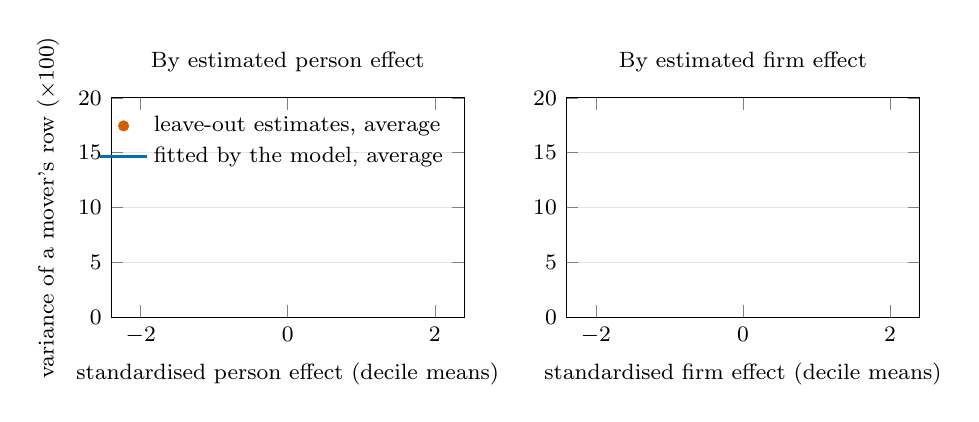
\begin{tikzpicture}
\begin{groupplot}[group style={group size=2 by 1, horizontal sep=1.3cm}, width=0.5\textwidth, height=0.36\textwidth,
  ymin=0, ymax=20, xmin=-2.4, xmax=2.4, ymajorgrids, grid style={gray!20},
  xlabel style={font=\footnotesize}, ylabel style={font=\footnotesize}, ticklabel style={font=\footnotesize},
  title style={font=\footnotesize}, legend style={font=\footnotesize, draw=none, fill=none, legend cell align=left}]
\nextgroupplot[title={By estimated person effect}, xlabel={standardised person effect (decile means)},
  ylabel={variance of a mover's row ($\times100$)}, legend style={at={(0.98,0.97)}, anchor=north east}]
\addlegendimage{only marks, mark=*, mark size=1.8pt, cmove}
\addlegendentry{leave-out estimates, average}
\addlegendimage{no marks, thick, cstay}
\addlegendentry{fitted by the model, average}
\addplot[cmove, only marks, mark=*, mark size=1.8pt, forget plot] coordinates {\figalphalo};
\addplot[cstay, thick, no marks, forget plot] coordinates {\figalphafit};
\nextgroupplot[title={By estimated firm effect}, xlabel={standardised firm effect (decile means)}]
\addplot[cmove, only marks, mark=*, mark size=1.8pt] coordinates {\figpsilo};
\addplot[cstay, thick, no marks] coordinates {\figpsifit};
\end{groupplot}
\end{tikzpicture}
\caption{Movers' rows by decile of the estimated effects: average leave-out estimate $\hat\sigma_i^2$ and average
fitted variance $\st_i^2$. The bin boundaries are deciles of stayers' estimated effects. The plotted observations are movers' rows in the six-year Veneto method study.}
\label{fig:profile}
\end{figure}


\subsection{What changes when the truth is known?}\label{sec:sim}
Holding the six-year network and effects fixed, a method study drew new wages
under ten variance patterns, including flat variances, skewed and fat-tailed errors,
and different wage profiles for movers and stayers. Each scenario had 200 draws, and
each draw ran the estimator as on the data: projected leverages for movers, the two
regressions with estimated effects in the profile, and simulated double sums.
Table~\ref{tab:sim} reports the ratio of the root-mean-square standard error to the
benchmark standard deviation, that is, the square root of the mean variance estimate
over the true variance, together with the coverage of the normal 95\% interval.

\begin{table}[htbp]\centering\small\setlength{\tabcolsep}{4.5pt}
\caption{Simulation on the six-year Veneto design, with the fitted model for movers}
\label{tab:sim}
\begin{tabular}{@{}rl cccc c cccc@{}}
\toprule
 & & \multicolumn{4}{c}{Standard error / benchmark} & & \multicolumn{4}{c}{Coverage of the 95\% interval}\\
\cmidrule(lr){3-6}\cmidrule(l){8-11}
 & Scenario & Worker & Firm & Cov. & Sum & & Worker & Firm & Cov. & Sum\\
\midrule
\tabinput{\srcbase unified/revision/tab_sim_model.tex}
\bottomrule
\end{tabular}
\par\smallskip\begin{minipage}{0.97\linewidth}\footnotesize
A ratio of 1 means that the mean variance estimate equals the true variance. 200 draws
per scenario; the Monte Carlo standard error of a coverage rate is about 0.015. In
scenarios 1 to 7 movers and stayers share one variance profile; in 8 to 10 movers have
their own. Scenarios 3 to 5 depart from the assumed shape of stayers' errors.
\end{minipage}
\end{table}

\emph{The repeat-measurement part is exact.} With the movers' true variances supplied,
the calculation isolates the contribution from repeated wages. In the eight scenarios
without skewness the ratio was 1.00--1.01 for every component, fat tails included.
With skewed stayer errors the ratio for the variance of the sum was 0.97 or 1.03,
depending on the sign of skewness relative to wages. These are the signs predicted by
the calculation in Appendix~\ref{app:proofs}.

\emph{With the fitted model the standard error stays close.} Across the forty
component--scenario cases the ratio lies between 0.96 and 1.10. It is never more than
4\% too small, and coverage is between 93.5\% and 98.0\%. This includes scenario 10,
in which movers follow the decile profile of their own leave-out products in the data
and which is not within the model: its ratios are 1.06 to 1.10.

\emph{Why the ratios lean above one.} Looking only at the ratios would conceal two
opposing contributions. With true effects and true variances as inputs to the fit,
misspecification alone would understate the standard error for the variance of the sum
by 4--8\% in eight scenarios. One source is the cap: where true variances keep rising
beyond three standard deviations, the 1\% of rows beyond the cap can carry a third of
the first term, and raising the cap from three to six standard deviations would move
the predicted ratio in that scenario from 0.95 to 0.99. Using estimated effects and
fitting on noisy wages, together with the other steps of the calculation, moved the
result in the opposite direction, often by more. The comparison cannot attribute the
difference to any one step, and no result predicts its sign in other designs.

\begin{table}[htbp]\centering\small\setlength{\tabcolsep}{4pt}
\caption{Validation with tolerances fixed in advance: ratio and coverage by design}
\label{tab:val}
\begin{tabular}{@{}lc cccc cc@{}}
\toprule
 & & \multicolumn{4}{c}{Standard error / benchmark (range)} & & \\
\cmidrule(lr){3-6}
Design & Scenarios & Worker & Firm & Cov. & Sum & Coverage & Met\\
\midrule
\tabinput{\srcbase note/gen/tab_val.tex}
\bottomrule
\end{tabular}
\par\smallskip\begin{minipage}{0.97\linewidth}\footnotesize
200 fresh draws per scenario. Ranges are over scenarios; coverage is the smallest and
largest value over scenarios and components. \emph{Met}: whether the design met every
registered tolerance. Registered tolerances: for every scenario and component a
ratio between 0.93 and 1.15 and coverage of at least 0.90; for every design an average
coverage of at least 0.94, no failed draw, no nonpositive variance estimate, and
floors binding for at most 2\% of movers' rows in any draw.
\end{minipage}
\end{table}

\emph{The results hold on fresh draws and on two other designs.} The ten scenarios
also informed the choice of model. The estimator was then frozen and run once more
with tolerances written down in advance, on fresh draws of the six-year design, on a
random half of its workers, and on a three-year window (Table~\ref{tab:val}). The
six-year and half-worker runs met every tolerance, and the six-year ratios reproduced
those of Table~\ref{tab:sim} to within 0.007. In the three-year window the
firm-variance standard error was 1.152 and 1.162 times its benchmark in two scenarios,
above the registered limit of 1.15. Across the 88 cases of the three designs the ratio
was below 0.95 in one and above 1.10 in eleven. Shorter panels give less information
about each worker's effect, and there the standard error of firm variance errs on the
conservative side by up to a sixth.

\subsection{What the \texorpdfstring{$q=1$}{q=1} interval adds at a bottleneck}\label{sec:q1sim}
A separate study built synthetic panels with a bottleneck of chosen width: 100 firms
in two groups of 50, 12,000 workers observed for two to six years, and $b$ bridging
workers who move once between the groups. The link has $b=100$, 30 or 10 workers, or
there is no bottleneck. Error variances are flat, follow a wage profile, are steeper
for movers, or are three times as high for the bridging workers alone, a feature the
mover model cannot see. The designs, 1,000 draws per design, and the tolerances were
fixed beforehand. The study tests the $q=1$ construction of
Section~\ref{sec:q1int} applied to every draw, not the automatic choice.

\begin{table}[htbp]\centering\footnotesize\setlength{\tabcolsep}{4.5pt}
\caption{Coverage of 95\% intervals with a bottleneck of $b$ bridging workers}
\label{tab:q1}
\begin{tabular}{@{}l c c c c c c c c@{}}
\toprule
 & & & \multicolumn{4}{c}{Coverage (smallest to largest)} & \multicolumn{2}{c}{Length of $q=1$} \\ \cmidrule(lr){4-7}\cmidrule(l){8-9}
Bottleneck & $\max_iw_{i1}^2$ & $\kappa$ & Normal & $q=1$ & Leave-out & True $\Sigma$ & /normal & /true $\Sigma$ \\
\midrule
None & .157--.167 & 0.05--0.28 & .939--.964 & .941--.970 & .941--.967 & .945--.963 & 1.04 & 1.01 \\
$b=100$ & .010 & 0.30--1.42 & .708--.956 & .951--.986 & .944--.984 & .953--.982 & 1.28 & 1.02 \\
$b=30$ & .031 & 0.95--5.09 & .528--.935 & .973--.993 & .935--.986 & .966--.990 & 1.60 & 1.08 \\
$b=10$ & .090 & 2.74--11 & .487--.937 & .970--1.00 & .795--.911 & .971--.996 & 1.90 & 1.19 \\
\addlinespace
$b=30,10$, skewed errors & .031--.090 & 1.11--9.90 & .743--.923 & .972--.995 & .812--.967 & .977--.993 & 1.60 & 1.08 \\
$b=30,10$, noisy bridge & .031--.090 & 2.77--23 & .629--.727 & .950--.991 & .921--.991 & .982--.996 & 2.25 & 1.00 \\
$b=3$ (stress test) & .256 & 11--35 & .713--.805 & .940--.980 & .710--.833 & .939--.989 & 2.16 & 1.11 \\
\bottomrule
\end{tabular}

\par\smallskip\begin{minipage}{0.97\linewidth}\footnotesize
1,000 draws per design; ranges over designs and over worker variance, firm variance
and the covariance. \emph{Normal}: $\hat\theta\pm1.96\,\widehat{\V}[\hat\theta]^{1/2}$.
\emph{$q=1$}: the interval of Section~\ref{sec:q1int} with \eqref{eq:q1est}.
\emph{Leave-out}: the same with KSS's $V_b^{\rm lo}$ alone. \emph{True $\Sigma$}: the
interval with the true covariance matrix, which no estimate can use. A draw without an
interval counts as not covered. \emph{Length}: mean length of the $q=1$ interval over
that of the normal interval, and over that of the interval with the true matrix.
$\max_iw_{i1}^2$ is the largest squared weight of one row in the leading direction and
$\kappa$ the curvature. Noisy bridge: the bridging workers' errors have three times
the variance.
\end{minipage}
\end{table}

\emph{The $q=1$ interval covers throughout.} All 27,000 draws produced a $q=1$
interval. Across the 75 registered component--design cases it covered between 94.1\%
and 100\%, on average 97.8\%, including with skewed errors and with noisy bridging
workers (Table~\ref{tab:q1}). It is conservative, and most of that is the construction
of KSS and not the estimates: with the true covariance matrix coverage is 94.5\% to
99.6\%.

\emph{The normal interval fails as the bottleneck narrows.} Its coverage falls to
48.7\% with ten bridging workers. The estimate is then far from normal, and the
variance estimate is nonpositive in up to 47.8\% of the draws. Where bridging workers
are noisier than the model can know, the normal standard error is 0.59 to 0.67 times
the true one. For the variance of the sum, which has no dominant direction, the normal
standard error is 1.00 to 1.06 times the true one in every design.

\emph{The larger-of-two rule earns its place.} With ten bridging workers KSS's
leave-out variance of the score alone gives coverage of 79.5--91.1\%, because the
products of a few rows are too noisy. With noisy bridging workers the fitted variance
alone is about a third of the true value and its interval covers 80.3--92.5\%. The
larger of the two covers in both situations.

One registered tolerance was missed. Without a bottleneck the $q=1$ interval was to be
at most 10\% longer than the normal one, and for the covariance in one design it was
12.7\% longer. The interval is not wrong there: it covered 96.9\% against 94.9\% for
the normal one. The result stands as a failure of the tolerance. A stress test with
only three bridging workers lies outside the coverage result
(Appendix~\ref{app:evidence}).

\subsection{Coverage of the interval selected by the command}\label{sec:impl-mc}
The coverage question for a user is whether the interval actually reported
contains the true component. A draw that yields no interval counts as a miss.
The package experiments applied the Stata command to two-block networks of
about 48,000 person-years, ranging from well connected to a single pronounced
bottleneck. They included both deletion modes, normal and skewed errors, and
variance patterns both within and outside the fitted model. Each confirmation
used 20 designs, two deletion modes and 1,000 replications per combination, which
gives 160 cases of a design, a deletion mode and a component.

\begin{table}[htbp]\centering
\caption{Registered confirmations of nominal 95\% intervals through the command}
\label{tab:impl-mc}
\begin{tabular}{@{}lrrrl@{}}
\toprule
Confirmation & Fits & Lowest coverage & Mean coverage & Outcome\\
\midrule
Without controls, first & 40,000 & 0.937 & 0.960 & Failed inventory\\
Without controls, second & 40,000 & 0.930 & 0.959 & Passed\\
With controls & 40,000 & 0.923 & 0.960 & Passed\\
\bottomrule
\end{tabular}
\par\smallskip\begin{minipage}{0.92\linewidth}\footnotesize
Coverage is over replications within a case; lowest and mean are over the 160 cases.
Registered tolerances: coverage of at least 0.92 in every case and 0.94 on average,
an interval for all four components in at least 99\% of the replications of a design
and deletion mode, and, without a bottleneck, a reported interval of median length at
most 1.10 times the normal one with \code{e(V)} posted in at least half of the
samples. In the first run one fit of 40,000 returned point estimates only. The
validation program of the time had no rule for that documented fallback and rejected
its task, so the registered verdict is a failure and stands; counting the fit as a
miss, every tolerance was met, and the coverage figures shown are descriptive. The
no-control confirmations used build \code{fb49e16d} and the controls confirmation
\code{f3938986}. These are pre-release builds; Appendix~\ref{app:evidence} describes
how far the evidence carries to the released package.
\end{minipage}
\end{table}

\emph{The reported interval covers.} In the two passed confirmations none of the
80,000 fits failed or fell back to point estimates. Over their 320 cases the reported
95\% interval covered 96.0\% on average, between 92.3\% and 99.6\% case by case. It
covered at least 95\% in 239 cases and less than 94\% in 16.

\emph{How to read the lowest case.} With 1,000 replications a coverage rate has a
sampling standard error of about 0.007. If every case had exactly 95\% coverage, the
lowest of 160 independent cases would typically be 0.931, and 0.935 if only 40 were
independent, as when the four components of a fit move together. The lowest case
without controls, 0.930, is therefore what nominal coverage looks like. The lowest case
with controls, 0.923, is a real but small shortfall, discussed below.

\emph{The switch is what delivers this.} On the second no-control confirmation, using
normal intervals throughout would have given a lowest coverage of 78.9\% on the same
replications, compared with 93.0\% for the selected interval. The switch costs little
where it is not needed: without a bottleneck the selected interval was at most 1.059
times as long as the normal one, and the command returned a joint covariance in 89\%
of those samples. Selecting the 10\% threshold involved a trade-off. In the development
runs, lowering it to 5\% raised the lowest coverage from 93.7\% to 94.0\%, but more
than doubled the frequency of selecting $q=1$ without a bottleneck, from 4.3\% to
9.8\%.

\emph{Controls.} The controls confirmation used new seeds and four kinds of controls.
Its lowest coverage occurred where the two blocks differed and a control loaded on the
worker effect. The worker- and firm-variance standard errors were 8\% and 7\% below
the spread of the estimates there. Separate development stress tests show why the
distinction between joint and fixed-offset estimation matters. In one case without a
bottleneck, under match deletion and with a control index as large as the effects, the
joint estimate's covariance-component standard error was 12\% too small. With a fixed
offset on the same design, the component standard errors ranged from 0.99 to 1.07 of
the spread. By registered design the controls confirmation excluded this large-index
case, variances that move with a control inside a cell, and a control loaded on the
firm effect when the blocks differ.

\section{Comparison with KSS}\label{sec:kss}\label{kss:sec:empirical}
\subsection{The same point estimator, three sources of variance information}
The split-sample procedure in KSS (2020) allows arbitrary heteroskedasticity.
It predicts the mean of an observation along two disjoint paths in the
mobility network and uses products formed from separate predictions. Where
the network cannot supply the paths or products it needs, it substitutes a
conservative variance contribution. Its published application reports inference
for firm variance. The model-based procedure in the KSS Matlab package instead
smooths raw leave-out products over leverage $P_{ii}$ and the component's
own weight $B_{ii}$. It fits a separate variance model for each of three
components. \fevc{} uses one set of variance inputs for all four components and their
covariance. Agreement between \fevc{} and the KSS Matlab package is agreement between
two model-based procedures, and both can err if the characteristics they pool over
miss variation in a few influential workers' wages. Agreement with the split-sample
procedure is the stronger check, because that procedure uses no variance model.

\subsection{Firm variance on the six Table IV samples}\label{kss:sec:emp-se}
The six samples of KSS Table~IV pair wages in 1999 and 2001 for pooled,
younger and older Veneto workers. Each group supplies a leave-one-out and
a more tightly connected leave-two-out sample. They were rebuilt from the raw data
with KSS's own code, and all \fevc{} runs in this section use observation deletion,
as KSS do, with the 2001 indicator as the only control. On common rows, with KSS's
year-effect treatment and enough projections, \fevc{} reproduces the KSS
firm-variance point estimates within numerical uncertainty. With two
observations per worker, leaving out one wage leaves the worker effect
pinned down by the other. The two leave-out products of a mover then sum
to the first-difference product used by KSS. The default estimates can
differ slightly because \fevc{} jointly estimates the year effect and approximates
leverages by random projections.

\begin{table}[htbp]\centering
\caption{Firm variance on KSS's Table IV samples: standard errors}\label{tab:six}
\small\begin{tabular}{@{}llrrrr@{}}
\toprule
Sample & Connected set & KSS split & KSS Matlab & \fevc{} & \fevc{} interval\\
\midrule
Pooled & Leave-one-out & .0006$^a$ & .00048 & .00049 & Normal\\
       & Leave-two-out & .0006$^a$ & .00053 & .00052 & Normal\\
Younger & Leave-one-out & .00059 & .00049 & .00052 & Normal\\
        & Leave-two-out & .00058 & .00055 & .00059 & $q=1$\\
Older  & Leave-one-out & .00244 & .00196 & .00199 & $q=1$\\
       & Leave-two-out & .00137 & .00110 & .00094 & $q=1$\\
\bottomrule
\end{tabular}
\par\smallskip\begin{minipage}{0.92\linewidth}\footnotesize
Entries are standard errors of the normal form, the square root of the variance
estimate. The final column identifies the interval reported by the \fevc{} default. In
the three $q=1$ rows the default prints the interval and no standard error; the entry
is the normal-form standard error kept in \code{e(inference\_intervals)}. KSS split
uses the Econometrica replication code, and KSS Matlab uses the model-based procedure
in commit \code{8b957ffe}. $^a$Published KSS values (at their printed precision).
The pooled split-sample reruns were stopped after 23 hours before the first
call finished.
\end{minipage}
\end{table}

Four findings stand out in Table~\ref{tab:six}.
\begin{itemize}
\item \emph{The two model-based standard errors agree.} On five of the six samples
they are within about 7\% of each other.
\item \emph{The interval choice lines up with KSS's intervals.} \fevc{} reports the $q=1$ interval
on exactly the three samples where KSS's $q=1$ and normal intervals differ, and the
normal interval on the three where they coincide.
\item \emph{Where the standard errors differ most, the intervals agree.} On the older
leave-two-out sample the standard errors range from .00094 for \fevc{} to .00137 for
KSS's split-sample calculation. Yet the reported $q=1$ intervals are almost identical:
$[.0154,.0218]$ for \fevc{} and $[.0155,.0220]$ for KSS. Those intervals depend on the
joint uncertainty of the leading score and the remainder, which a normal standard
error alone cannot summarise.
\item \emph{The split-sample standard errors are the largest where they are
conservative by construction.} On the leave-one-out samples, 15--22\% of movers lack
an independent second path and receive KSS's conservative substitution.
\end{itemize}
For worker variance and the covariance, for which KSS publish no standard errors,
the only comparison is the KSS Matlab package. The two agree within 6\% on the pooled
samples and within 11\% on the older samples, with no consistent sign. On the younger
samples the \fevc{} standard errors are 12--25\% larger.

\emph{Time.} On these samples \fevc{} took 18--96 seconds for all four components and
their covariance. The KSS Matlab package took roughly ten minutes to ten hours for
three components. The split-sample Table~IV driver took about thirteen minutes on the
older leave-two-out sample for its two calls on firm variance, and the pooled runs
were stopped after 23 hours. These are observed times on comparable cluster
nodes with different speeds, worker counts, leverage calculations and outputs.
They indicate orders of magnitude. The shared variance fit and the trace
calculation in \eqref{eq:sim} explain part of the difference.

\subsection{Against a known truth}\label{kss:sec:synth}
On real data there is no benchmark that determines which standard error is
closer. A simulation on the two older-worker networks, where the methods differ most,
preserves their actual moves and draws new wages from a version of KSS's Monte Carlo
design. Stayers have no wage noise, and each mover has one observation per employer,
so the simulation is a direct test of the fitted mover model. The design makes the
variance depend partly on the mover's weight $B_{ii}$ in the firm-variance estimator.
That characteristic is an input of the KSS Matlab smoother and is not in the model of
\fevc{}, so the design favours the former. The parameters were fitted on each
older-worker sample; KSS fitted theirs on the pooled sample.

\emph{On the leave-one-out network \fevc{} is on target.} Its firm-variance standard
error and that of the KSS Matlab package are within 4\% of the simulated spread, while
the split-sample standard error is 44\% too large and its intervals are 30\% longer.
The \fevc{} standard errors for worker variance and the covariance are 1\% and 4\%
below the spread, and its reported intervals cover about 97\% for all three
components.

\begin{table}[htbp]\centering
\caption{Older leave-two-out network: standard errors and coverage when the truth is known}
\label{tab:known}
\small\setlength{\tabcolsep}{4pt}\begin{tabular}{@{}llrrr@{}}
\toprule
Component & Procedure & Mean SE bias & Normal coverage & Reported coverage\\
\midrule
Firm variance & KSS split-sample & $+10\%$ & 95.5\% & 97.5\%\\
              & KSS Matlab model-based & $-5\%$ & 88.0\% & 76.5\%\\
              & \fevc{} default & $-6\%$ & 92.0\% & 98.9\%\\
\addlinespace
Worker variance & KSS Matlab model-based & $+2\%$ & 93.5\% & 95.5\%\\
                & \fevc{} default & $-14\%$ & 89.0\% & 97.6\%\\
Worker--firm covariance & KSS Matlab model-based & $+1\%$ & 90.0\% & 96.0\%\\
                        & \fevc{} default & $-15\%$ & 88.1\% & 97.5\%\\
\bottomrule
\end{tabular}
\par\smallskip\begin{minipage}{0.92\linewidth}\footnotesize
All simulated mover noise falls on the second year's wage in this design.
Bias compares the mean normal-form standard error with the standard
deviation across 1,000 \fevc{} estimates, net of numerical projection noise.
Normal coverage is that of the normal interval, which the \fevc{} default does not
report here. Reported coverage uses the selected interval, counting missing or invalid
intervals as misses; the KSS procedures use $q=1$ here. KSS procedures used the first 200
draws, so their coverage rates are less precise than those from 1,000.
\end{minipage}
\end{table}

\emph{On the leave-two-out network the reported intervals cover.} One direction
dominates there. For firm variance \fevc{} reported the $q=1$ interval on every draw,
and that interval has the same median length as the split-sample interval,
0.0086, with coverage of 98.9\% against 97.5\% (Table~\ref{tab:known}). The KSS Matlab
procedure produced shorter intervals (median length 0.0076), but 19\% of its $q=1$
intervals failed the study's validity criterion and counted as misses
(Appendix~\ref{app:evidence} gives the scoring convention). For worker variance and
the covariance the \fevc{} intervals covered 97.6\% and 97.5\%, and 96.1\% and 96.6\%
when the simulated noise is split across the two years.

\emph{The normal-form standard errors fall short on this network.} For firm variance
the shortfall is 6\%. For worker variance and the covariance it is 14--15\%, and
16--17\% with split noise, and normal intervals would cover only 88--89\%. As in the
noisy-bridge designs of Section~\ref{sec:q1sim}, the fitted model is wrong on exactly
the rows that carry the component. This is the situation in which the default does not
report a normal interval.

\emph{The shortfall traces to about thirty movers.} A single direction accounts for
95\% of the sampling variance of estimated worker variance and 92\% for the
covariance. The ten movers with the largest weights carry half the weight of that
direction. Their fitted error variances are just 44--48\% of their true values. Most
of the direction's weight is in leverage deciles six through nine, so inspecting only
the highest-leverage observations would miss it. Fitting the same model directly to
the true variances gives nearly the same discrepancy along the direction: the
functional form, not sampling noise, explains the shortfall. The larger-of-two rule of
Section~\ref{sec:q1int} is what protects the reported interval, because KSS's
leave-out variance of the leading score does not depend on the model.

This example gives content to $b(\Delta)$ in \eqref{eq:b}. An error in the
model matters to the extent that it falls on the workers who carry a
particular component. Whether actual wage noise rises on these links is
unknown. The coefficient on the firm-variance weight in the older sample
has the opposite sign from the estimate on KSS's pooled sample, and the
regression used to calibrate noise explains only 0.9\% of the variation
in the raw products. The simulation is therefore best read as a stress test: it shows
what happens when wage noise is tied to the very weights that carry a component, and
that the reported interval holds up even then.


\section*{References}
\addcontentsline{toc}{section}{References}
Andrews, I. and A. Mikusheva (2016). A geometric approach to nonlinear econometric models. \emph{Econometrica}
84(3), 1249--1264.

\noindent Kline, P., R. Saggio and M. S{\o}lvsten (2018). Leave-out estimation of variance components. arXiv:1806.01494v1,
June 2018.

\noindent Kline, P., R. Saggio and M. S{\o}lvsten (2020). Leave-out estimation of variance components.
\emph{Econometrica} 88(5), 1859--1898.

\noindent Kline, P., R. Saggio and M. S{\o}lvsten (2020). Replication package for ``Leave-out estimation of variance
components'' (the Econometrica replication code, folder \code{Replication ECTA}).

\noindent Kline, P., R. Saggio and M. S{\o}lvsten. LeaveOutTwoWay, a Matlab package for leave-out estimation of
variance components (the ``KSS Matlab package''). GitHub, commit \code{8b957ffe}, October 17, 2024.

\smallskip
\noindent\textit{Source note.} The November 16 method document was prepared by
Claude at Johannes Schmieder's request. This editorial revision was prepared
with Codex from that document, its proofs and its recorded results.
\clearpage
\appendix
\linespread{1.02}\selectfont
\section{Formal results for the baseline estimator}\label{sec:results}

\begin{enumerate}[label=\textbf{A\arabic*.},leftmargin=3em]
\item \textbf{Independent errors.} The errors have mean zero and are independent across rows: across the
matches of a mover and across the years of a stayer. This is the assumption under which $\hat\theta$ is
unbiased; nothing is added to it.
\item \textbf{One variance per stayer.} The rows of stayer $g$ share one variance $\sigma_g^2$. Across stayers
the variances are unrestricted.
\item \textbf{Shape of stayers' errors.} They have zero third moment and the kurtosis of the normal
distribution, $\E\varepsilon_i^4=3\sigma_i^4$. (Any other stated kurtosis can be used, with the adjustment of
Appendix~\ref{app:proofs}.) Movers' errors may have any shape.
\item \textbf{Movers follow the model on average.} Let $v_i^*$ be the fitted value of the model for mover row
$i$ when the true variances are used as outcomes in the two steps \eqref{eq:scale} and \eqref{eq:profile}, and
$\Delta_i=v_i^*-\sigma_i^2$ its error. The weighted error $b(\Delta)$ is defined in \eqref{eq:b}. The assumption is
$b(\Delta)/\V[\hat\theta]\to0$ along the sequence of designs.
Corollary~\ref{cor:transfer} specifies the population fit at fixed characteristics.
\item \textbf{No dominant stayer and no dominant direction.} No single stayer carries more than a small share of
$\V[\hat\theta]$, and no single direction (eigenvalue) accounts for more than a small share of it;
Proposition~\ref{prop:conc} makes both precise.
\end{enumerate}

\smallskip\noindent\textbf{Not assumed:} equal variances across workers or firms; that stayers' variances
follow the profile, or any model; normal errors for movers; any independence that $\hat\theta$ does not itself
assume.

\subsection{Mean and concentration of the variance estimator}
The results come in three steps: the estimator is right on average when movers' variances are known; it
settles down in large samples; and fitting the movers' variances adds an error of known form. All three are for
the exact weights \eqref{eq:ustat}. Proofs are in Appendix~\ref{app:proofs}.

\begin{proposition}[Exact mean]\label{prop:mean}
Assume A1 to A3 and give the movers' rows any non-random numbers $\st_i^2=\sigma_i^2+\Delta_i$ in
\eqref{eq:Vhat}. Then, in every sample,
\[
\E\big[\hat\V[\hat\theta]\big]=\V[\hat\theta]+b(\Delta),
\]
with $b(\Delta)$ as in \eqref{eq:b}. In particular $\hat\V[\hat\theta]$ is unbiased when movers' rows receive
their true variances.
\end{proposition}

The stayers' part of the estimator is therefore exact in finite samples, whatever the stayers' variances are.
An error in the movers' variances enters only through $b(\Delta)$. Its first part weights the errors by
$m_i^2$, so errors that average out against $m_i^2$ do no harm there; its second part is quadratic in the
errors. Both parts count.

\paragraph{When A2 or A3 fails.} The appendix gives the mean of the estimator in three cases. They concern
$\hat\sigma^2_\alpha$ and $\hat\sigma^2_{\alpha+\psi}$ only, because $c_g=0$ for the other two components.
\begin{itemize}
\item \emph{Unequal variances within a stayer.} Because $m_i$ is the same in every year of a stayer, the first
term of \eqref{eq:V} involves a stayer's variances only through their average, and $q_g$ is unbiased for that
average. The terms within the stayer are affected: with normal errors the estimator is too large on average by
$6\sum_gc_g^2\,s_g^2\,(T_g-1)^2(T_g+4)/(T_g(T_g+1))$, where $s_g^2$ is the sample variance of the stayer's $T_g$
variances.
\item \emph{Another kurtosis.} If stayers' errors have kurtosis $\kappa$, its mean shifts by
$2(\kappa-3)\sum_g\sigma_g^4\,c_g^2\,(T_g-1)^2(T_g+4)/(T_g(T_g+1))$: fat tails make the variance estimate too
large.
\item \emph{Skewness.} If stayers' errors have third moments $\mu_{3g}$, its mean shifts by
$8\sum_g(T_g-1)\,c_g\,m_g\,\mu_{3g}$, where $m_g$ is the common value of $m_i$ on the stayer's rows. The shift is
positive when $m_g$ and $\mu_{3g}$ tend to have the same sign, for example when stayers with high person
effects have right-skewed errors and stayers with low person effects left-skewed ones.
\end{itemize}
These terms are not bounded by the adjustment in \eqref{eq:Vhat}: for a stayer with two years the adjustment
is zero and the first two are not. Nor do they vanish in large samples. In a panel that consists of two-year
stayers alone, with equal person effects and equal variances, a kurtosis of $\kappa$ shifts the mean of the variance estimate for
$\hat\sigma^2_\alpha$ by the fraction $(\kappa-3)(G-1)/(2G-1)$ of the variance when there are $G$ stayers,
which tends to $(\kappa-3)/2$. How much
they matter depends on the share of the variance that comes from the pairs of rows within stayers, which is
small when movers' rows carry most of the variance, as in the Veneto panel of Section~\ref{sec:evidence}. The fat-tailed and skewed simulations there violate A3.

\begin{proposition}[Convergence]\label{prop:conc}
Under the assumptions of Proposition~\ref{prop:mean}, suppose $\E\varepsilon_i^8\le\bar c\,\sigma_i^8$ on
stayers' rows, $\E\varepsilon_i^4\le\bar\kappa\,\sigma_i^4$ on movers' rows, and
$|\st_i^2|\le\bth\,\sigma_i^2$ on movers' rows with $\bth\ge1$. Let
\[
\phi_g=\frac{1}{\V[\hat\theta]}\sum_{i\in g}\sigma_i^2\Big(4m_i^2+2\sum_\ell C_{i\ell}^2\sigma_\ell^2\Big)
\]
be the share of the variance \eqref{eq:V} carried by the rows of stayer $g$, and let $\lambda_{\max}$ be the
largest absolute eigenvalue of the matrix with entries $\sigma_iC_{i\ell}\sigma_\ell$. Then
\[
\E\bigg[\Big(\frac{\hat\V[\hat\theta]-\V[\hat\theta]-b(\Delta)}{\V[\hat\theta]}\Big)^{2}\bigg]\;\le\;
c'\,\bth^2\Big(\max_g\phi_g+\frac{\lambda_{\max}^2}{\V[\hat\theta]}\Big),
\]
where $c'$ depends only on $\bar c$ and $\bar\kappa$.
\end{proposition}

So with true variances for movers the ratio $\hat\V[\hat\theta]/\V[\hat\theta]$ converges to one along any
sequence of designs in which the moment bounds hold and (a) no single stayer carries more than a vanishing
share of the variance and (b) $\lambda_{\max}^2/\V[\hat\theta]\to0$. The two design conditions (a) and (b) are
implied by the design conditions of KSS's Theorem~2, under which $\hat\theta$ is asymptotically normal, provided
the number of years per stayer is bounded (Lemma~\ref{lem:kss}). Condition (b) can fail when there are few
firms, or when groups of firms are linked by few movers, which KSS call weak identification; the propositions
then give no guarantee. The bounds concern exact weights and fixed mover inputs.

\begin{proposition}[Fitted variances for movers]\label{prop:fitted}
Assume A1 to A3, the moment bounds of Proposition~\ref{prop:conc}, and Assumption~1 of KSS (uniformly bounded
fourth moments, variances bounded away from zero, leverages bounded away from one, bounded $x_i'\beta$). Let
the movers' rows receive fitted values $\st_i^2$ that may depend on the data, and suppose there are a statistic
$\hat\eta$ of fixed dimension, a non-random $\eta^*$, non-random functions $\psi_i$ and constants
$c_\eta,L,r,\bar\psi$ such that $\st_i^2=\psi_i(\hat\eta)$ for all $i\in\cR$ with probability tending to one,
and
\[
\E\|\hat\eta-\eta^*\|^2\le\frac{c_\eta}{n_0},\qquad
|\psi_i(\eta)-\psi_i(\eta^*)|\le L\,\|\eta-\eta^*\|\ \text{ whenever }\|\eta-\eta^*\|\le r,\qquad
|\psi_i(\eta^*)|\le\bar\psi ,
\]
for all $i\in\cR$. Put $\Delta_i=\psi_i(\eta^*)-\sigma_i^2$. Then, along a sequence of designs with
$n_0\to\infty$ and the constants fixed,
\[
\frac{\hat\V[\hat\theta]}{\V[\hat\theta]}=1+\frac{b(\Delta)}{\V[\hat\theta]}+O_p\bigg(n_0^{-1/2}+
\Big(\max_g\phi_g+\frac{\lambda_{\max}^2}{\V[\hat\theta]}\Big)^{1/2}\bigg).
\]
\end{proposition}

The fitted values may depend on the same data as $\hat m$ in any way; the proof does not use independence
between them.

\begin{corollary}[The model for movers]\label{cor:transfer}
Assume A1 to A3, the moment bounds of Proposition~\ref{prop:conc} and Assumption~1 of KSS. Suppose the
characteristics are non-random and bounded: $z_i$ in \eqref{eq:scale}, and $b_i$ in place of
$b(\tilde\alpha_i,\tilde\psi_i)$ in \eqref{eq:profile}. Let $c_z^*$ and $d^*$ be the results of the two steps when
the true variances $\sigma_i^2$ are used as outcomes, and
\[
v_i^*=s_i^*\,b_i'd^*,\qquad s_i^*=z_i'c_z^* .
\]
Suppose that the smallest eigenvalues of $n_{\cR}^{-1}\sum_{i\in\cR}z_iz_i'$ and of
$n_{\cR}^{-1}\sum_{i\in\cR}s_i^{*2}\,b_ib_i'$ are bounded away from zero, where $n_{\cR}$ is the number of movers'
rows; and that, with probability tending to one, $s_i^*$ and $v_i^*$ exceed their floors by a uniform margin.
Then Proposition~\ref{prop:fitted} applies with $n_0=n_{\cR}$ and
\[
\Delta_i=v_i^*-\sigma_i^2 .
\]
If $\sigma_i^2=s_i^*\,b_i'd$ for all $i\in\cR$ and some $d$, then $\Delta=0$, and
$\hat\V[\hat\theta]/\V[\hat\theta]\to1$ in probability as $n_{\cR}\to\infty$ under A5. This is the case, for
instance, when movers' variances are $\sigma_i^2=(z_i'c)(b_i'd)$ and
$\sum_{i\in\cR}z_i\,(z_i'c)\,(b_i'd-\bar\pi)=0$ for some constant $\bar\pi\neq0$, as when the profile $b_i'd$ has
the same mean at every value of $z_i$.
\end{corollary}


The corollary treats the features of the profile as fixed, with floors asymptotically inactive.
Estimated effects in a short panel can retain estimation error as the panel grows and can share
errors with the leave-out products. The corollary does not establish consistency for that case.
Under the conditions of KSS's Theorem~2, a consistent variance estimate gives an
asymptotically valid normal interval.
\subsection{Simulation of the quadratic term}
\begin{proposition}[Simulated double sum]\label{prop:sim}
Let $\hat\V_{D_s}$ be \eqref{eq:Vhat} with the double sum computed by \eqref{eq:sim}. Under the assumptions of
Proposition~\ref{prop:conc}, with $0\le\st_i^2\le\bth\sigma_i^2$ on movers' rows,
$\E[\hat\V_{D_s}\mid\text{data}]=\hat\V[\hat\theta]$ and
\[
\frac{\E\big[(\hat\V_{D_s}-\hat\V[\hat\theta])^2\big]}{\V[\hat\theta]^2}\;\le\;\frac{c''\,\bth^4}{D_s}\cdot\frac{\lambda_{\max}^2}{\V[\hat\theta]} ,
\]
where $c''$ depends only on $\bar c$.
\end{proposition}
Here $D_s$ is the number of independent draws in \eqref{eq:sim}. For fitted variances the conditional mean
identity still holds. Given the data, the variance of $\hat\V_{D_s}$ is $8\tr(\tilde K^4)/D_s$ with
$\tilde K_{i\ell}=\st_i C_{i\ell}\st_\ell$.
\subsection{Inference with one dominant direction}
\begin{proposition}[The covariance matrix for $q=1$]\label{prop:q1}
Assume A1 to A3, the moment bounds of Proposition~\ref{prop:conc} and Assumption~1 of KSS, suppose
$\Sigma_{\rm rr}>0$, and give the movers' rows non-random numbers $\st_i^2=\sigma_i^2+\Delta_i$ with
$|\st_i^2|\le\bth\,\sigma_i^2$ for a constant $\bth\ge1$. Let
$\phi_g^{\rm r}$ and $\lambda_{\max}^{\rm r}$ be the quantities of Proposition~\ref{prop:conc} for the remainder,
that is, with $C^{\rm r}$, $m^{\rm r}$ and $\Sigma_{\rm rr}$ in place of $C$, $m$ and $\V[\hat\theta]$, and let
$\epsilon_{\rm r}=\max_g\phi_g^{\rm r}+(\lambda_{\max}^{\rm r})^2/\Sigma_{\rm rr}$. Write
$\hat\Sigma_{bb}^{\rm lo}=\sum_iw_{i1}^2\hat\sigma_i^2$ for the leave-out number in \eqref{eq:q1est},
$d_{\rm r}(\Delta)=2\sum_{i\in\cR}w_{i1}m_i^{\rm r}\Delta_i$, and $b_{\rm r}(\Delta)$ for \eqref{eq:b} formed with
$C^{\rm r}$ and $m^{\rm r}$. Then, in every sample,
\[
\E\hat\Sigma_{bb}^{\rm lo}=\Sigma_{bb},\qquad \E\hat\Sigma_{b{\rm r}}=\Sigma_{b{\rm r}}+d_{\rm r}(\Delta),\qquad
\E\hat\Sigma_{\rm rr}=\Sigma_{\rm rr}+b_{\rm r}(\Delta),
\]
and
\begin{align*}
\E\Big[\Big(\frac{\hat\Sigma_{bb}^{\rm lo}}{\Sigma_{bb}}-1\Big)^2\Big]&\le c_b\,\max_iw_{i1}^2,\\
\E\Big[\frac{\big(\hat\Sigma_{b{\rm r}}-\Sigma_{b{\rm r}}-d_{\rm r}(\Delta)\big)^2}{\Sigma_{bb}\,\Sigma_{\rm rr}}\Big]&\le c_{b{\rm r}}\,\bth^2\,\epsilon_{\rm r},\qquad
\E\Big[\Big(\frac{\hat\Sigma_{\rm rr}-\Sigma_{\rm rr}-b_{\rm r}(\Delta)}{\Sigma_{\rm rr}}\Big)^2\Big]\le c'\,\bth^2\,\epsilon_{\rm r},
\end{align*}
where $c_b$, $c_{b{\rm r}}$ and $c'$ depend only on the constants of the assumptions. Consequently, along a
sequence of designs in which $\max_iw_{i1}^2\to0$, $\epsilon_{\rm r}\to0$, $b_{\rm r}(\Delta)/\Sigma_{\rm rr}\to0$,
$d_{\rm r}(\Delta)/(\Sigma_{bb}\Sigma_{\rm rr})^{1/2}\to0$ and $|\rho|$ stays below a number less than one, the matrix
$\hat\Sigma^{\rm lo}$ with entries $\hat\Sigma_{bb}^{\rm lo}$, $\hat\Sigma_{b{\rm r}}$, $\hat\Sigma_{\rm rr}$ satisfies
$\Sigma^{-1/2}\hat\Sigma^{\rm lo}\Sigma^{-1/2}\to I$ in probability. The same holds when the movers' rows receive
the fitted values of Corollary~\ref{cor:transfer}, with $\Delta_i=v_i^*-\sigma_i^2$ and $n_{\cR}\to\infty$.
\end{proposition}

The proposition is about $\hat\Sigma^{\rm lo}$, the matrix with KSS's first entry. The matrix with the rule
\eqref{eq:q1est} need not be consistent: where the fitted variances overstate $\Sigma_{bb}$ its first entry
stays too large. What the rule keeps is coverage. Let $\hat\rho_{\rm lo}$ be the correlation computed from
$\hat\Sigma^{\rm lo}$.

\begin{corollary}[Coverage]\label{cor:q1}
\textup{(a)} In any sample in which $\hat\Sigma^{\rm lo}$ is positive definite and $\hat\rho_{\rm lo}^2\le2/3$, the
interval of Section~\ref{sec:q1int} formed with \eqref{eq:q1est} contains the interval formed with
$\hat\Sigma^{\rm lo}$.
\textup{(b)} Suppose the conditions of the last part of Proposition~\ref{prop:q1} hold, with $|\rho|$ at most a
constant strictly below $(2/3)^{1/2}$, together with the hypotheses of KSS's Theorem~3 for $q=1$: their
Assumptions~1 and~2, $\max_iw_{i1}^2\to0$, and
$\Sigma_{\rm rr}^{-1}\max_i\big((\tilde x_{i1}'\beta)^2+(\check x_{i1}'\beta)^2\big)\to0$. Then the interval formed
with \eqref{eq:q1est} covers $\theta$ with probability of at least $1-\alpha$ in the limit.
\end{corollary}

Part (a) is algebra (Appendix~\ref{app:proofs}); the bound $2/3$ is on the squared correlation before the first entry is
raised, and without it a larger first entry can lower the critical value and move an end point inwards. Part (b)
combines three things: KSS's Theorem~3, under which $\hat b_1$ and $\hat\theta_{\rm r}$ are jointly asymptotically
normal; their Lemma~7, under which the interval with a consistent matrix then covers with probability of at
least $1-\alpha$ in the limit; and part (a), which holds with probability tending to one. The condition on
$\tilde x_{i1}$ and $\check x_{i1}$ says that no single row dominates the linear part of the remainder; it is
KSS's and is not implied by the conditions of the proposition. If the fitted variances overstate $\Sigma_{bb}$ in
large samples, the interval is longer than necessary but its coverage bound stands. The conditions of the
proposition, in words:
\begin{itemize}
\item \emph{No single row dominates $\hat b_1$}: $\max_iw_{i1}^2\to0$. This is the Lindeberg condition of KSS's
Theorem~3. KSS read $1/\max_iw_{i1}^2$ as an effective number of observations behind $\hat b_1$.
\item \emph{The remainder has no dominant stayer and no dominant direction}: $\epsilon_{\rm r}\to0$. When the
years per stayer are bounded, a sufficient condition is the remainder's analogue of KSS's conditions, with the
second eigenvalue set against the remaining ones, $\lambda_2^2/\sum_{\ell\ge2}\lambda_\ell^2\to0$
(Appendix~\ref{app:proofs}). This is stronger than KSS's Assumption~2, which sets $\lambda_2^2$ against the sum
over all eigenvalues.
\item \emph{The model's errors average out for the remainder}, in its variance and in its covariance with
$\hat b_1$: $b_{\rm r}(\Delta)/\Sigma_{\rm rr}\to0$ and $d_{\rm r}(\Delta)/(\Sigma_{bb}\Sigma_{\rm rr})^{1/2}\to0$. This is
A4 for the remainder. Both are zero when movers' variances follow the model.
\item \emph{$\hat b_1$ and the remainder are not collinear.} With equal variances $\rho=0$.
\end{itemize}
No independence beyond A1 is used, and the stayers' part is again exact in the mean: only the third condition
involves the model. The zero third moments of A3 are needed for the mean of $\hat\Sigma_{b{\rm r}}$; with
skewed stayers' errors it shifts by a term given in the appendix. As in Section~\ref{sec:results}, the
proposition evaluates the profile at fixed characteristics; the estimator evaluates it at estimated effects.

{\small\section{Proofs}\label{app:proofs}

\subsection{Setting and notation}

The proofs use the following, more general, statement of the setting. Rows $i=1,\dots,n$ have outcomes
$y_i=\mu_i+\varepsilon_i$ with $\mu_i=x_i'\beta$; the regressors and $\beta$ are non-random. The estimator is
$\hat\theta=\sum_i\sum_\ell C_{i\ell}y_iy_\ell$, with $m=C\mu$, $\hat m=Cy$ and $V=\V[\hat\theta]$. $U$ denotes the
set of rows of a stayer, $\mathcal{U}$ the collection of these sets (one per stayer), $|U|\ge2$ the number of rows
of $U$ and $d_U=|U|-1$; $R$ is the set of movers' rows ($\cR$ in the text).

\begin{enumerate}[label=\textbf{(S\arabic*)},leftmargin=3.3em,itemsep=3pt]
\item \textbf{Independent errors.} $\varepsilon_1,\dots,\varepsilon_n$ are independent, with $\E\varepsilon_i=0$
and $0<\sigma_i^2=\E\varepsilon_i^2<\infty$.
\item \textbf{Exact weights.} $C$ is a non-random symmetric matrix with $C_{ii}=0$ for all $i$, and for every
$U\in\mathcal{U}$ there is a number $c_U$ with $C_{i\ell}=c_U$ for all $i\ne\ell$ in $U$. (Lemma~\ref{lem:stayer}:
the weights \eqref{eq:ustat} have this property.)
\item \textbf{Stayers.} The sets $U\in\mathcal{U}$ are pairwise disjoint and are determined by the regressors.
Within a set the means are equal, $\mu_i=\mu_U$, and so are the variances, $\sigma_i^2=\tau_U$. With
$\bar y_U$ the mean of the outcomes of $U$,
\[
q_U=\frac{1}{d_U}\sum_{i\in U}(y_i-\bar y_U)^2,
\]
and every row of $U$ receives $\st_i^2=q_U$. ($q_U$ is $q_g$ of \eqref{eq:q} and $\tau_U$ is $\sigma_g^2$.)
\item \textbf{Stayers' errors.} For every row $i$ of a set, $\E\varepsilon_i^3=0$,
$\E\varepsilon_i^4=\kappa\,\sigma_i^4$ and $\E\varepsilon_i^8\le\bar c\,\sigma_i^8$. The text takes $\kappa=3$;
the proofs allow any $\kappa\ge1$.
\item \textbf{Movers' rows.} For $i\in R$, $\E\varepsilon_i^4\le\bar\kappa\,\sigma_i^4$ for a constant
$\bar\kappa\ge\kappa$. These rows receive $\st_i^2=\sigma_i^2+\Delta_i$ with non-random numbers $\Delta_i$.
\item $V>0$.
\end{enumerate}
S1 to S3 are A1 and A2 of the text, S4 is A3 with the moment bound of Proposition~\ref{prop:conc}, and nothing
is asked of the third moments or the kurtosis of movers' errors.

\paragraph{The estimator.} For a stated kurtosis $\kappa$ let
\begin{equation}\label{eq:nuh}
\nu_U=\frac{2}{|U|-1}+\frac{\kappa-3}{|U|},\qquad
\chi_U=c_U^2\big[4\,(2-|U|)+2\,(\kappa-3)\,(|U|-1)\big],\qquad \bnu=2+|\kappa-3| ,
\end{equation}
and
\begin{equation}\label{eq:VhatA}
\hat V=4\sum_i\hat m_i^{\,2}\,\st_i^2-2\sum_i\sum_\ell C_{i\ell}^2\,\st_i^2\,\st_\ell^2
-\sum_{U\in\mathcal{U}}\chi_U\,\frac{q_U^2}{1+\nu_U}.
\end{equation}
For $\kappa=3$, $\chi_U/(1+\nu_U)=-4c_U^2(|U|-2)(|U|-1)/(|U|+1)$, and \eqref{eq:VhatA} is
$\hat\V[\hat\theta]$ of \eqref{eq:Vhat}. $b(\Delta)$ is defined in \eqref{eq:b}.

\paragraph{Standardised notation.} Let $u_i=\varepsilon_i/\sigma_i$, $a_i=\sigma_im_i$ and
$K_{i\ell}=\sigma_iC_{i\ell}\sigma_\ell$, so that $K$ is symmetric with zero diagonal, and let $w=a+Ku$, so that
$\sigma_i\hat m_i=w_i$. For index sets $I,J$, $K_{IJ}$ is the block of $K$ with rows in $I$ and columns in $J$,
$K_{I\cdot}$ the rows in $I$, and $u_I$, $a_I$, $w_I$ the subvectors. $\|\cdot\|$ is the Euclidean norm of a vector
and the Frobenius norm of a matrix; $\|\cdot\|_\op$ is the operator norm. We use $\|XY\|\le\|X\|_\op\|Y\|$,
$\|X\|_\op\le\|X\|$ and $|\tr(XY)|\le\|X\|\,\|Y\|$ freely.

For $U\in\mathcal{U}$ let $\Pi_U=I-\mathbf{1}\mathbf{1}'/|U|$, the projection that removes the mean of the set, and
$\bar Q_U=\Pi_U/d_U$. Since the means are equal within $U$ and $\varepsilon_i=\sqrt{\tau_U}\,u_i$ on $U$,
\begin{equation}\label{eq:xi}
\xi_U:=\frac{q_U}{\tau_U}-1=u_U'\,\bar Q_U\,u_U-1,\qquad \st_i^2=\sigma_i^2\,(1+\xi_U)\ \ (i\in U).
\end{equation}
$\xi_U$ depends on $u_U$ only, so the $\xi_U$ are independent across sets, and $\xi_U$ is independent of the errors
outside $U$. Put $\xi_i=\xi_U$ for $i\in U$ and $\xi_i=0$ for $i\in R$, and let
\begin{equation}\label{eq:G}
G_U=2\,\bar Q_U+(\kappa-3)\diag\big(\bar Q_U\big)=2\,\bar Q_U+\frac{\kappa-3}{|U|}\,I .
\end{equation}
Note that $\tr(\bar Q_U^2)=1/d_U$ and that the diagonal entries of $\bar Q_U$ equal $1/|U|$, so that
$\nu_U=2\tr(\bar Q_U^2)+(\kappa-3)\sum_{j\in U}\bar Q_{U,jj}^{\,2}$.

For the movers' rows let $\vartheta_i=1+\Delta_i/\sigma_i^2$ ($i\in R$), $\vartheta_i=1$ for rows in sets,
$\Theta=\diag(\vartheta_i)$ and $\bth=\max(1,\max_{i\in R}|\vartheta_i|)$. Then
$\st_i^2=\sigma_i^2\,\vartheta_i\,(1+\xi_i)$ for every row, and \eqref{eq:VhatA} reads
\begin{equation}\label{eq:pieces}
\begin{aligned}
\hat V&=P_1+P_2+P_3+P_4, &
P_1&=4\,w'\Theta w, \qquad P_2=4\sum_{U\in\mathcal{U}}\xi_U\,\|w_U\|^2,\\
P_3&=-2\sum_i\sum_\ell K_{i\ell}^2\,\vartheta_i\vartheta_\ell\,(1+\xi_i)(1+\xi_\ell), &
P_4&=-\sum_{U\in\mathcal{U}}\tau_U^2\,\chi_U\,\frac{(1+\xi_U)^2}{1+\nu_U}.
\end{aligned}
\end{equation}
(For the first term, $\hat m_i^{\,2}\st_i^2=w_i^2\vartheta_i(1+\xi_i)$, and $\vartheta_i=1$ where $\xi_i\ne0$.)
By Lemma~\ref{lem:forms} below, $V=4\|a\|^2+2\|K\|^2$, which is \eqref{eq:V}. Let $k_{UU'}=\|K_{UU'}\|^2$,
$k_U=\|K_{U\cdot}\|^2=\sum_{i\in U}\sum_\ell K_{i\ell}^2$, $\rho_U=\|a_U\|^2+k_U$, and let
$\lambda=\lambda_{\max}=\|K\|_\op$. The share of Proposition~\ref{prop:conc} is $\phi_U=(4\|a_U\|^2+2k_U)/V$. Since
the sets are disjoint,
\begin{equation}\label{eq:facts}
2\rho_U\le\phi_UV,\qquad \sum_{U}\rho_U\le\|a\|^2+\|K\|^2\le\tfrac12V,\qquad
\sum_{U'\in\mathcal{U}}k_{UU'}\le k_U,\qquad k_{UU}\le k_U\le\rho_U .
\end{equation}
All results are bounds for one design with explicit constants; along a sequence of designs the constants of
the assumptions are the same for every design.

\subsection{Lemmas}

\begin{lemma}[A stayer's weights]\label{lem:stayer}
\textup{(a)} For the weights \eqref{eq:ustat} and two rows $i\ne\ell$ of stayer $g$: $P_{i\ell}=1/T_g$,
$B_{i\ell}=A_{gg}/T_g^2$ and $C_{i\ell}=A_{gg}/(T_g(T_g-1))$; moreover $m_i=m_\ell$.
\textup{(b)} Under S2, $K_{UU}=\tau_Uc_U(\mathbf{1}\mathbf{1}'-I)$, and with $e_U:=\tr(K_{UU}^2G_U)$,
\[
4\,e_U-2\,\nu_U\,k_{UU}=\tau_U^2\,\chi_U,\qquad \tau_U^2\,|\chi_U|\le\bnu\,k_{UU} .
\]
\end{lemma}

\begin{proof}
(a) The rows of stayer $g$ have the same regressor vector $x_i=x_g$, and no other row involves the person effect
of $g$. Let $\epsilon_g$ be the unit vector of that effect. Then
$S_{xx}\epsilon_g=\sum_jx_j(x_j'\epsilon_g)=T_gx_g$, so $S_{xx}^{-1}x_i=\epsilon_g/T_g$. Hence
$P_{i\ell}=x_i'\epsilon_g/T_g=1/T_g$ and $B_{i\ell}=\epsilon_g'A\epsilon_g/T_g^2=A_{gg}/T_g^2$, also for $i=\ell$.
With $M_{i\ell}=-1/T_g$ and $M_{ii}=1-1/T_g$, \eqref{eq:ustat} gives
$C_{i\ell}=\frac{A_{gg}}{T_g^2}\big(1+\frac{1}{T_g-1}\big)=\frac{A_{gg}}{T_g(T_g-1)}$. Finally
$m_i-m_\ell=\sum_{j\ne i}C_{ij}\mu_j-\sum_{j\ne\ell}C_{\ell j}\mu_j=C_{i\ell}(\mu_\ell-\mu_i)=0$, because the rows
$i$ and $\ell$ of $C$ agree outside the columns $i$ and $\ell$ and $\mu_i=\mu_\ell$.
(b) Write $t=|U|$ and $J=\mathbf{1}\mathbf{1}'$. The first claim is S2 with $\sigma_i^2=\tau_U$ on $U$. Then
$K_{UU}^2=\tau_U^2c_U^2\big((t-2)J+I\big)$, so $k_{UU}=\tr K_{UU}^2=\tau_U^2c_U^2\,t(t-1)$, and, since $J\Pi_U=0$,
$\tr(K_{UU}^2\bar Q_U)=\tau_U^2c_U^2\tr(\Pi_U)/d_U=\tau_U^2c_U^2$. By \eqref{eq:G} and \eqref{eq:nuh},
\[
4e_U-2\nu_Uk_{UU}=\tau_U^2c_U^2\Big[8+4(\kappa-3)(t-1)-4t-2(\kappa-3)(t-1)\Big]=\tau_U^2\chi_U .
\]
For the bound, $|2-t|\le t-1$ gives $|\chi_U|\le c_U^2(t-1)(4+2|\kappa-3|)=2\bnu\,c_U^2(t-1)$, and
$c_U^2(t-1)\tau_U^2=k_{UU}/t\le k_{UU}/2$.
\end{proof}

In Lemma~\ref{lem:forms}, $u_1,\dots,u_N$ are independent with $\E u_j=0$, $\E u_j^2=1$ and
$\kappa_j:=\E u_j^4\le\bar\kappa$. Nothing is assumed about third moments. Put
$c_4=\max(3,\bar\kappa)$.

\begin{lemma}[Linear and quadratic forms]\label{lem:forms}
Let $b\in\mathbb{R}^N$, $M$ a symmetric $N\times N$ matrix, $a\in\mathbb{R}^t$ and $F$ a $t\times N$
matrix, all non-random.
\begin{enumerate}[label=\textup{(\alph*)}]
\item $\E(b'u)^2=\|b\|^2$ and $\E(b'u)^4=3\|b\|^4+\sum_j(\kappa_j-3)\,b_j^4\le c_4\|b\|^4$.
\item $\E[u'Mu]=\tr M$ and $\Var(u'Mu)=2\|M\|^2+\sum_j(\kappa_j-3)M_{jj}^2\le\max(2,\bar\kappa-1)\,\|M\|^2$.
If $M$ has zero diagonal, then $\Var(u'Mu)=2\|M\|^2$ and $\E[(b'u)(u'Mu)]=0$, and these two
statements need second moments only.
\item $\E\|a+Fu\|^4\le4c_4\big(\|a\|^2+\|F\|^2\big)^2$.
\item If $M$ has zero diagonal, $\E(u'Mu)^4\le(256+24\bar\kappa)\,c_4\,\|M\|^4$.
\item If in addition $\E u_j^8\le\bar c$ for all $j$, then $\E(u'Mu-\tr M)^4\le c_Q\,\|M\|^4$ with
$c_Q=6720\,\bar c$. If $M$ is also positive semidefinite, $\E(u'Mu)^4\le8\,(c_Q+1)\,(\tr M)^4$.
\end{enumerate}
\end{lemma}

\begin{proof}
A product of errors has expectation zero whenever some error occurs in it exactly once (independence
and mean zero). Call this the \emph{single-index rule}.

(a) The second moment is immediate. In
$\E(b'u)^4=\sum b_{j_1}b_{j_2}b_{j_3}b_{j_4}\E[u_{j_1}u_{j_2}u_{j_3}u_{j_4}]$ the single-index rule
leaves the terms with four equal indices, $\sum_jb_j^4\kappa_j$, and those with two distinct indices
each occurring twice, $3\sum_{j\ne\ell}b_j^2b_\ell^2=3\|b\|^4-3\sum_jb_j^4$. For the bound,
$\sum_jb_j^4\le\|b\|^4$, so the fourth moment is at most $3\|b\|^4$ if $\bar\kappa\le3$ and at most
$\bar\kappa\|b\|^4$ otherwise.

(b) Write $u'Mu-\tr M=D+O$ with $D=\sum_jM_{jj}(u_j^2-1)$ and $O=2\sum_{j<\ell}M_{j\ell}u_ju_\ell$.
The summands of $D$ are independent with mean zero and variances $M_{jj}^2(\kappa_j-1)$. Each summand
of $O$ has mean zero and variance $4M_{j\ell}^2$, and by the single-index rule it is uncorrelated
with every other summand of $O$, with every summand of $D$ and with $b'u$. Hence
$\Var(u'Mu)=\sum_jM_{jj}^2(\kappa_j-1)+2\sum_{j\ne\ell}M_{j\ell}^2$, which is the formula. It is
at most $2\|M\|^2$ if $\bar\kappa\le3$ and at most $2\|M\|^2+(\bar\kappa-3)\sum_jM_{jj}^2
\le(\bar\kappa-1)\|M\|^2$ otherwise. With zero diagonal, $D=0$ and no fourth moment enters.

(c) Let $g=a+Fu$ with coordinates $g_i=a_i+f_i'u$, $f_i'$ the $i$th row of $F$. By Minkowski's
inequality in $L^4$ and (a), $(\E g_i^4)^{1/4}\le|a_i|+c_4^{1/4}\|f_i\|$, so
$(\E g_i^4)^{1/2}\le2a_i^2+2c_4^{1/2}\|f_i\|^2\le2c_4^{1/2}(a_i^2+\|f_i\|^2)$. By Minkowski's inequality in
$L^2$, $(\E\|g\|^4)^{1/2}=\big(\E(\sum_ig_i^2)^2\big)^{1/2}\le\sum_i(\E g_i^4)^{1/2}
\le2c_4^{1/2}(\|a\|^2+\|F\|^2)$.

(d) Let $L_k=\sum_{i<k}M_{ik}u_i$ (with $L_1=0$), $\gamma_k=2u_kL_k$ and $S_k=\sum_{j\le k}\gamma_j$, so that
$u'Mu=S_N$. $L_k$ is a function of $u_1,\dots,u_{k-1}$, so $\E[\gamma_k\mid u_1,\dots,u_{k-1}]=0$:
$(S_k)$ is a martingale. By (a), $\E L_k^4\le c_4\ell_k^2$ with $\ell_k=\sum_{i<k}M_{ik}^2$; hence
$L_k$, $\gamma_k$ and $S_k$ have finite fourth moments. Expanding $(S_{k-1}+\gamma_k)^4$,
\[
\E S_k^4=\E S_{k-1}^4+4\,\E[S_{k-1}^3\gamma_k]+6\,\E[S_{k-1}^2\gamma_k^2]+4\,\E[S_{k-1}\gamma_k^3]+\E\gamma_k^4 .
\]
The second term is $8\,\E[S_{k-1}^3L_k]\,\E[u_k]=0$. For the fourth,
$4|S_{k-1}\gamma_k^3|\le2S_{k-1}^2\gamma_k^2+2\gamma_k^4$. So
$\E S_k^4\le\E S_{k-1}^4+8\,\E[S_{k-1}^2\gamma_k^2]+3\,\E\gamma_k^4$. By independence of $u_k$ from
$(S_{k-1},L_k)$ and the Cauchy--Schwarz inequality,
$\E[S_{k-1}^2\gamma_k^2]=4\,\E[S_{k-1}^2L_k^2]\le4(\E S_{k-1}^4)^{1/2}(\E L_k^4)^{1/2}$, and
$\E\gamma_k^4=16\,\kappa_k\,\E L_k^4$. Finally $\E S_{k-1}^4\le\E S_N^4=:\mathcal{M}$, by Jensen's inequality
applied to $S_{k-1}=\E[S_N\mid u_1,\dots,u_{k-1}]$. Summing over $k$, with $S_0=0$,
\[
\mathcal{M}\le32\,\mathcal{M}^{1/2}\sum_k(\E L_k^4)^{1/2}+48\,\bar\kappa\sum_k\E L_k^4
\le16\,c_4^{1/2}\|M\|^2\,\mathcal{M}^{1/2}+12\,\bar\kappa\,c_4\,\|M\|^4 ,
\]
because $\sum_k\ell_k=\frac12\|M\|^2$ and $\sum_k\ell_k^2\le(\sum_k\ell_k)^2$. An inequality
$x^2\le\alpha x+\beta$ with $x,\alpha,\beta\ge0$ implies $x\le\frac12(\alpha+\sqrt{\alpha^2+4\beta})$ and so
$x^2\le\alpha^2+2\beta$. With $x=\mathcal{M}^{1/2}$ this is the claim.

(e) Let $M^{o}$ be $M$ with its diagonal set to zero, so that $O=u'M^{o}u$, and use
$(D+O)^4\le8D^4+8O^4$. For the independent mean-zero summands $X_j=M_{jj}(u_j^2-1)$ of $D$,
$\E D^4=\sum_j\E X_j^4+3\sum_{j\ne\ell}\E X_j^2\,\E X_\ell^2\le\sum_j\E X_j^4+3(\sum_j\E X_j^2)^2$. Here
$\E X_j^2=M_{jj}^2(\kappa_j-1)\le\bar c^{1/2}M_{jj}^2$, because $\kappa_j\le(\E u_j^8)^{1/2}$; and
$(x-1)^4\le x^4+6x^2+1$ for $x\ge0$ gives $\E X_j^4\le M_{jj}^4(\bar c+6\bar c^{1/2}+1)\le8\bar c\,M_{jj}^4$,
because $\bar c\ge(\E u_j^2)^4=1$. So $\E D^4\le11\,\bar c\,(\sum_jM_{jj}^2)^2$. Apply (d) with
$\bar c^{1/2}$ as the bound on the fourth moments, so that $c_4$ becomes
$\max(3,\bar c^{1/2})\le3\bar c^{1/2}$: $\E O^4\le(256+24\bar c^{1/2})\,3\bar c^{1/2}\,\|M^{o}\|^4
\le840\,\bar c\,\|M^{o}\|^4$. Since
$(\sum_jM_{jj}^2)^2+\|M^{o}\|^4\le\|M\|^4$, the first claim follows with $8\cdot840=6720$. For
positive semidefinite $M$, $(u'Mu)^4\le8(u'Mu-\tr M)^4+8(\tr M)^4$ and $\|M\|\le\tr M$.
\end{proof}

\paragraph{Proof of the variance formula \eqref{eq:V}.} $\hat\theta-\mu'C\mu=2m'\varepsilon+\varepsilon'C\varepsilon=2a'u+u'Ku$. $K$ has zero diagonal, so by
Lemma~\ref{lem:forms}(b) the two terms are uncorrelated, with variances $4\|a\|^2$ and $2\|K\|^2$. Only second moments are used.\qed

\begin{lemma}[Moments of $\xi_U$]\label{lem:xi}
Under S1, S3 and S4, for every $U\in\mathcal{U}$: $1+\xi_U\ge0$;
\[
\E\xi_U=0,\qquad \E\xi_U^2=\nu_U,\qquad 0\le\nu_U\le\frac{\bnu}{d_U},\qquad
\E\xi_U^4\le\frac{c_Q}{d_U^2},\qquad \E(1+\xi_U)^4\le8\,(1+c_Q),
\]
with $c_Q=6720\,\bar c$ as in Lemma~\ref{lem:forms}(e).
\end{lemma}

\begin{proof}
By \eqref{eq:xi}, $1+\xi_U=u_U'\bar Q_Uu_U\ge0$ and $\xi_U=u_U'\bar Q_Uu_U-\tr\bar Q_U$, because
$\tr\bar Q_U=\tr\Pi_U/d_U=1$. Lemma~\ref{lem:forms}(b) with $\kappa_j=\kappa$ gives the mean and
$\E\xi_U^2=2\|\bar Q_U\|^2+(\kappa-3)\sum_j\bar Q_{U,jj}^{\,2}=\nu_U$. Since $\Pi_U$ is a projection,
$\|\bar Q_U\|^2=\tr\Pi_U/d_U^2=1/d_U$ and $0\le\Pi_{U,jj}\le1$, so
$\sum_j\bar Q_{U,jj}^{\,2}\le\sum_j\Pi_{U,jj}/d_U^2=1/d_U$; hence $\nu_U\le(2+|\kappa-3|)/d_U$. The
fourth moment is Lemma~\ref{lem:forms}(e) with $\|\bar Q_U\|^4=1/d_U^2$; this is where the eighth
moments of S4 are used. Finally $(1+\xi_U)^4\le8+8\xi_U^4$.
\end{proof}

\begin{lemma}[Mixed moments]\label{lem:mixed}
Under S1, S3 and S4, for every $U\in\mathcal{U}$,
\[
\E[\xi_U\,u_U]=0,\qquad \E[\xi_U\,u_Uu_U']=G_U,\qquad \|G_U\|_\op\le\frac{\bnu}{d_U}\le\bnu .
\]
Consequently, for non-random $H\in\mathbb{R}^{r\times|U|}$, $g\in\mathbb{R}^{r}$ and
$N\in\mathbb{R}^{|U|\times|U|}$,
\begin{equation}\label{eq:condid}
\E\big[\xi_U\,u_U'Nu_U\big]=\tr(NG_U),\qquad
\E\big[\xi_U\,\|g+Hu_U\|^2\big]=\tr\big(H'H\,G_U\big),
\end{equation}
and the second expression does not depend on $g$.
\end{lemma}

\begin{proof}
Write $\xi_U=\sum_{j,\ell}\bar Q_{U,j\ell}\,u_ju_\ell-1$, the sums running over $U$. For $p\in U$, in
$\E[\xi_Uu_p]=\sum_{j,\ell}\bar Q_{U,j\ell}\,\E[u_ju_\ell u_p]$ the single-index rule leaves only
$j=\ell=p$, and $\E u_p^3=0$ by S4. For $p\ne r$ in $U$, the single-index rule leaves in
$\E[\xi_Uu_pu_r]$ the two terms with $\{j,\ell\}=\{p,r\}$, which give $2\bar Q_{U,pr}$. For $p=r$ it
leaves the terms with $j=\ell$:
$\E[\xi_Uu_p^2]=\sum_{j\ne p}\bar Q_{U,jj}+\kappa\,\bar Q_{U,pp}-1=(\kappa-1)\bar Q_{U,pp}$, because
$\tr\bar Q_U=1$. Together this is $G_U=2\bar Q_U+(\kappa-3)\diag(\bar Q_U)$. The norm bound follows
from $\|\Pi_U\|_\op\le1$ and $0\le\Pi_{U,jj}\le1$. The first part of \eqref{eq:condid} is linearity;
for the second expand $\|g+Hu_U\|^2=\|g\|^2+2g'Hu_U+u_U'H'Hu_U$ and use $\E\xi_U=0$ and
$\E[\xi_Uu_U]=0$.
\end{proof}

Zero third moments enter through $\E[\xi_Uu_U]=0$ only. The second part of \eqref{eq:condid} is the
conditional-expectation identity that removes the own-set and mixed terms below.

\subsection{Propositions~\ref{prop:mean} and~\ref{prop:conc}}

We prove both for any $\kappa\ge1$ and any non-random $\Delta_i$ on the movers' rows. Step~0 is
Proposition~\ref{prop:mean}; it uses S1 to S3, the third and fourth moments of stayers' errors in S4, and second
moments of movers' errors, that is, A1 to A3. Steps 1 to 6 are Proposition~\ref{prop:conc} and use the moment
bounds of S4 and S5; the constants $c_1,c_2$ depend only on $\bar c$, $\bar\kappa$ and $\kappa$.

\begin{proof}[Proof of Propositions~\ref{prop:mean} and~\ref{prop:conc}]
All moments below are finite: by S4, S5 and Lemma~\ref{lem:forms} each piece of \eqref{eq:pieces} is
square integrable. Conditional expectations given a block of errors are computed by treating that
block as fixed, which S1 allows.

\medskip\noindent\emph{Step 0: means.} Since $w=a+Ku$ and $\E u=0$,
$\E P_1=4a'\Theta a+4\tr(K\Theta K)=4\sum_i\vartheta_i\big(a_i^2+\sum_\ell K_{i\ell}^2\big)$. For
$P_2$, fix $U$ and split
\begin{equation}\label{eq:gh}
w_U=g_U+h_U,\qquad h_U=K_{UU}\,u_U,\qquad g_U=a_U+K_{U,-U}\,u_{-U},
\end{equation}
where $-U$ denotes all rows not in $U$. Given $u_{-U}$, $g_U$ is fixed and $u_U$ keeps its
distribution, so by \eqref{eq:condid}
\begin{equation}\label{eq:eU}
\E\big[\xi_U\|w_U\|^2\,\big|\,u_{-U}\big]=\tr\big(K_{UU}^2G_U\big)=:e_U ,
\end{equation}
a constant; thus $\E P_2=4\sum_Ue_U$. For $P_3$, $\E[(1+\xi_i)(1+\xi_\ell)]$ equals $1+\nu_U$ if $i$
and $\ell$ lie in the same set $U$ and $1$ otherwise (Lemma~\ref{lem:xi} and independence across
sets), so $\E P_3=-2\sum_{i,\ell}K_{i\ell}^2\vartheta_i\vartheta_\ell-2\sum_U\nu_Uk_{UU}$. Finally
$\E P_4=-\sum_U\tau_U^2\chi_U$. By Lemma~\ref{lem:stayer}, $4e_U-2\nu_Uk_{UU}-\tau_U^2\chi_U=0$ for every $U$, so
\[
\E\hat V=4\sum_i\vartheta_ia_i^2+4\sum_{i,\ell}\vartheta_iK_{i\ell}^2-2\sum_{i,\ell}K_{i\ell}^2\vartheta_i\vartheta_\ell .
\]
Put $\vartheta_i=1+\delta_i$ with $\delta_i=\Delta_i/\sigma_i^2$ on $R$ and $\delta_i=0$ elsewhere. The
terms linear in $\delta$ from the two double sums cancel, which leaves
$4\|a\|^2+2\|K\|^2+4\sum_{i\in R}\delta_ia_i^2-2\sum_{i,\ell\in R}K_{i\ell}^2\delta_i\delta_\ell$. By
\eqref{eq:V}, and since $\delta_ia_i^2=\Delta_im_i^2$ and
$K_{i\ell}^2\delta_i\delta_\ell=C_{i\ell}^2\Delta_i\Delta_\ell$, this is $V+b(\Delta)$, which is Proposition~\ref{prop:mean}.

\medskip\noindent For Proposition~\ref{prop:conc} we bound the variance of each piece and use
\begin{equation}\label{eq:four}
\Var(\hat V)\le4\sum_{k=1}^4\Var(P_k),
\end{equation}
which is $(\sum_{k=1}^4x_k)^2\le4\sum_kx_k^2$ applied to the centred pieces. This disposes of all
covariances between different pieces.

\medskip\noindent\emph{Step 1: piece (1).} $P_1-\E P_1=8\,(K\Theta a)'u+4\,\big(u'K\Theta Ku-\tr(K\Theta K)\big)$.
By Lemma~\ref{lem:forms}(a),(b) and $\Var(X+Y)\le2\Var X+2\Var Y$,
\[
\Var(P_1)\le128\,\|K\Theta a\|^2+32\max(2,\bar\kappa-1)\,\|K\Theta K\|^2 .
\]
This uses fourth moments of all rows and no third moment: the covariance between the linear
and the quadratic part, which involves third moments, is not computed but bounded.

\medskip\noindent\emph{Step 2: piece (2), terms of the same set.} Let $Z_U=\xi_U\|w_U\|^2-e_U$, so that
$P_2-\E P_2=4\sum_UZ_U$ and
\begin{equation}\label{eq:S2}
\Var(P_2)=16\sum_U\E Z_U^2+16\sum_{U\ne U'}\E[Z_UZ_{U'}] .
\end{equation}
With \eqref{eq:gh}, $\|w_U\|^2=\|g_U\|^2+2g_U'h_U+\|h_U\|^2\le2\|g_U\|^2+2\|h_U\|^2$, so
\[
\E Z_U^2\le\E\big[\xi_U^2\|w_U\|^4\big]\le8\,\E\big[\xi_U^2\|g_U\|^4\big]+8\,\E\big[\xi_U^2\|h_U\|^4\big].
\]
\emph{First term.} $g_U$ is independent of $\xi_U$, so it equals $8\,\nu_U\,\E\|g_U\|^4$. By
Lemma~\ref{lem:forms}(c), applied to the errors outside $U$ (fourth moments, S4 and S5), and
$\nu_U\le\bnu$, it is at most $32\,\bnu\,c_4\,(\|a_U\|^2+\|K_{U,-U}\|^2)^2$.
\emph{Second term.} $\|h_U\|^2=u_U'K_{UU}^2u_U$ with $K_{UU}^2$ positive semidefinite and
$\tr K_{UU}^2=k_{UU}$. By the Cauchy--Schwarz inequality, Lemma~\ref{lem:xi} and
Lemma~\ref{lem:forms}(e) (eighth moments of the rows of $U$),
\[
\E\big[\xi_U^2\|h_U\|^4\big]\le\big(\E\xi_U^4\big)^{1/2}\big(\E(u_U'K_{UU}^2u_U)^4\big)^{1/2}
\le c_Q^{1/2}\,\big(8(c_Q+1)\big)^{1/2}k_{UU}^2\le3\,(c_Q+1)\,k_{UU}^2 .
\]
Since $\|a_U\|^2+\|K_{U,-U}\|^2+k_{UU}=\rho_U$,
\begin{equation}\label{eq:within}
\E Z_U^2\le c_{2a}\,\rho_U^2,\qquad c_{2a}=32\,\bnu\,c_4+24\,(c_Q+1) .
\end{equation}

\medskip\noindent\emph{Step 3: piece (2), terms of two different sets.} Fix $U\ne U'$, write
$\Lambda=K_{UU'}$ (so $K_{U'U}=\Lambda'$) and let $O$ be the set of rows outside $U\cup U'$. The three blocks
$u_U$, $u_{U'}$, $u_O$ are independent. Put $\bar g_U=a_U+K_{UO}u_O$ and
$\bar g_{U'}=a_{U'}+K_{U'O}u_O$, so that
$w_U=\bar g_U+h_U+\Lambda u_{U'}$ and $w_{U'}=\bar g_{U'}+h_{U'}+\Lambda'u_U$. Split $Z_U=Z_U^0+Z_U^1$ with
\[
Z_U^0=\xi_U\|\bar g_U+h_U\|^2-e_U,\qquad
Z_U^1=\underbrace{2\,\xi_U\,\bar g_U'\Lambda u_{U'}}_{Z_U^{1a}}+\underbrace{2\,\xi_U\,u_U'K_{UU}\Lambda u_{U'}}_{Z_U^{1b}}
+\underbrace{\xi_U\,u_{U'}'\Lambda'\Lambda u_{U'}}_{Z_U^{1c}},
\]
and likewise $Z_{U'}=Z_{U'}^0+Z_{U'}^1$ with the roles of $U$ and $U'$ exchanged and $\Lambda'$ in place of
$\Lambda$: $Z_{U'}^{1a}=2\xi_{U'}\bar g_{U'}'\Lambda'u_U$, $Z_{U'}^{1b}=2\xi_{U'}u_{U'}'K_{U'U'}\Lambda'u_U$ and
$Z_{U'}^{1c}=\xi_{U'}u_U'\Lambda\Lambda'u_U$.
$Z_U^0$ is a function of $(u_U,u_O)$ and $Z_{U'}^0$ of $(u_{U'},u_O)$.

\emph{(3a) $\E[Z_U^0Z_{U'}^0]=0$.} Given $(u_O,u_{U'})$, $Z_{U'}^0$ and $\bar g_U$ are fixed, and by
\eqref{eq:condid} $\E[\xi_U\|\bar g_U+h_U\|^2\mid u_O,u_{U'}]=e_U$. So
$\E[Z_U^0\mid u_O,u_{U'}]=0$.

\emph{(3b) $\E[Z_U^0Z_{U'}^1]=0$ and $\E[Z_U^1Z_{U'}^0]=0$.} Given $(u_O,u_U)$, $Z_U^0$, $\bar g_{U'}$
and $\Lambda'u_U$ are fixed, and
$\E[Z_{U'}^1\mid u_O,u_U]=2\,\E[\xi_{U'}]\,\bar g_{U'}'\Lambda'u_U+2\,\E[\xi_{U'}u_{U'}]'K_{U'U'}\Lambda'u_U
+\E[\xi_{U'}]\,\|\Lambda'u_U\|^2=0$ by Lemmas \ref{lem:xi} and \ref{lem:mixed}. The other statement is symmetric.

\emph{(3c) $\E[Z_U^1Z_{U'}^1]$.} Each of the nine products is, given $u_O$, a finite sum of terms
(factor in $u_U$)$\,\times\,$(factor in $u_{U'}$), and the two blocks are independent. The factor in
$u_U$ is $\xi_U$ times a polynomial in $u_U$, and it has mean zero whenever that polynomial is linear
($\E[\xi_Uu_U]=0$); the same holds for $U'$. The table lists, for each product, the degree in $u_U$ of the polynomial that multiplies $\xi_U$,
the degree in $u_{U'}$ of the one that multiplies $\xi_{U'}$, and the expectation.
\begin{center}\small
\renewcommand{\arraystretch}{1.25}
\begin{tabular}{@{}l|ccc@{}}
 & $Z_{U'}^{1a}$ & $Z_{U'}^{1b}$ & $Z_{U'}^{1c}$ \\
\hline
$Z_U^{1a}$ & $(1,1)$: $0$ & $(1,2)$: $0$ & $(2,1)$: $0$ \\
$Z_U^{1b}$ & $(2,1)$: $0$ & $(2,2)$: $4\tr\big(K_{UU}\Lambda G_{U'}K_{U'U'}\Lambda'G_U\big)$ & $(3,1)$: $0$ \\
$Z_U^{1c}$ & $(1,2)$: $0$ & $(1,3)$: $0$ & $(2,2)$: $\tr(\Lambda'\Lambda G_{U'})\,\tr(\Lambda\Lambda'G_U)$ \\
\end{tabular}
\end{center}
For the entry $(b,b)$ take the expectation over $u_{U'}$ first. Because
$\E[\xi_{U'}u_{U'}u_{U'}']=G_{U'}$, this leaves the quadratic form
$4\,\xi_U\,u_U'\big(K_{UU}\Lambda G_{U'}K_{U'U'}\Lambda'\big)u_U$, and \eqref{eq:condid} gives the trace. The
entry $(c,c)$ is \eqref{eq:condid} applied twice. Every
product is integrable: it is a polynomial of degree at most five in the errors of each of the two
sets (S4 gives eight moments) and of degree at most two in $u_O$. No fifth or third moment is
evaluated, because the factors of degree three are multiplied by a factor with mean zero.
Altogether, exactly,
\begin{equation}\label{eq:cross}
\E[Z_UZ_{U'}]=4\tr\big(K_{UU}\,\Lambda\,G_{U'}\,K_{U'U'}\,\Lambda'\,G_U\big)+\tr\big(\Lambda'\Lambda\,G_{U'}\big)\tr\big(\Lambda\Lambda'\,G_U\big),
\qquad \Lambda=K_{UU'} .
\end{equation}
By $|\tr(XY)|\le\|X\|\|Y\|$, $\|XYZ\|\le\|X\|\|Y\|\|Z\|_\op$ and $\|G_U\|_\op\le\bnu$
(Lemma~\ref{lem:mixed}), the first term is at most
$4\bnu^2\,k_{UU}^{1/2}k_{U'U'}^{1/2}k_{UU'}\le2\bnu^2(k_{UU}+k_{U'U'})k_{UU'}$ in absolute value; since
$\Lambda'\Lambda$ and $\Lambda\Lambda'$ are positive semidefinite with trace $k_{UU'}$, the second is at most
$\bnu^2k_{UU'}^2$. Summing over ordered pairs with
\eqref{eq:facts},
\[
\sum_{U\ne U'}\big|\E[Z_UZ_{U'}]\big|\le\bnu^2\Big(4\sum_Uk_{UU}\sum_{U'}k_{UU'}+\sum_U\Big(\sum_{U'}k_{UU'}\Big)^2\Big)
\le5\,\bnu^2\sum_U\rho_U^2 .
\]
With \eqref{eq:S2} and \eqref{eq:within}, $\Var(P_2)\le16\,(c_{2a}+5\bnu^2)\sum_U\rho_U^2$.

\medskip\noindent\emph{Step 4: piece (3).} Let
$\tilde k_U=\sum_{i\in U}\sum_{\ell\in R}K_{i\ell}^2\vartheta_\ell+\sum_{U'\in\mathcal{U}}k_{UU'}$, so that
$|\tilde k_U|\le\bth\,k_U$. Expanding $(1+\xi_i)(1+\xi_\ell)$ in \eqref{eq:pieces} and collecting,
\[
P_3-\E P_3=X+Y,\qquad X=\sum_U\Big[-4\,\tilde k_U\,\xi_U-2\,k_{UU}\,(\xi_U^2-\nu_U)\Big],\qquad
Y=-2\sum_{U\ne U'}k_{UU'}\,\xi_U\xi_{U'} .
\]
$X$ is the linear part together with the same-set squares, and $Y$ the cross-set products. The summands of $X$ are independent and centred, so by Lemma~\ref{lem:xi}
$\E X^2\le\sum_U\big(32\,\tilde k_U^2\,\nu_U+8\,k_{UU}^2\,\E\xi_U^4\big)\le(32\,\bnu\,\bth^2+8\,c_Q)\sum_Uk_U^2$;
the same-set squares are where $\E\xi_U^4$, hence eighth moments, are needed. The products
$\xi_U\xi_{U'}$ over unordered pairs $U\ne U'$ have mean zero and are uncorrelated with one another
(two different pairs differ in a set, whose $\xi$ is independent of the other factors and has mean zero), so
$\E Y^2=8\sum_{U\ne U'}k_{UU'}^2\nu_U\nu_{U'}\le8\,\bnu^2\sum_Uk_U^2$ by \eqref{eq:facts}. Hence
$\Var(P_3)\le2\E X^2+2\E Y^2\le(64\,\bnu\,\bth^2+16\,c_Q+16\,\bnu^2)\sum_U\rho_U^2$.

\medskip\noindent\emph{Step 5: piece (4).} The summands are independent, $1+\nu_U\ge1$, and by
Lemmas \ref{lem:stayer} and \ref{lem:xi}, $\tau_U^2|\chi_U|\le\bnu\,k_{UU}$ and $\E(1+\xi_U)^4\le8(1+c_Q)$. So
\[
\Var(P_4)=\sum_U\frac{\tau_U^4\chi_U^2}{(1+\nu_U)^2}\Var\big((1+\xi_U)^2\big)\le128\,\bnu^2\,(1+c_Q)\sum_U\rho_U^2 .
\]

\medskip\noindent\emph{Step 6: assembly.} By \eqref{eq:four} and Steps 1 to 5 (recall $\bth\ge1$),
$\Var(\hat V)\le c_1\big(\|K\Theta a\|^2+\|K\Theta K\|^2\big)+c_2\,\bth^2\sum_U\rho_U^2$ with
\[
c_1=128\max(4,\bar\kappa-1),\qquad
c_2=64\,(c_{2a}+5\bnu^2)+4\,(64\,\bnu+16\,c_Q+16\,\bnu^2)+512\,\bnu^2\,(1+c_Q).
\]
Next, $\|K\Theta a\|\le\lambda\,\bth\,\|a\|$ and
$\|K\Theta K\|\le\lambda\,\bth\,\|K\|$, so the first bracket is at most
$\lambda^2\bth^2(\|a\|^2+\|K\|^2)\le\frac12\lambda^2\bth^2V$; and by \eqref{eq:facts}
$\sum_U\rho_U^2\le\max_U\rho_U\sum_U\rho_U\le\frac14\max_U\phi_U\,V^2$. Hence
$\Var(\hat V)\le\bth^2\big(\frac12c_1\lambda^2V+\frac14c_2\max_U\phi_UV^2\big)$; dividing by $V^2$ gives
Proposition~\ref{prop:conc} with $c'=\max(\frac12c_1,\frac14c_2)$, because $\E\hat V=V+b(\Delta)$.
\end{proof}

\paragraph{Departures from A2 and A3.} Three calculations give the mean of the estimator \eqref{eq:Vhat} of the
text (the adjustment for $\kappa=3$) when stayers' errors depart from A2 or A3 and movers' rows have their true
variances.

\emph{Another kurtosis.} If stayers' errors have kurtosis $\kappa\ne3$, Step~0 gives
$\E\hat V-V=\sum_U\tau_U^2\big[\chi_U(\kappa)-\chi_U(3)\,(1+\nu_U(\kappa))/(1+\nu_U(3))\big]$, where the arguments
indicate the kurtosis used in \eqref{eq:nuh}. Inserting \eqref{eq:nuh},
\begin{equation}\label{eq:kurt}
\E\hat V-V=2\,(\kappa-3)\sum_U\tau_U^2\,c_U^2\,\frac{(|U|-1)^2(|U|+4)}{|U|\,(|U|+1)} .
\end{equation}

\emph{Unequal variances within a stayer.} Let the rows of $U$ have normal errors with variances $v_1,\dots,v_t$,
$t=|U|$, with mean $\bar v$ and $s_U^2=\frac{1}{t-1}\sum_j(v_j-\bar v)^2$. The rows of $U$ have a common $m_i$ and
common weights to every row outside $U$, so every term of $V$ and of $\E\hat V$ that involves one row of $U$ at a
time depends on the $v_j$ through $\sum_jv_j$ only, and $\E q_U=\bar v$: these terms agree. The terms within $U$ do
not. With $S=\sum_j\varepsilon_j$ and $Q=\sum_j\varepsilon_j^2$ over $U$ we have $q_U=(Q-S^2/t)/(t-1)$ and
$\sum_{i\in U}(S-\varepsilon_i)^2=(t-2)S^2+Q$. The normal moments $\E S^4=3(\sum_jv_j)^2$ and
$\E Q^2=\E[S^2Q]=(\sum_jv_j)^2+2\sum_jv_j^2$ then give, after collecting terms,
\begin{equation}\label{eq:uneq}
\E\hat V-V=6\sum_Uc_U^2\,s_U^2\,\frac{(|U|-1)^2(|U|+4)}{|U|\,(|U|+1)}\;\ge0 .
\end{equation}

\emph{Skewness.} If S4's $\E\varepsilon_i^3=0$ is replaced by $\E\varepsilon_i^3=\mu_{3U}$ on $U$,
only the mean of $P_2$ changes: $\E[\xi_Uu_p]=\E u_p^3/|U|$ for $p\in U$, so
$\E[\xi_U\,2g_U'h_U]=2\,\E[g_U]'K_{UU}\E[\xi_Uu_U]=2\,a_U'K_{UU}\mathbf{1}\,\E u^3/|U|$ in the notation of
\eqref{eq:gh}. With $a_U=\tau_U^{1/2}m_U\mathbf{1}$, $K_{UU}\mathbf{1}=\tau_Uc_U(|U|-1)\mathbf{1}$ and
$\E u^3=\mu_{3U}/\tau_U^{3/2}$ this adds $8\,(|U|-1)\,c_U\,m_U\,\mu_{3U}$ to $\E\hat V$ for each stayer, as stated
after Proposition~\ref{prop:mean}.

\subsection{Proposition~\ref{prop:fitted} and Corollary~\ref{cor:transfer}}

Now the regression structure matters. $X$ is the $n\times k$ matrix with rows $x_i'$, of full column rank,
$P=XS_{xx}^{-1}X'$, $M=I-P$, and $\hat\sigma_i^2=y_i\,(My)_i/M_{ii}$. Assumption~1 of KSS is used in this form:
\begin{enumerate}[label=\textbf{(K\arabic*)},leftmargin=3.3em,itemsep=3pt]
\item for all rows, $\E\varepsilon_i^4\le\bar\mu_4$, $\sigma_i^2\ge\underline\sigma^2>0$, $P_{ii}\le\bar P<1$ and
$|x_i'\beta|\le\bar\mu$. Consequently $\sigma_i^2\le\bar\sigma^2:=\bar\mu_4^{1/2}$, $M_{ii}\ge1-\bar P$, and S5's
moment bound holds with $\bar\kappa=\bar\mu_4/\underline\sigma^4$.
\end{enumerate}

\begin{lemma}[The KSS variance estimates]\label{lem:kssvar}
Under S1 and K1, $\E\hat\sigma_i^2=\sigma_i^2$ for every $i$, and for every $t\in\mathbb{R}^n$
\[
\Var\Big(\sum_it_i\,\hat\sigma_i^2\Big)\le c_\sigma\,\|t\|^2,\qquad
c_\sigma=\frac{2\,\bar\sigma^2\bar\mu^2}{(1-\bar P)^2}+\frac{4\,\bar\sigma^4}{1-\bar P}+2\,\bar\mu_4 .
\]
That is, the covariance matrix of $(\hat\sigma_1^2,\dots,\hat\sigma_n^2)$ has operator norm at most $c_\sigma$.
\end{lemma}

\begin{proof}
$MX=0$ gives $My=M\varepsilon$, so
$\hat\sigma_i^2=\mu_i(M\varepsilon)_i/M_{ii}+\varepsilon_i(M\varepsilon)_i/M_{ii}$. The first part has
mean zero and the second has mean $M_{ii}\sigma_i^2/M_{ii}$. Next,
$\sum_it_i\hat\sigma_i^2=\ell'\varepsilon+\varepsilon'\Gamma\varepsilon$ with $\ell=Mr$,
$r_i=t_i\mu_i/M_{ii}$, and $\Gamma=\frac12(D_tM+MD_t)$, $D_t=\diag(t_i/M_{ii})$.
\emph{Linear part.} $\Var(\ell'\varepsilon)=\sum_j\ell_j^2\sigma_j^2\le\bar\sigma^2\|Mr\|^2\le\bar\sigma^2\|r\|^2
\le\bar\sigma^2\bar\mu^2(1-\bar P)^{-2}\|t\|^2$, because $M$ is a projection.
\emph{Quadratic part.} Apply Lemma~\ref{lem:forms}(b) to $u_j=\varepsilon_j/\sigma_j$ and the matrix
with entries $\sigma_j\Gamma_{j\ell}\sigma_\ell$:
\[
\Var(\varepsilon'\Gamma\varepsilon)=2\sum_{j,\ell}\Gamma_{j\ell}^2\sigma_j^2\sigma_\ell^2+\sum_j\big(\E\varepsilon_j^4-3\sigma_j^4\big)\Gamma_{jj}^2
\le2\,\bar\sigma^4\,\|\Gamma\|^2+\bar\mu_4\sum_j\Gamma_{jj}^2 .
\]
Here $\Gamma_{jj}=t_j$, and $\|\Gamma\|\le\|D_tM\|$ with
$\|D_tM\|^2=\sum_i(t_i/M_{ii})^2\sum_\ell M_{i\ell}^2=\sum_it_i^2/M_{ii}\le\|t\|^2/(1-\bar P)$, because
$\sum_\ell M_{i\ell}^2=(M^2)_{ii}=M_{ii}$. So
$\Var(\varepsilon'\Gamma\varepsilon)\le(2\bar\sigma^4/(1-\bar P)+\bar\mu_4)\|t\|^2$; the uniform bound
on fourth moments in KSS Assumption~1(i) is used here. The claim follows from
$\Var(X+Y)\le2\Var X+2\Var Y$.
\end{proof}

\begin{proof}[Proof of Proposition~\ref{prop:fitted}]
Write $\hat V(v)$ for \eqref{eq:VhatA} when the movers' rows receive the values $v=(v_i)_{i\in R}$, and let
$v^*_i=\psi_i(\eta^*)$, $\hat v_i=\st_i^2$ the fitted values, $e_i=\hat v_i-v^*_i$ and $\delta=\hat\eta-\eta^*$. Let
$\Omega$ be the event that $\|\delta\|\le r$ and $\hat v_i=\psi_i(\hat\eta)$ for all $i\in R$. By assumption and
Markov's inequality, $\Pr(\Omega^c)\to0$ as $n_0\to\infty$.

\emph{Step A: an identity.} $\hat V(v)$ is a polynomial of degree two in $v$: the first term of
\eqref{eq:VhatA} is linear in the movers' values, the second is quadratic, and the third does not involve them.
Expanding around $v^*$, with $C$ symmetric,
\begin{equation}\label{eq:expand}
\hat V(\hat v)-\hat V(v^*)=4\sum_{i\in R}e_i\Big[\hat m_i^{\,2}-\sum_\ell C_{i\ell}^2\,\st_\ell^{*2}\Big]
-2\sum_{i\in R}\sum_{\ell\in R}C_{i\ell}^2\,e_ie_\ell ,
\end{equation}
where $\st_\ell^{*2}=q_U$ for $\ell\in U$ and $\st_\ell^{*2}=v^*_\ell$ for $\ell\in R$. This is an algebraic
identity, valid for every realisation, whatever the dependence between $\hat\eta$ and the other terms.

\emph{Step B: the brackets.} Let $J=\sum_{i\in R}\hat m_i^{\,2}+\sum_{i\in R}\sum_\ell C_{i\ell}^2|\st_\ell^{*2}|$.
Since $C_{i\ell}^2=K_{i\ell}^2/(\sigma_i^2\sigma_\ell^2)$ and $\sigma_i^2\ge\underline\sigma^2$, we have
$\sum_{i,\ell\in R}C_{i\ell}^2\le\underline\sigma^{-4}\|K\|^2\le\frac12\underline\sigma^{-4}V$, and
$J\le\underline\sigma^{-2}\big[\|w_R\|^2+\sum_{i\in R}\sum_\ell K_{i\ell}^2\theta^*_\ell\big]$ with
$\theta^*_\ell=|\st_\ell^{*2}|/\sigma_\ell^2$, which is $1+\xi_U$ on a set and at most
$\bth:=\max(1,\bar\psi/\underline\sigma^2)$ on $R$. By Lemma~\ref{lem:forms}(c),
$(\E\|w_R\|^4)^{1/2}\le2c_4^{1/2}(\|a_R\|^2+\|K_{R\cdot}\|^2)$; by Minkowski's inequality and
$\E(1+\xi_U)^2=1+\nu_U$, the second sum has $L^2$ norm at most $\max(\bth,(1+\bnu)^{1/2})\,\|K_{R\cdot}\|^2$. As
$\|a_R\|^2+\|K_{R\cdot}\|^2\le\frac12V$,
\[
\big(\E J^2\big)^{1/2}\le c_J\,V,\qquad c_J=\frac{1}{2\,\underline\sigma^2}\Big(2c_4^{1/2}+\bth+(1+\bnu)^{1/2}\Big).
\]
\emph{Step C: the fitted values.} On the event $\Omega$ we have $|e_i|\le L\|\delta\|$ for all
$i\in R$, so by \eqref{eq:expand}
$|\hat V(\hat v)-\hat V(v^*)|\le4L\|\delta\|\,J+2L^2\|\delta\|^2\sum_{i,\ell\in R}C_{i\ell}^2$. By the
Cauchy--Schwarz inequality and $\E\|\delta\|^2\le c_\eta/n_0$,
\[
\E\Big[\big|\hat V(\hat v)-\hat V(v^*)\big|\,;\,\Omega\Big]\le V\Big(4L\,c_J\,c_\eta^{1/2}\,n_0^{-1/2}+L^2\underline\sigma^{-4}\,c_\eta\,n_0^{-1}\Big),
\]
so that $[\hat V(\hat v)-\hat V(v^*)]/V=O_p(n_0^{-1/2})$, because $\Pr(\Omega^c)\to0$.

\emph{Step D: the estimator at $v^*$.} $\hat V(v^*)$ is the estimator of Propositions~\ref{prop:mean}
and~\ref{prop:conc} with the non-random $\Delta_i=v^*_i-\sigma_i^2$, for which $|\vartheta_i|\le\bth$. Hence
$\E\hat V(v^*)=V+b(\Delta)$ and
$\E|\hat V(v^*)-V-b(\Delta)|\le c'^{1/2}\,\bth\,(\max_U\phi_U+\lambda_{\max}^2/V)^{1/2}\,V$. Steps C and D and
Markov's inequality give the proposition.
\end{proof}

\begin{proof}[Proof of Corollary~\ref{cor:transfer}]
Let $\|b_i\|\le\bar b$ and $\|z_i\|\le\bar z$, let $\underline\omega>0$ bound the two smallest eigenvalues from
below, and write $G_z=n_{\cR}^{-1}\sum_{i\in\cR}z_iz_i'$, which is non-random. The statistic is
$\hat\eta=(\hat N_1,\hat N_2)$ with
\[
\hat N_1=\frac{1}{n_{\cR}}\sum_{i\in\cR}z_i\,\hat\sigma_i^2,\qquad
\hat N_2=\frac{1}{n_{\cR}}\sum_{i\in\cR}z_ib_i'\,\hat\sigma_i^2,
\]
a vector and a matrix of fixed dimensions, and $\eta^*=(N_1^*,N_2^*)$ is the same with $\sigma_i^2$ in place of
$\hat\sigma_i^2$.

\emph{Rate.} Lemma~\ref{lem:kssvar}, applied to each entry of $\hat N_1$ and $\hat N_2$ (with $t_i=z_{ij}/n_{\cR}$ or
$t_i=z_{ij}b_{ik}/n_{\cR}$ on $\cR$ and zero elsewhere) and summed, gives
$\E\|\hat N_1-N_1^*\|^2\le c_\sigma\bar z^2/n_{\cR}$ and $\E\|\hat N_2-N_2^*\|^2\le c_\sigma\bar z^2\bar b^2/n_{\cR}$. So
$\E\|\hat\eta-\eta^*\|^2\le c_\eta/n_0$ with $n_0=n_{\cR}$ and $c_\eta=c_\sigma\bar z^2(1+\bar b^2)$. The leave-out
estimates of different rows need not be independent for this.

\emph{The fitted values as a function of $\eta$.} Without floors, the two steps are the following maps of
$\eta=(N_1,N_2)$. Step~1: $c_z=G_z^{-1}N_1$ and $s_i=z_i'c_z$. Step~2: with $x_i=s_i\,b_i$, the coefficient is
$H(\eta)^{-1}\varrho(\eta)$, where
\[
H(\eta)=\frac{1}{n_{\cR}}\sum_{i\in\cR}x_ix_i',\qquad \varrho(\eta)=N_2'c_z ,
\]
because $n_{\cR}^{-1}\sum_is_ib_i\hat\sigma_i^2=\hat N_2'c_z$ at $N_2=\hat N_2$. The fitted value is
\[
\psi^\circ_i(\eta)=x_i(\eta)'\,H(\eta)^{-1}\varrho(\eta) .
\]
At $\eta^*$ it equals $v_i^*$: $H(\eta^*)^{-1}\varrho(\eta^*)$ is the coefficient $d^*$ of the regression of
$\sigma_i^2$ on $s_i^*b_i$. The maps $\eta\mapsto s_i,x_i,H,\varrho$ are polynomials in $(N_1,N_2)$ with bounded
coefficients, and the inverse is handled by $H^{-1}-H_*^{-1}=H^{-1}(H_*-H)H_*^{-1}$;
$\|G_z^{-1}\|_\op\le1/\underline\omega$, the smallest eigenvalue of $H(\eta^*)$ is at least $\underline\omega$, and
$\|N_1^*\|$, $\|N_2^*\|$ are bounded by $\bar z\bar\sigma^2$ and $\bar z\bar b\bar\sigma^2$. So there are $r_1>0$ and
$L$, depending only on these constants, such that for $\|\eta-\eta^*\|\le r_1$ the smallest eigenvalue of
$H(\eta)$ is at least $\underline\omega/2$ and the maps $\eta\mapsto s_i$ and $\eta\mapsto\psi^\circ_i(\eta)$ are
Lipschitz with constant $L$ for every $i$.

\emph{Floors.} The estimator floors $\hat s_i$ at $\hat f_s=0.05\,n_{\cR}^{-1}\sum_{i\in\cR}\hat\sigma_i^2$, which is
$0.05$ times the first entry of $\hat N_1$, and the fitted value at a random number $\hat f_v\ge0$. When a floor
binds for some row the fitted values are no longer the function $\psi^\circ$ of $\hat\eta$; this is why
Proposition~\ref{prop:fitted} asks for the representation $\st_i^2=\psi_i(\hat\eta)$ only with probability tending
to one. By assumption there is a margin $\iota>0$ with $s_i^*\ge f_s^*+\iota$ for all $i\in\cR$, where $f_s^*$ is
$0.05$ times the first entry of $N_1^*$, and $\Pr\big(\hat f_v\le\min_{i\in\cR}v_i^*-\iota\big)\to1$. Put
$\psi_i=\psi_i^\circ$ on $\{\|\eta-\eta^*\|\le r_1\}$ and $\psi_i=0$ elsewhere, and
$r=\min\big(r_1,\iota/(2L+2)\big)$. If $\|\hat\eta-\eta^*\|\le r$, then $\hat s_i-\hat f_s\ge\iota-(L+1)r>0$, so
the first floor binds for no row, and the fitted value before the last floor is
$\psi_i^\circ(\hat\eta)\ge v_i^*-\iota/2$; on the event in the last display it exceeds $\hat f_v$, so the last
floor does not bind either. Hence $\st_i^2=\psi_i(\hat\eta)$ for all $i\in\cR$ with probability tending to one,
and the conditions of Proposition~\ref{prop:fitted} hold, with $\bar\psi$ a bound on $|v_i^*|$ that follows from
the bounds above. Floors that keep binding in large samples are not covered. If $\sigma_i^2=s_i^*\,b_i'd$ on
$\cR$, the regression of $\sigma_i^2$ on $s_i^*b_i$ fits exactly, so $v_i^*=\sigma_i^2$ and $\Delta=0$. If
$\sigma_i^2=(z_i'c)(b_i'd)$ and $\sum_{i\in\cR}z_i\,(z_i'c)\,(b_i'd-\bar\pi)=0$ for a constant $\bar\pi\neq0$, then
$c_z^*=\bar\pi\,c$, so $s_i^*$ is proportional to $z_i'c$ and the first case applies.
\end{proof}

\subsection{Proposition~\ref{prop:sim}: the simulated double sum}

Let $\eta^{(1)},\dots,\eta^{(D_s)}$ be independent $N(0,I_n)$ vectors, drawn independently of the data, and
$\zeta^{(d)}_\ell=\st_\ell\,\eta^{(d)}_\ell$. $\hat V_{D_s}$ is \eqref{eq:VhatA} with the double sum replaced by
$\frac1{D_s}\sum_d\sum_i\st_i^2\big(\sum_\ell C_{i\ell}\zeta^{(d)}_\ell\big)^2$. We show, under S1 to S6 and
$0\le\vartheta_i\le\bth$,
\[
\E\big[(\hat V_{D_s}-\hat V)^2\big]=\frac{8}{D_s}\,\E\tr\big(\tilde K^4\big)\le\frac{c_3\,\bth^4}{D_s}\,\lambda_{\max}^2\,\|K\|^2,
\qquad \tilde K_{i\ell}=\st_iC_{i\ell}\st_\ell,\quad c_3=16(1+\bnu)+48(1+c_Q)+32\,\bnu^2 ,
\]
which gives the proposition with $c''=c_3/2$ because $\|K\|^2\le\frac12V$. In the proof $D$ stands for $D_s$.

\begin{proof}
By construction,
$\sum_i\st_i^2(\sum_\ell C_{i\ell}\zeta^{(d)}_\ell)^2=\|\tilde K\eta^{(d)}\|^2=\eta^{(d)\prime}\tilde K^2\eta^{(d)}$,
which given the data has mean $\tr\tilde K^2=\sum_{i,\ell}C_{i\ell}^2\st_i^2\st_\ell^2$ and variance
$2\tr\tilde K^4$ (Lemma~\ref{lem:forms}(b) with $\kappa_j=3$). The double sum enters with the factor
$-2$, so $\hat V_D-\hat V$ has conditional mean zero and conditional variance $8\tr(\tilde K^4)/D$.
This gives the equality.

For the bound let $\theta_i=\st_i^2/\sigma_i^2=\vartheta_i(1+\xi_i)\ge0$, so that
$\tilde K=\diag(\theta_i)^{1/2}K\diag(\theta_i)^{1/2}$ and
$\tr\tilde K^4=\|\tilde K^2\|^2=\sum_{i,k}\theta_i\theta_k\,(K\diag(\theta)K)_{ik}^2$. Since $\vartheta_j=1$ on
sets and $\xi_j=0$ on $R$, $\diag(\theta)=\Theta+\diag(\xi)$ and
$K\diag(\theta)K=K\Theta K+\sum_U\xi_UW^U$ with $W^U=K_{\cdot U}K_{U\cdot}$, a symmetric $n\times n$
matrix. By $(x+y)^2\le2x^2+2y^2$,
\begin{equation}\label{eq:tr4}
\tr\tilde K^4\le2\sum_{i,k}\theta_i\theta_k\,(K\Theta K)_{ik}^2+2\sum_{i,k}\theta_i\theta_k\Big(\sum_U\xi_UW^U_{ik}\Big)^2 .
\end{equation}
\emph{First sum.} $\E[\theta_i\theta_k]=\vartheta_i\vartheta_k\,\E[(1+\xi_i)(1+\xi_k)]\le\bth^2(1+\bnu)$, so its
expectation is at most $\bth^2(1+\bnu)\|K\Theta K\|^2\le\bth^4(1+\bnu)\,\lambda^2\|K\|^2$.
\emph{Second sum.} Expand the square into terms $\E[\theta_i\theta_k\xi_U\xi_{U'}]\,W^U_{ik}W^{U'}_{ik}$.
For $U=U'$, the Cauchy--Schwarz inequality and Lemma~\ref{lem:xi} give
$\E[\theta_i\theta_k\xi_U^2]\le\bth^2\big(\E[(1+\xi_i)^2(1+\xi_k)^2]\big)^{1/2}(\E\xi_U^4)^{1/2}
\le\bth^2(8(1+c_Q))^{1/2}c_Q^{1/2}\le3\,\bth^2(1+c_Q)$, so these terms sum to at most
$3\,\bth^2(1+c_Q)\sum_U\|W^U\|^2$. For $U\ne U'$: if neither $i$ nor $k$ lies in $U$, then $\xi_U$ is
independent of the other three factors and the expectation is zero; the same holds for $U'$. As $i$
and $k$ each lie in at most one set, the expectation can be non-zero only if one of them lies in $U$
and the other in $U'$, and then it equals $\E[(1+\xi_U)\xi_U]\,\E[(1+\xi_{U'})\xi_{U'}]=\nu_U\nu_{U'}$.
By symmetry of $W^U$ these terms sum to
$2\sum_{U\ne U'}\nu_U\nu_{U'}\sum_{i\in U,k\in U'}W^U_{ik}W^{U'}_{ik}$, which by
$|xy|\le\frac12(x^2+y^2)$ and disjointness of the sets is at most
$\bnu^2\sum_{U\ne U'}\sum_{i\in U,k\in U'}\big[(W^U_{ik})^2+(W^{U'}_{ik})^2\big]\le2\,\bnu^2\sum_U\|W^U\|^2$.
Finally $\|W^U\|^2=\tr(K_{\cdot U}K_{U\cdot}K_{\cdot U}K_{U\cdot})=\|K_{U\cdot}K_{\cdot U}\|^2=\|(K^2)_{UU}\|^2$,
so $\sum_U\|W^U\|^2\le\|K^2\|^2=\tr K^4\le\lambda^2\|K\|^2$. Collecting terms in \eqref{eq:tr4} and using
$\bth\ge1$, $\E\tr\tilde K^4\le\big[2(1+\bnu)+6(1+c_Q)+4\bnu^2\big]\bth^4\lambda^2\|K\|^2$. The last
display of the proposition uses $\|K\|^2\le\frac12V$.
\end{proof}

\subsection{A5 and the conditions of KSS}

KSS's Theorem~2 assumes their Assumption~1 and
(i) $V^{-1}\max_i\big((\tilde x_i'\beta)^2+(\check x_i'\beta)^2\big)\to0$,
(ii) $\lambda_1^2/\sum_\ell\lambda_\ell^2\to0$, where $\lambda_1,\dots,\lambda_r$ are the non-zero eigenvalues of
$\tilde A=S_{xx}^{-1/2}AS_{xx}^{-1/2}$, $|\lambda_1|$ the largest, $\tilde x_i=AS_{xx}^{-1}x_i$ and
$\check x_i=\sum_\ell M_{i\ell}\frac{B_{\ell\ell}}{1-P_{\ell\ell}}x_\ell$.

\begin{lemma}\label{lem:kss}
Let $C$ be the weights \eqref{eq:ustat}, and suppose $\underline\sigma^2\le\sigma_i^2\le\bar\sigma^2$ and
$P_{ii}\le\bar P<1$ for all $i$. Then
\[
\frac{\lambda_{\max}^2}{V}\le\frac{\bar\sigma^4}{2\,\underline\sigma^4(1-\bar P)^2}\cdot\frac{\lambda_1^2}{\sum_\ell\lambda_\ell^2},
\qquad
\max_U\phi_U\le\frac{\bar T}{V}\Big(8\,\bar\sigma^2\max_i\big[(\tilde x_i'\beta)^2+(\check x_i'\beta)^2\big]+2\lambda_{\max}^2\Big),
\]
where $\bar T$ is the largest number of rows of a stayer. So \textup{(ii)} implies condition \textup{(b)} of
Section~\ref{sec:results}, and, when $\bar T$ is bounded, \textup{(i)} and \textup{(ii)} imply condition \textup{(a)}.
\end{lemma}

\begin{proof}
Let $Z=XS_{xx}^{-1/2}$, so that $Z'Z=I$, $P=ZZ'$ and $B=Z\tilde AZ'$, where $B$ is the matrix with entries
$B_{i\ell}$. $B$ and $\tilde A$ have the same non-zero eigenvalues, so $\|B\|_\op=|\lambda_1|$ and
$\|B\|^2=\sum_\ell\lambda_\ell^2$. With $D_B=\diag(B_{ii}/M_{ii})$, $C=B-\frac12(MD_B+D_BM)$, and since $PM=0$
and $PBP=B$, $PCP=B$; a projection does not increase the Frobenius norm, so $\|C\|\ge\|B\|$. Also
$|B_{ii}|=|(Z\tilde AZ')_{ii}|\le|\lambda_1|\,(ZZ')_{ii}=|\lambda_1|\,P_{ii}$, so
$\|D_B\|_\op\le|\lambda_1|\bar P/(1-\bar P)$ and $\|C\|_\op\le\|B\|_\op+\|D_B\|_\op\le|\lambda_1|/(1-\bar P)$. Now
$K=\Sigma^{1/2}C\Sigma^{1/2}$ with $\Sigma=\diag(\sigma_i^2)$, so
$\lambda_{\max}\le\bar\sigma^2\|C\|_\op\le\bar\sigma^2|\lambda_1|/(1-\bar P)$ and
$V\ge2\|K\|^2\ge2\underline\sigma^4\|C\|^2\ge2\underline\sigma^4\sum_\ell\lambda_\ell^2$. This is the first
inequality. For the second, $M\mu=0$ gives $m=C\mu=B\mu-\frac12MD_B\mu$, and $B\mu=(\tilde x_i'\beta)_i$,
$MD_B\mu=(\check x_i'\beta)_i$, so $m_i^2\le2(\tilde x_i'\beta)^2+\frac12(\check x_i'\beta)^2$; moreover
$\sum_\ell K_{i\ell}^2=(K^2)_{ii}\le\lambda_{\max}^2$. Hence
$\phi_UV=\sum_{i\in U}\big(4\sigma_i^2m_i^2+2(K^2)_{ii}\big)$ is at most $|U|$ times the bracket.
\end{proof}

\subsection{Proposition~\ref{prop:q1} and Corollary~\ref{cor:q1}: one dominant direction}

\paragraph{Setting.} In addition to S1, S3, S4 and S5, let $\omega\in\mathbb{R}^n$ be non-random with
$\sum_i\omega_i^2=1$ (in the text $\omega_i=w_{i1}$; the symbol $w$ is in use), and let $C^{\rm r}$ be a matrix that
satisfies S2 (in the text, the weights of the remainder: they are formed as in \eqref{eq:ustat} from $A^{\rm r}$,
so Lemma~\ref{lem:stayer} applies to them). Put $\hat b=\omega'y$ and
$\hat\theta_{\rm r}=\sum_i\sum_\ell C^{\rm r}_{i\ell}y_iy_\ell$, and let $m^{\rm r}=C^{\rm r}\mu$,
$a^{\rm r}_i=\sigma_im_i^{\rm r}$, $K^{\rm r}_{i\ell}=\sigma_iC^{\rm r}_{i\ell}\sigma_\ell$,
$w^{\rm r}=a^{\rm r}+K^{\rm r}u$, $\lambda_{\rm r}=\|K^{\rm r}\|_\op$, and $k^{\rm r}_{UU}$, $k^{\rm r}_U$,
$\rho^{\rm r}_U$, $\phi^{\rm r}_U$ be the quantities of the first subsection formed with $C^{\rm r}$; in particular
$V_{\rm r}:=\V[\hat\theta_{\rm r}]=4\|a^{\rm r}\|^2+2\|K^{\rm r}\|^2>0$ and $2\rho^{\rm r}_U\le\phi^{\rm r}_UV_{\rm r}$.
Let $\varpi_i=\omega_i\sigma_i$.

\paragraph{The covariance matrix.} $\hat b-\E\hat b=\varpi'u$ and
$\hat\theta_{\rm r}-\E\hat\theta_{\rm r}=2a^{{\rm r}\prime}u+u'K^{\rm r}u$. $K^{\rm r}$ has zero diagonal, so by
Lemma~\ref{lem:forms}(b) $\E[(\varpi'u)(u'K^{\rm r}u)]=0$ with second moments only, and
\[
\Sigma_{bb}=\|\varpi\|^2=\sum_i\omega_i^2\sigma_i^2,\qquad
\Sigma_{b{\rm r}}=2\,\varpi'a^{\rm r}=2\sum_i\omega_im_i^{\rm r}\sigma_i^2,\qquad \Sigma_{\rm rr}=V_{\rm r},
\]
which is \eqref{eq:q1cov}; no third moment enters. The estimates are
$\hat\Sigma_{bb}^{\rm lo}=\sum_i\omega_i^2\hat\sigma_i^2$,
$\hat\Sigma_{b{\rm r}}=2\sum_i\omega_i\hat m_i^{\rm r}\st_i^2$ with $\hat m^{\rm r}=C^{\rm r}y$, and
$\hat\Sigma_{\rm rr}$, which is \eqref{eq:VhatA} formed with $C^{\rm r}$; $\hat\Sigma^{\rm lo}$ is the matrix with
these three entries. Let
$d_{\rm r}(\Delta)=2\sum_{i\in R}\omega_im_i^{\rm r}\Delta_i$, and let $b_{\rm r}(\Delta)$ be \eqref{eq:b} formed with
$C^{\rm r}$ and $m^{\rm r}$.

\begin{proof}[Proof of Proposition~\ref{prop:q1}]
\emph{(i) $\hat\Sigma_{bb}^{\rm lo}$.} Lemma~\ref{lem:kssvar} with $t_i=\omega_i^2$ gives
$\E\hat\Sigma_{bb}^{\rm lo}=\Sigma_{bb}$ and
$\Var(\hat\Sigma_{bb}^{\rm lo})\le c_\sigma\sum_i\omega_i^4\le c_\sigma\max_i\omega_i^2$. By K1,
$\Sigma_{bb}\ge\underline\sigma^2\sum_i\omega_i^2=\underline\sigma^2$. So
$\E[(\hat\Sigma_{bb}^{\rm lo}/\Sigma_{bb}-1)^2]\le c_b\max_i\omega_i^2$ with $c_b=c_\sigma/\underline\sigma^4$. No
model and no assumption on stayers is used.

\emph{(ii) $\hat\Sigma_{b{\rm r}}$: the mean.} Since $\sigma_i\hat m^{\rm r}_i=w^{\rm r}_i$ and
$\st_i^2=\sigma_i^2\vartheta_i(1+\xi_i)$, with $\vartheta_i=1$ where $\xi_i\ne0$,
\[
\hat\Sigma_{b{\rm r}}=Q_1+Q_2,\qquad Q_1=2\,\varpi'\Theta\,w^{\rm r},\qquad
Q_2=2\sum_{U\in\mathcal{U}}Y_U,\quad Y_U=\xi_U\,\varpi_U'w^{\rm r}_U .
\]
$\E Q_1=2\varpi'\Theta a^{\rm r}=2\sum_i\omega_im_i^{\rm r}\sigma_i^2\vartheta_i=\Sigma_{b{\rm r}}+d_{\rm r}(\Delta)$,
because $\sigma_i^2\vartheta_i=\sigma_i^2+\Delta_i$ on $R$. For $Q_2$ split $w^{\rm r}_U=g_U+h_U$ as in
\eqref{eq:gh}, with $h_U=K^{\rm r}_{UU}u_U$ and $g_U=a^{\rm r}_U+K^{\rm r}_{U,-U}u_{-U}$. Given $u_{-U}$, $g_U$ is
fixed, so by Lemmas~\ref{lem:xi} and~\ref{lem:mixed}
\begin{equation}\label{eq:Ycond}
\E\big[Y_U\,\big|\,u_{-U}\big]=\E[\xi_U]\,\varpi_U'g_U+\varpi_U'K^{\rm r}_{UU}\,\E[\xi_Uu_U]=0 .
\end{equation}
Hence $\E Q_2=0$ and $\E\hat\Sigma_{b{\rm r}}=\Sigma_{b{\rm r}}+d_{\rm r}(\Delta)$. The zero third moments of
stayers' errors are used here, through $\E[\xi_Uu_U]=0$; movers' third moments play no role, because their
rows receive non-random values. If the errors of stayer $g$ have a common third moment $\mu_{3g}$, then
$\E[\xi_Uu_j]=\E u_j^3/|U|$, and with Lemma~\ref{lem:stayer}(b) the mean of $\hat\Sigma_{b{\rm r}}$ shifts by
$2\sum_g(T_g-1)\,w_{g1}\,c_g^{\rm r}\,\mu_{3g}$.

\emph{(iii) $\hat\Sigma_{b{\rm r}}$: the variance.} $Q_1-\E Q_1=2\,(K^{\rm r}\Theta\varpi)'u$, so
$\Var(Q_1)=4\|K^{\rm r}\Theta\varpi\|^2\le4\,\bth^2\lambda_{\rm r}^2\,\Sigma_{bb}$. For $Q_2$,
$\Var(Q_2)=4\sum_U\E Y_U^2+4\sum_{U\ne U'}\E[Y_UY_{U'}]$.

\emph{Terms of the same set.} By the Cauchy--Schwarz inequality and $\|w^{\rm r}_U\|^2\le2\|g_U\|^2+2\|h_U\|^2$,
$Y_U^2\le2\,\|\varpi_U\|^2\,\xi_U^2\big(\|g_U\|^2+\|h_U\|^2\big)$. $g_U$ is independent of $\xi_U$, so
$\E[\xi_U^2\|g_U\|^2]=\nu_U\big(\|a^{\rm r}_U\|^2+\|K^{\rm r}_{U,-U}\|^2\big)$. And
$\|h_U\|^2=u_U'(K^{\rm r}_{UU})^2u_U$ with a positive semidefinite matrix of trace $k^{\rm r}_{UU}$, so by the
Cauchy--Schwarz inequality, Lemma~\ref{lem:xi} and Lemma~\ref{lem:forms}(e),
$\E[\xi_U^2\|h_U\|^2]\le(\E\xi_U^4)^{1/2}(\E\|h_U\|^4)^{1/2}\le(\E\xi_U^4)^{1/2}\big(\E(u_U'(K^{\rm r}_{UU})^2u_U)^4\big)^{1/4}
\le c_Q^{1/2}\big(8(c_Q+1)\big)^{1/4}k^{\rm r}_{UU}\le2\,(c_Q+1)\,k^{\rm r}_{UU}$. Since
$\|a^{\rm r}_U\|^2+\|K^{\rm r}_{U,-U}\|^2+k^{\rm r}_{UU}=\rho^{\rm r}_U$,
\[
\E Y_U^2\le c_Y\,\|\varpi_U\|^2\,\rho^{\rm r}_U,\qquad c_Y=2\,\bnu+4\,(c_Q+1).
\]
\emph{Terms of two different sets.} Fix $U\ne U'$, let $\Lambda=K^{\rm r}_{UU'}$ and let $O$ be the set of rows outside
$U\cup U'$; put $\bar g_U=a^{\rm r}_U+K^{\rm r}_{UO}u_O$, so that $w^{\rm r}_U=\bar g_U+h_U+\Lambda u_{U'}$, and
\[
Y_U=Y_U^0+Y_U^1,\qquad Y_U^0=\xi_U\,\varpi_U'(\bar g_U+h_U),\qquad Y_U^1=\xi_U\,\varpi_U'\Lambda\,u_{U'},
\]
and likewise for $U'$ with $\Lambda'$. $Y_U^0$ is a function of $(u_U,u_O)$ and $Y_{U'}^0$ of $(u_{U'},u_O)$. As in
\eqref{eq:Ycond}, $\E[Y_U^0\mid u_O,u_{U'}]=0$, so $\E[Y_U^0Y_{U'}^0]=0$. Next,
$Y_U^0\,Y_{U'}^1=\xi_{U'}\cdot\xi_U\,\varpi_U'(\bar g_U+h_U)\,(\Lambda\varpi_{U'})'u_U$; given $u_O$, the second
factor depends on $u_U$ only and the first on $u_{U'}$ only, the two blocks are independent, and $\E\xi_{U'}=0$: so
$\E[Y_U^0Y_{U'}^1]=0$, and by symmetry $\E[Y_U^1Y_{U'}^0]=0$. Finally
$Y_U^1Y_{U'}^1=\big(\xi_U\,u_U'\Lambda\varpi_{U'}\big)\big(\xi_{U'}\,u_{U'}'\Lambda'\varpi_U\big)$ is a product of a
function of $u_U$ and a function of $u_{U'}$, each with mean zero because $\E[\xi_Uu_U]=0$. All products are
integrable (polynomials of degree at most four in the errors of each of the two sets, and at most two in the
errors outside them). So
$\E[Y_UY_{U'}]=0$ for $U\ne U'$: the cross terms vanish exactly.

\emph{Assembly.} The sets are disjoint, so $\sum_U\|\varpi_U\|^2\le\Sigma_{bb}$, and
$\rho^{\rm r}_U\le\frac12\phi^{\rm r}_UV_{\rm r}$. Hence
\[
\Var(Q_2)=4\sum_U\E Y_U^2\le4\,c_Y\max_U\rho^{\rm r}_U\sum_U\|\varpi_U\|^2\le2\,c_Y\max_U\phi^{\rm r}_U\,\Sigma_{bb}\,\Sigma_{\rm rr},
\]
and with $\Var(Q_1+Q_2)\le2\Var Q_1+2\Var Q_2$ and $\bth\ge1$,
\[
\E\big[(\hat\Sigma_{b{\rm r}}-\Sigma_{b{\rm r}}-d_{\rm r}(\Delta))^2\big]\le
c_{b{\rm r}}\,\bth^2\Big(\max_U\phi^{\rm r}_U+\frac{\lambda_{\rm r}^2}{\Sigma_{\rm rr}}\Big)\Sigma_{bb}\,\Sigma_{\rm rr},
\qquad c_{b{\rm r}}=\max(8,\,4c_Y).
\]

\emph{(iv) $\hat\Sigma_{\rm rr}$.} $C^{\rm r}$ satisfies S2, so Propositions~\ref{prop:mean} and~\ref{prop:conc} apply to
$\hat\theta_{\rm r}$ and its variance estimate as they stand: $\E\hat\Sigma_{\rm rr}=\Sigma_{\rm rr}+b_{\rm r}(\Delta)$ and
$\E[(\hat\Sigma_{\rm rr}-\Sigma_{\rm rr}-b_{\rm r}(\Delta))^2]\le c'\bth^2(\max_U\phi^{\rm r}_U+\lambda_{\rm r}^2/\Sigma_{\rm rr})\,\Sigma_{\rm rr}^2$.

\emph{(v) The matrix.} Let $D=\diag(\Sigma_{bb}^{1/2},\Sigma_{\rm rr}^{1/2})$, $R=D^{-1}\Sigma D^{-1}$, the
correlation matrix with off-diagonal entry $\rho$, and $\hat R=D^{-1}\hat\Sigma^{\rm lo}D^{-1}$. Under the
conditions of the last part of the proposition, (i), (iii), (iv) and Chebyshev's inequality give $\hat R-R\to0$
entry by entry in probability. Now
$\Sigma^{-1/2}\hat\Sigma^{\rm lo}\Sigma^{-1/2}-I=\Sigma^{-1/2}D\,(\hat R-R)\,D\Sigma^{-1/2}$ and
$\|\Sigma^{-1/2}D\|_\op^2=\|D\Sigma^{-1}D\|_\op=\|R^{-1}\|_\op=1/(1-|\rho|)$, so
\[
\big\|\Sigma^{-1/2}\hat\Sigma^{\rm lo}\Sigma^{-1/2}-I\big\|\le\frac{\|\hat R-R\|}{1-|\rho|}\to0
\]
in probability when $|\rho|\le\bar\rho<1$.

\emph{(vi) Fitted values.} Let the movers' rows receive fitted values as in Proposition~\ref{prop:fitted}, and use
its notation: $v^*_i=\psi_i(\eta^*)$, $e_i=\hat v_i-v_i^*$, $\delta=\hat\eta-\eta^*$ and the event $\Omega$.
$\hat\Sigma_{bb}^{\rm lo}$ does not involve them. $\hat\Sigma_{\rm rr}$ is covered by Proposition~\ref{prop:fitted} applied to
$C^{\rm r}$. $\hat\Sigma_{b{\rm r}}$ is linear in the movers' values, and on $\Omega$
\[
\big|\hat\Sigma_{b{\rm r}}(\hat v)-\hat\Sigma_{b{\rm r}}(v^*)\big|=\Big|2\sum_{i\in R}\omega_i\hat m_i^{\rm r}e_i\Big|
\le2L\|\delta\|\Big(\sum_{i\in R}\omega_i^2\Big)^{1/2}\Big(\sum_{i\in R}(\hat m_i^{\rm r})^2\Big)^{1/2}
\le\frac{2L\|\delta\|}{\underline\sigma^{2}}\,\Sigma_{bb}^{1/2}\,\|w^{\rm r}_R\|,
\]
and $\E\|w^{\rm r}_R\|^2=\|a^{\rm r}_R\|^2+\|K^{\rm r}_{R\cdot}\|^2\le\frac12\Sigma_{\rm rr}$. By the Cauchy--Schwarz inequality
and $\E\|\delta\|^2\le c_\eta/n_0$, the expectation of the left-hand side over $\Omega$ is at most
$\sqrt2\,L\,c_\eta^{1/2}\underline\sigma^{-2}\,n_0^{-1/2}(\Sigma_{bb}\Sigma_{\rm rr})^{1/2}$. So the entry of $\hat R$ changes
by $O_p(n_0^{-1/2})$, and (v) applies with $\Delta_i=v_i^*-\sigma_i^2$. For the model of the text,
Corollary~\ref{cor:transfer} supplies the conditions with $n_0=n_{\cR}$.
\end{proof}

\paragraph{A sufficient condition for the remainder.} The remainder's weights are those of \eqref{eq:ustat} for
$\tilde A^{\rm r}=\tilde A-\lambda_1q_1q_1'$, whose non-zero eigenvalues are $\lambda_2,\dots,\lambda_r$. Lemma~\ref{lem:kss}
therefore applies to the remainder with $\lambda_2$ in place of $\lambda_1$, $\sum_{\ell\ge2}\lambda_\ell^2$ in place of
$\sum_\ell\lambda_\ell^2$, $\Sigma_{\rm rr}$ in place of $V$, and with $\tilde x_i$, $\check x_i$ formed from $A^{\rm r}$ and
$B^{\rm r}$ (KSS's $\tilde x_{i1}$ and $\check x_{i1}$): if the years per stayer are bounded,
$\lambda_2^2/\sum_{\ell\ge2}\lambda_\ell^2\to0$ and
$\Sigma_{\rm rr}^{-1}\max_i\big((\tilde x_{i1}'\beta)^2+(\check x_{i1}'\beta)^2\big)\to0$ imply
$\max_U\phi^{\rm r}_U+\lambda_{\rm r}^2/\Sigma_{\rm rr}\to0$. The first of these is stronger than the corresponding part of
KSS's Assumption~2, $\lambda_2^2/\sum_{\ell\ge1}\lambda_\ell^2\to0$: when $\lambda_1$ carries almost all of the sum, the
second eigenvalue can be negligible against the whole and still dominate the rest.

\paragraph{Units.} KSS's Lemma~7 asks for $\Sigma^{-1}\hat\Sigma\to I$. The interval is unchanged when $\hat b_1$ is
multiplied by a non-random number $s>0$ and $\lambda_1$ divided by $s^2$ (the ellipse and the function
$\lambda_1b^2+\theta_{\rm r}$ transform together, and $\hat\kappa$ does not change), and the conclusion of their
Theorem~3, which is about the standardised vector, is unchanged too. With $s^2=\Sigma_{\rm rr}/\Sigma_{bb}$ and
$T=\diag(s,1)$ the transformed matrices are $\Sigma^*=T\Sigma T=\Sigma_{\rm rr}R$ and
$\hat\Sigma^*=T\hat\Sigma^{\rm lo}T=\Sigma_{\rm rr}\hat R$, so $(\Sigma^*)^{-1}\hat\Sigma^*-I=R^{-1}(\hat R-R)$: for
$|\rho|\le\bar\rho<1$ their condition, in these units, is the entrywise convergence $\hat R-R\to0$ shown above.
In the original units $\Sigma^{-1}\hat\Sigma^{\rm lo}\to I$ need not hold when the two variances are of different
orders, and it is not needed.

\begin{proof}[Proof of Corollary~\ref{cor:q1}]
\emph{(a)} Write $\hat\Sigma$ for $\hat\Sigma^{\rm lo}$, positive definite with correlation $\hat\rho$,
$\hat\rho^2\le2/3$, and $\hat\Sigma^{+}$ for the same matrix with its first diagonal entry raised by
$\delta\ge0$, as \eqref{eq:q1est} does. The two intervals are ranges of the same function
$\lambda_1b^2+\theta_{\rm r}$ over two ellipses with the same centre $(\hat b_1,\hat\theta_{\rm r})$, so it suffices
that the ellipse of $\hat\Sigma^{+}$ contains that of $\hat\Sigma$; the sign of $\lambda_1$ plays no role, and for
$\lambda_1=0$ both curvatures are zero. $\hat\Sigma^{+}-\hat\Sigma$ is positive semidefinite, so
$x'(\hat\Sigma^{+})^{-1}x\le x'\hat\Sigma^{-1}x$ for every $x$. The curvature \eqref{eq:kappa} can be written
$\kappa=2|\lambda_1|\,\Sigma_{bb}^{3/2}/\det(\Sigma)^{1/2}$, and
\[
\frac{\partial\log\kappa}{\partial\Sigma_{bb}}=\frac{3}{2\,\Sigma_{bb}}-\frac{\Sigma_{\rm rr}}{2\det\Sigma}
=\frac{2\,\Sigma_{bb}\Sigma_{\rm rr}-3\,\Sigma_{b{\rm r}}^2}{2\,\Sigma_{bb}\det\Sigma},
\]
which is non-negative exactly when $\rho^2\le2/3$. Raising $\Sigma_{bb}$ lowers $\rho^2$, so the condition holds
along the way from $\hat\Sigma$ to $\hat\Sigma^{+}$, and $\hat\kappa^{+}\ge\hat\kappa$. For fixed $Z_1,Z_2$ the
quantity $(Z_1^2+(|Z_2|+r)^2)^{1/2}-r$ is non-increasing in $r=1/\kappa\ge0$ (its derivative is
$(|Z_2|+r)/(Z_1^2+(|Z_2|+r)^2)^{1/2}-1\le0$), so the critical value is non-decreasing in $\kappa$:
$z_{\alpha,\hat\kappa^{+}}\ge z_{\alpha,\hat\kappa}$. Hence the ellipse of $\hat\Sigma^{+}$ contains the ellipse of
$\hat\Sigma$. The bound is on the correlation before the entry is raised: if $\hat\rho^2>2/3$, raising the entry
can lower the curvature and with it the critical value, and an end point can move inwards.

\emph{(b)} By Proposition~\ref{prop:q1} and $|\rho|\le\bar\rho<(2/3)^{1/2}$, $\hat\Sigma^{\rm lo}$ is positive
definite with $\hat\rho_{\rm lo}^2\le2/3$ with probability tending to one. On that event the interval with
\eqref{eq:q1est} contains the interval with $\hat\Sigma^{\rm lo}$ by (a). Under the hypotheses of KSS's Theorem~3
and the consistency of $\hat\Sigma^{\rm lo}$ (in the units of the previous paragraph), their Lemma~7 gives the
latter a limiting coverage of at least $1-\alpha$. Hence the same bound holds for the former, whether or not
the first entry of \eqref{eq:q1est} is consistent.
\end{proof}

\subsection{What is not proved}

The propositions assume exact weights, a profile evaluated at fixed characteristics, known coefficients of
controls and a fixed centring constant. With projected leverages the weights have a small non-zero diagonal on
movers' rows, and no version of the propositions for these weights is proved here. Nor are: the profile evaluated
at estimated effects (the paragraph after Corollary~\ref{cor:transfer}); floors that bind in large samples; the
effects of the estimated mean and of estimated coefficients of controls on the propositions (Section~\ref{sec:controls}
gives the variance of the fixed-offset estimate, including the estimation of the control coefficients to first
order; its estimator is checked numerically in one Gaussian design only; and the additional term of the joint
estimate is not covered);
asymptotic normality of
$\hat\theta$, which is KSS's Theorem~2; and, for Section~\ref{sec:q1}, the joint normality of $\hat b_1$ and the
remainder and the coverage of the interval given a consistent covariance matrix, which are KSS's Theorem~3 and
Lemma~7. Corollary~\ref{cor:q1} needs the correlation of $\hat b_1$ and the remainder to stay below
$(2/3)^{1/2}$ in absolute value; nothing is shown for larger correlations, for a leading direction that rests on
a fixed handful of rows, or for an iteration that has not found the leading direction.
}
\section{Estimated controls and centring: derivations}\label{app:controls}
The adjusted outcomes within a deletion unit share the error of the estimated control coefficient.
This appendix derives its effect on the fixed-offset estimator, states the additional term for the joint
point estimate and gives the approximations in the feasible variance calculation.
Here $z$ denotes the controls rather than the characteristics of the variance model.
\subsection{Setup}\label{ctl:setup}

Physical observation $\tau=1,\dots,F_i$ of deletion unit $i=1,\dots,n$ belongs to worker $g(i)$ and firm $j(i)$:
$y_{i\tau}=\alpha_{g(i)}+\psi_{j(i)}+z_{i\tau}'\gamma+\varepsilon_{i\tau}$, with $z_{i\tau}\in\mathbb{R}^k$. Errors have
mean zero and are independent across units; within a unit they may be dependent. Under match deletion a unit is a
mover's match ($F_i\ge1$) or one observation of a stayer, the rows of Section~\ref{sec:setting}; under observation
deletion every observation is a unit. Unit $i$ is one row,
\[
 x_i=\sqrt{F_i}\,(e_{g(i)}+e_{j(i)}),\qquad y_i(\gamma_0)=F_i^{-1/2}\sum_\tau\bigl(y_{i\tau}-z_{i\tau}'\gamma_0\bigr),\qquad
 \varepsilon_i=F_i^{-1/2}\sum_\tau\varepsilon_{i\tau},\qquad \sigma_i^2=\V[\varepsilon_i],
\]
with $\mu_i=x_i'\beta$, and with $S_{xx}$, $P=XS_{xx}^{-1}X'$, $M=I-P$, $B$ and the leave-out weights $C$ of
\eqref{eq:ustat} formed as in Section~\ref{sec:estimator}. For a known coefficient vector $\gamma_0$,
$\tilde\theta(\gamma_0)=y(\gamma_0)'Cy(\gamma_0)$ is the KSS estimator, unbiased at $\gamma_0=\gamma$.

$\hat\gamma$ is the coefficient of the full least-squares fit on worker dummies, firm dummies and the controls.
With $\tilde z_{i\tau}$ the controls after removing the two-way effects over physical observations and
$\Lambda=(\sum_{i,\tau}\tilde z_{i\tau}\tilde z_{i\tau}')^{-1}$, $\delta=\hat\gamma-\gamma=\Lambda\sum_{i,\tau}\tilde
z_{i\tau}\varepsilon_{i\tau}$. The estimator studied here is the fixed-offset one,
$\hat\theta=\tilde\theta(\hat\gamma)$.

Unit aggregates: $Z_i=F_i^{-1/2}\sum_\tau z_{i\tau}$, $\tilde Z_i=F_i^{-1/2}\sum_\tau\tilde z_{i\tau}$,
$\bar z_i=F_i^{-1}\sum_\tau z_{i\tau}$, $\omega_i=\sum_\tau(z_{i\tau}-\bar z_i)\varepsilon_{i\tau}$,
$G_i=\sum_\tau(z_{i\tau}-\bar z_i)(z_{i\tau}-\bar z_i)'$; $Z$ and $\tilde Z$ are the $n\times k$ matrices with rows
$Z_i'$ and $\tilde Z_i'$. Since the two-way part of $z$ is constant within a unit,
$\delta=\Lambda(\tilde Z'\varepsilon+\omega)$ with $\omega=\sum_i\omega_i$. Write $\varsigma_i=\Cov[\varepsilon_i,\omega_i]$,
$\Omega_i=\V[\omega_i]$, $K$ for the $n\times k$ matrix with rows $\varsigma_i'$, $\Omega=\sum_i\Omega_i$,
$V=\diag(\sigma_i^2)$ and $\Pi=I-\tilde Z\Lambda Z'$. For $F_i=1$, $\omega_i=0$.

\subsection{The variance of the fixed-offset estimator}\label{ctl:var}

\paragraph{The noise of the adjusted outcome.} $y(\hat\gamma)=\mu+v$ with
\begin{equation}\label{ctl:eq:v}
 v=\varepsilon-Z\delta=\Pi'\varepsilon-Z\Lambda\omega,\qquad
 S=\V[v]=\Pi'V\Pi-\Pi'K\Lambda Z'-Z\Lambda K'\Pi+Z\Lambda\Omega\Lambda Z'.
\end{equation}
$S$ equals $V$ plus a symmetric matrix of rank at most $2k$. The estimator is the quadratic form
$\hat\theta=(\mu+v)'C(\mu+v)$, so with $m=C\mu$
\begin{equation}\label{ctl:eq:exact}
 \hat\theta-\theta=2m'v+v'Cv,\qquad \E\hat\theta-\theta=\tr(CS),\qquad
 \V[\hat\theta]=4m'Sm+2\tr(CSCS)\ \text{ for Gaussian errors.}
\end{equation}
The bias $\tr(CS)$ can be nonzero because $S$ is not diagonal.

\paragraph{The linear part.} $2m'v=\sum_i(2m_i^*\varepsilon_i+c_m'\omega_i)$ with $m^*=\Pi m$, $c_m=-2\Lambda Z'm$, and
\begin{equation}\label{ctl:eq:Vlin}
 4m'Sm=\sum_i\bigl(4m_i^{*2}\sigma_i^2+4m_i^*\varsigma_i'c_m+c_m'\Omega_ic_m\bigr).
\end{equation}
With known controls it is $4\sum_im_i^2\sigma_i^2$, the first term of \eqref{eq:V}. (For two
targets $s$ and $t$ it is $4m_s'Sm_t$.) The linear part is exactly uncorrelated with $\varepsilon'C\varepsilon$,
without Gaussianity: since $C_{ii}=0$, each term of $\varepsilon'C\varepsilon$ involves two different units, and
multiplying it by the linear contribution of any unit leaves an independent factor with mean zero. This does not
establish zero covariance with $v'Cv$ for non-Gaussian errors.

\paragraph{The quadratic part.} $v'Cv=\varepsilon'C\varepsilon+R$ with $R=-2\varepsilon'CZ\delta+\delta'Z'CZ\delta$,
a quadratic form of rank at most $2k$ in the physical errors. Low rank does not make it small: writing
$V_0=4m'Sm+2\tr(CVCV)$, what is needed is $\V[R]=o(V_0)$ and $\E R=o(\sqrt{V_0})$. \emph{These hold under
stated conditions, not in general.} In the Gaussian case it suffices that $k$ is fixed, the covariance of the
physical errors has bounded operator norm, $\|Z\Lambda^{1/2}\|_\op$ is bounded and $\|C\|_\op^2/V_0\to0$; then
$\V[R]=O(k\|C\|_\op^2)$ and $|\E R|=O(k\|C\|_\op)$. The conditions can fail when a dominant quadratic direction is
aligned with the controls. (For example, two workers, one firm, $z$ equal to the worker indicator
plus a within-worker contrast; $\max_i\tilde Z_i'\Lambda\tilde Z_i=1/n$, yet $\V[\hat\theta]/(2\tr(CVCV))\to4$
and the bias is of the order of the standard deviation.) Formula \eqref{ctl:eq:exact} with $S$ does not need this
paragraph or its conditions; this is why the estimator below is built on $S$ rather than on $V$ plus a
first-order term.

\subsection{The jointly estimated version}\label{ctl:joint}

For observation units the joint estimator is $y'C^{\rm f}y$ with the kernel of the full design $[X,\mathbf Z]$.
$B^{\rm f}=\Pi B\Pi'$ exactly, so the $B$-part of its linear influence equals that of $m^*$.  The
leave-out corrections differ: with $D=\diag(B_{ii}/M_{ii})$ from \eqref{eq:ustat},
$M^{\rm f}=M-\tilde Z\Lambda\tilde Z'$ and $D^{\rm f}=\diag(B^{\rm f}_{ii}/M^{\rm f}_{ii})$,
\begin{equation}\label{ctl:eq:joint}
 m_{\rm joint}-m^*=-\tfrac12M^{\rm f}\bigl[(D^{\rm f}-D)\mu+D^{\rm f}Z\gamma\bigr].
\end{equation}
The second term can be non-negligible. It depends on $M^{\rm f}D^{\rm f}Z\gamma$, so it vanishes when $D^{\rm f}$ is
a scalar matrix even if the control index $Z\gamma$ varies. It arises because the joint estimator uses the raw
outcome in its correction, so it is not invariant to adding $Za$ to the outcome, while the fixed-offset estimator
is. \textbf{The two estimators are therefore not first-order equivalent in general}, and the variance below
describes the fixed-offset estimator. (For example, workers with two or four observations, a
control alternating $\pm1$, unit error variance: $\V[\hat\theta_{\rm joint}]/\V[\hat\theta_{\rm fixed}]\to1+4\gamma^2/45$.)
In the check of Appendix~\ref{app:ctlnum} the joint variance is 0.995 to 1.035 times the fixed-offset one. A term
for \eqref{ctl:eq:joint} is not part of this analysis, nor of \fevc; Section~\ref{sec:impl-mc} reports what
the package simulations show of it.

\subsection{Estimating it within the method}\label{ctl:est}

The method supplies variance estimates $\st_i^2$ for the units (for the units of a repeat-measurement set $U$,
the sample variance $q_U$ of their adjusted outcomes, as $q_g$ in \eqref{eq:q}; a fitted value elsewhere),
$\tilde V=\diag(\st_i^2)$, the influence estimates $\hat m=Cy(\hat\gamma)$, and the pseudo-noise draws of
Section~\ref{sec:computation}. A set $U$ consists of the rows of a stayer or, under observation deletion, of a
worker--firm cell with two or more observations (Section~\ref{sec:setting}), and $T_U$ is its number of rows. Let
$\tilde e_i=\hat e_i/M_{ii}$, with $\hat e_i$ the residual of unit $i$ in the unit design, be its leave-out residual,
so that $\hat\sigma_i^2=y_i(\hat\gamma)\,\tilde e_i$ is its leave-out estimate; let
$\hat\omega_i=\sum_\tau(z_{i\tau}-\bar z_i)\bigl(y_{i\tau}-\bar y_i-(z_{i\tau}-\bar z_i)'\hat\gamma\bigr)$, with $\bar
y_i$ the mean of the unit's $y_{i\tau}$, be the realised within-unit product; and let $\hat c_m=-2\Lambda Z'\hat m$,
$\hat m^*=\Pi\hat m$ and $\hat\Omega=\sum_i\hat\omega_i\hat\omega_i'$.

\paragraph{Linear part.} The plug-in for $4m'Sm$ with realised products for $\varsigma_i$ and $\Omega_i$:
\begin{equation}\label{ctl:eq:Lhat}
 \hat L=\sum_i\bigl(4\hat m_i^{*2}\st_i^2+4\hat m_i^*\tilde e_i\,\hat\omega_i'\hat c_m+(\hat\omega_i'\hat c_m)^2\bigr).
\end{equation}
With $S$ known, $\E[4\hat m'S\hat m]=4m'Sm+4\tr(CSCS)$ exactly, since $\V[\hat m]=CSC$.

\paragraph{Quadratic part.} Draw $\zeta\sim N(0,\tilde V)$ and independent standard normal variables $\xi_i$,
and set
\begin{equation}\label{ctl:eq:draw}
 v^*=\zeta-Z\Lambda\bigl(\tilde Z'\zeta+\textstyle\sum_i\hat\omega_i\xi_i\bigr),\qquad
 \V^*[v^*]=S_d=\Pi'\tilde V\Pi+Z\Lambda\hat\Omega\Lambda Z' .
\end{equation}
With $u=Cv^*$, $\hat Q$ is the average over draws of $u'S_du=\sum_i\st_i^2(\Pi u)_i^2+
(\Lambda Z'u)'\hat\Omega(\Lambda Z'u)$, an estimate of $\tr(CS_dCS_d)$. The estimate is
\begin{equation}\label{ctl:eq:Vhat}
 \hat\V[\hat\theta]=\hat L-2\hat Q+\text{pair term},
\end{equation}
where the pair term is the last term of \eqref{eq:Vhat}, the adjustment for the pairs of rows of a set. Without
controls this is \eqref{eq:Vhat} with the double sum simulated as in \eqref{eq:sim}. With $S$ known and Gaussian
errors, $4\hat m'S\hat m-2\tr(CSCS)$ is exactly unbiased for \eqref{ctl:eq:exact}.

\paragraph{What is approximate in the feasible version.} The following discrepancies remain; their aggregate
effect has not been bounded. The combined procedure is checked in one Gaussian design
(Appendix~\ref{app:ctlnum}). Bounded whole-unit leverage is weaker than the vanishing maximum influence usually
needed to replace the moments by these estimates. Every feasible claim is for Gaussian errors: with non-Gaussian
physical errors the transformed quadratic form can have nonzero diagonal blocks within units, so third- and
fourth-cumulant contributions to its variance are not identically zero.
\begin{enumerate}\itemsep1pt
\item $S_d$ leaves out the $K$ terms of $S$; they are kept in $\hat L$ through the realised cross products, and the
draw is not changed. This does not compensate. Let $S_0=S+H$ be the covariance of the draw without $K$ when the
covariance inputs are known, $H=\Pi'K\Lambda Z'+Z\Lambda K'\Pi$, of rank at most $2k$. Even with the linear part
$4\hat m'S\hat m$, the trace based on $S_0$ leaves the discrepancy
$2\{\tr(CSCS)-\tr(CS_0CS_0)\}=-4\tr(CSCH)-2\tr(CHCH)$, whose sign is not controlled. Under bounded $\|S\|_\op$ and
$\|H\|_\op$ it is $O(k\|C\|_\op^2)$, negligible for fixed $k$ when $\|C\|_\op^2/\V[\hat\theta]\to0$. It can be first
order with a dominant direction, even when the control information is diffuse: with $S=I$, $S_0=I+w_1w_1'$ for a
diffuse unit vector $w_1$ and a kernel approaching $\lambda_1w_1w_1'$, the two traces approach $\lambda_1^2$ and
$4\lambda_1^2$.
The method meets that case through Section~\ref{ctl:q1}: when one direction carries more than ten per cent of the
estimated variance, the interval is the $q=1$ interval (Section~\ref{sec:impl}), whose leading-score variance
$\Sigma_{bb}=w_1'Sw_1$ is computed with the $K$ terms; the quadratic part enters only through the remainder
weights $C^{\rm r}$, to which the bound applies with $C^{\rm r}$ in place of $C$. The row $\varsigma_i'$ of $K$ is zero
when the errors of unit $i$ have one variance and are uncorrelated within the unit, because the within-unit control
deviations sum to zero; the discrepancy needs within-unit heteroskedasticity that moves with the controls, or
serial correlation. An algebraic repair is available and not implemented: with $\hat K$ the matrix with rows
$\tilde e_i\hat\omega_i'$ and $\hat H=\Pi'\hat K\Lambda Z'+Z\Lambda\hat K'\Pi$, use
$\hat Q_{\rm full}=\hat Q-2\tr(CS_dC\hat H)+\tr(C\hat HC\hat H)$, whose conditional mean is
$\tr\{C(S_d-\hat H)C(S_d-\hat H)\}$, while $\hat L=4\hat m'(S_d-\hat H)\hat m$ exactly. The middle term is the average
of $u'\hat Hu$ over the existing draws; the last needs $2k$ further applications of $C$, whereas the control term as implemented needs no
further solve. (Under the default \code{nuisance(joint)} \fevc{} adds an offset pass of two solves per
point-estimate probe, 400 by default, to form the fixed-offset units; \code{nuisance(fixedoffset)} avoids it.) $S_d-\hat H$ need not be
positive semidefinite, so it cannot be drawn from.
\item $\hat\omega_i=\omega_i-G_i\delta$, not $\omega_i$: the realised product is shrunk by the fit, as a residual is.
In the extreme case of one match carrying all information on $\gamma$, $\hat\omega_i=0$ while $\Omega_i>0$.
\item $\E[\tilde e_i\hat\omega_i]=\varsigma_i-\sigma^2G_i\Lambda\tilde Z_i/M_{ii}$ under homoskedastic independent errors
with variance $\sigma^2$: the cross product is biased by a control-leverage term.
\item The sample variance of a set is computed from adjusted outcomes: under homoskedasticity
$\E q_U=\sigma^2\big[1-\tr\big(\Lambda\sum_{i\in U}(Z_i-\bar Z_U)(Z_i-\bar Z_U)'\big)/(T_U-1)\big]$, with $\bar Z_U$ the
mean of the $Z_i$ over $U$, and fitting $\gamma$ makes different sets dependent. The pair term is kept unchanged;
its exact justification (constant kernel entries inside a set, independent sets) no longer applies.
\item The leave-out estimates $\hat\sigma_i^2$ used to fit the model for units outside sets have mean
$(SM)_{ii}/M_{ii}$ rather than $\sigma_i^2$.
\item Products of the estimated $\hat m^*,\hat c_m$ with the realised $\hat\omega_i,\tilde e_i$ contain fourth-order
interactions that $\hat Q$ does not remove.
\item One sample variance per set. For independent adjusted outcomes $Y_i$, $i\in U$, with equal means and the
true controls removed, $\E q_U=\bar\sigma_U^2=T_U^{-1}\sum_{i\in U}\sigma_i^2$. Pooling is then unbiased for the
linear term $\sum_{i\in U}a_i\sigma_i^2$, $a_i=4(m_i^*)^2$, exactly when
$\sum_{i\in U}(a_i-\bar a_U)(\sigma_i^2-\bar\sigma_U^2)=0$; with controls the weights $a_i$ vary inside a set. Zero
linear correlation of the variances with a control is not enough, because the weights are quadratic:
control-index values $(-1,0,1)$ and variances $(2,1,2)$ are linearly uncorrelated, yet with weights equal to the
squared index the weighted sum is $4$ and pooling gives $10/3$. Exact cancellation in each set is stronger than
needed: the aggregate discrepancy must be negligible relative to the variance. The condition covers the linear
part only; the pair term with $q_U^2$ also uses one variance per set. With known controls, an alternative is available: for sets of three or more
units, $\hat v_i^\times=(T_U(Y_i-\bar Y_U)^2-q_U)/(T_U-2)$ is unbiased for $\sigma_i^2$ under these conditions without
Gaussianity, but it can be negative, so it cannot feed the draw; the pair term would need a new calculation; and
with fitted controls it is not exactly unbiased.
\end{enumerate}

\paragraph{Weak identification.} Where the control coefficient is poorly identified, or the sensitivity of the
estimate to it is itself noisy in a small sample, the second-order noise dominates and the feasible variance
estimate \eqref{ctl:eq:Vhat} can be non-positive. \fevc{} then reports the component without a normal interval: the
interval is withheld, or the $q=1$ interval is used. This was observed on a test fixture with a control whose
within-unit variation was small (amplitude 0.13); a well-identified control on the same data gives agreement with
a dense oracle to 0.004 per cent at 32{,}768 draws on the exact route.

\subsection{The $q=1$ pieces}\label{ctl:q1}

This subsection uses the decomposition of Section~\ref{sec:q1}. For a component with leading direction $w_1$
(unit-space weights $w_{i1}$ of unit length; a function of the design) and eigenvalue $\lambda_1$,
$\hat\theta=\lambda_1\big(\hat b_1^{\,2}-\hat\V[\hat b_1]\big)+\hat\theta_{\rm r}$ with $\hat b_1=w_1'y(\hat\gamma)$,
$\hat\V[\hat b_1]=\sum_iw_{i1}^2\,\hat\sigma_i^2$ and $\hat\theta_{\rm r}$ the leave-out form with the remainder
weights $C^{\rm r}$; this is an identity. With estimated controls $\hat b_1-b_1=w_1'v$, where $b_1=w_1'\mu$, so
\[
 \Sigma_{bb}=w_1'Sw_1=\sum_i\bigl((\Pi w_1)_i^2\sigma_i^2+2(\Pi w_1)_i\varsigma_i'c_w+c_w'\Omega_ic_w\bigr),\qquad
 c_w=-\Lambda Z'w_1,
\]
exactly, and $\hat\theta_{\rm r}-\theta_{\rm r}=2(m^{\rm r})'v+v'C^{\rm r}v$ gives
$\Cov[\hat b_1,2(m^{\rm r})'v]=2w_1'Sm^{\rm r}$ and, for Gaussian errors,
$\V[\hat\theta_{\rm r}]=4(m^{\rm r})'Sm^{\rm r}+2\tr(C^{\rm r}SC^{\rm r}S)$, $\Cov[\hat b_1,v'C^{\rm r}v]=0$ and
$\E\hat\theta_{\rm r}-\theta_{\rm r}=\tr(C^{\rm r}S)$. Estimates: \eqref{ctl:eq:Lhat} and \eqref{ctl:eq:Vhat} with
$C^{\rm r}$ for $\Sigma_{\rm rr}$ (the same draws); for $\Sigma_{bb}$, as in \eqref{eq:q1est}, the larger of the fitted
version $\sum_i\big((\Pi w_1)_i^2\st_i^2+2(\Pi w_1)_i\tilde e_i\hat\omega_i'c_w+(\hat\omega_i'c_w)^2\big)$ and the version
with the leave-out estimates $\hat\sigma_i^2$ in place of $\st_i^2$; for $\Sigma_{b{\rm r}}$ the plug-in for
$2w_1'Sm^{\rm r}$. A positive definiteness check of the $2\times2$ matrix remains necessary: with realised products a
fitted $\Sigma_{bb}$ need not be positive.

\paragraph{The centre of the interval.} $\E\hat\theta-\theta=\lambda_1\{\Sigma_{bb}-\E\hat\V[\hat b_1]\}+\tr(C^{\rm r}S)$.
With controls the first term need not be small on the weak-direction scale:
$\E\hat\V[\hat b_1]=\sum_iw_{i1}^2(SM)_{ii}/M_{ii}$, which in general differs from $w_1'Sw_1$. This is a bias of the
\emph{point estimate}. The interval of KSS (their Section~7.1; Section~\ref{sec:q1int}) is built from
$(\hat b_1,\hat\theta_{\rm r})$ and the map $\lambda_1b^2+\theta_{\rm r}$; $\hat b_1$ is unbiased for $b_1$ and
$\hat\theta_{\rm r}$ for $\theta_{\rm r}$ up to $\tr(C^{\rm r}S)$, so the interval need not inherit the first term, and
the decomposition is left unchanged. What it needs, and what is \emph{not proved} here, is joint normality of
$(\hat b_1,\hat\theta_{\rm r})$ with the control parts included (the Lindeberg condition is now on
$(\Pi w_1)_i\varepsilon_i+c_w'\omega_i$, not on $w_{i1}$ alone), consistency of the three estimated entries, and a
centring condition for the remainder: with $\rho$ the correlation of $\hat b_1$ and $\hat\theta_{\rm r}$,
$|\tr(C^{\rm r}S)|/\sqrt{\Sigma_{\rm rr}(1-\rho^2)}\to0$ (if $|\rho|$ stays away from one,
$\tr(C^{\rm r}S)=o(\Sigma_{\rm rr}^{1/2})$ suffices), or that bias estimated and subtracted. Joint normality and a
consistent covariance do not alone give coverage when the expectation is displaced from the target. The interval
is built on the two-dimensional statistic $(\hat b_1,\hat\theta_{\rm r})$ and need not be centred on the reported
scalar estimate, which may keep a bias $\lambda_1\{\Sigma_{bb}-\E\hat\V[\hat b_1]\}$; there is no inconsistency in that.

\subsection{Centring}\label{sec:centring}

\fevc{} subtracts the mean wage before forming the bias correction (under \code{centering(mean)}, its default).
Subtracting a constant $c$ from every wage leaves $\hat\theta$ unbiased: with $h$ the vector with entries
$\sqrt{F_i}$, the exact weights of the four components satisfy $h'C\mu=0$ and $h'Ch=0$, so
$\E[(y-ch)'C(y-ch)]=\mu'C\mu=\theta$. All formulas of this note then hold with $y-ch$ in place of $y$, and with $m$
computed from the centred means. \fevc{} uses the sample mean $\bar y$ for $c$, and the baseline propositions treat the centring constant as fixed. Sampling the outcome also changes its mean. Let $c_0=h'\mu/n_{\rm py}$
be the mean that $\bar y$ estimates. Centring at $\bar y$ instead of $c_0$ changes the estimate by
$-2\,(\bar y-c_0)\,h'C\varepsilon$, whose mean is $-(2/n_{\rm py})\,h'VCh$ with $V=\diag(\sigma_i^2)$. When
the error variances are bounded and bounded away from zero this change is of the order of $\lambda_{\max}$, and
therefore negligible relative to the standard error under condition (b) of Proposition~\ref{prop:conc}.

The standard error of \fevc{} does not hold the mean fixed. Under \code{centering(mean)} it centres the
pseudo-noise of Section~\ref{sec:computation} in the same way as the outcome before it enters the kernel, so the
kernel is that of the centred estimate and no approximation that holds the observed mean fixed is made
(\code{e(inference\_mean\_omitted)} is zero). Under \code{centering(corrected)} the standard error is that of the
mean-centred estimate and treats the corrected-centring increment as fixed; \code{centering(none)} uses the
uncentred kernel. In the comparison of Section~\ref{sec:kss}, on two-period samples under observation deletion,
the centring leaves the estimate unchanged but not its standard error (Section~\ref{kss:sec:emp-se}).

\section{The control term: numerical check against the exact variance}\label{app:ctlnum}

A dense calculation checks Section~\ref{sec:controls}: 260 workers, 16 firms, 1{,}160 person-years, $k=2$ controls
correlated with the effects and varying within every match, Gaussian errors. The truth is \eqref{ctl:eq:exact},
computed exactly. Each estimator is averaged over 1{,}500 outcome draws with exact traces; unit variances are the
sample variance within every repeat-measurement set and the true variance elsewhere (the fitted model is not under
test). Entries of Table~\ref{tab:ctlnum} are the mean of the estimate over the exact variance. ``Oracle'' is
$4\hat m'S\hat m-2\tr(CSCS)$ with the true $S$ (a check of the calculation); ``known'' treats the control
coefficients as known.

\begin{table}[H]
\centering\small
\caption{Mean of the variance estimate over the exact variance of the fixed-offset estimate}\label{tab:ctlnum}
\begin{tabular}{@{}lllcccc@{}}
\toprule
Error variances & Units & Estimate & Worker & Firm & Covariance & Sum \\
\midrule
One per worker--firm cell & match & oracle & 1.000 & 0.996 & 0.992 & 1.000 \\
 & & known & 0.740 & 0.905 & 0.984 & 0.622 \\
 & & \eqref{ctl:eq:Vhat} & 0.999 & 0.994 & 0.992 & 0.998 \\
\addlinespace
 & observation & oracle & 1.000 & 1.000 & 1.001 & 1.000 \\
 & & known & 0.738 & 0.912 & 0.996 & 0.619 \\
 & & \eqref{ctl:eq:Vhat} & 1.002 & 1.004 & 1.005 & 1.002 \\
\addlinespace
Moving with a control & match & oracle & 0.997 & 0.994 & 0.989 & 0.997 \\
\quad inside the cell & & known & 0.684 & 0.847 & 0.983 & 0.537 \\
 & & \eqref{ctl:eq:Vhat} & 0.976 & 0.988 & 0.990 & 0.970 \\
\addlinespace
 & observation & oracle & 1.001 & 1.001 & 1.004 & 1.001 \\
 & & known & 0.676 & 0.853 & 1.002 & 0.528 \\
 & & \eqref{ctl:eq:Vhat} & 0.925 & 0.992 & 1.005 & 0.903 \\
\bottomrule
\end{tabular}
\end{table}

The shortfall in the last block is consistent with item~7 of Section~\ref{ctl:est}: under
observation deletion every worker--firm cell with two or more observations is a set, and here its variances move
with the control inside the cell; the control adjustment of the set variances and the unchanged pair term are also
active in that block. The bias of the point estimate, $\tr(CS)$, is 0.01 standard deviations. Under observation
units the jointly estimated version has 0.995 to 1.035 times the fixed-offset variance. The combined check uses
true variances outside sets and exact traces; it does not test the fitted model for units outside sets, and it
concerns the fixed-offset estimator, not the default jointly estimated one. Simulations through the command
(default joint estimation, fitted model, random draws) are summarised in Section~\ref{sec:impl-mc}.


\section{Designs, benchmarks and limits of the evidence}\label{app:evidence}

\subsection{Repeat measurements and the normal approximation}
The Veneto calibration fixes the estimated effects and assigns known noise variances.
The ten scenarios include a flat profile, quadratic and log-linear wage profiles,
fat-tailed and skewed errors, worker-specific variance factors, and profiles
that differ between movers and stayers. The two fitting steps and the cap on
estimated effects were developed on these designs. In one scenario the 1\%
of mover rows beyond the cap account for 33\% of the linear term of the
true variance of the estimated variance of the sum. Raising the cap from
three to six standard deviations changes the predicted standard-error ratio
at fixed characteristics from 0.95 to 0.99 in that scenario. The ratio
describes the model with known characteristics. Several additional changes
enter when outcomes and effects are estimated.

The six-year method study used exact stayer leverages, 1,600 fixed projections
for movers, and 16 draws for the trace. Controls and the centring constant
were treated as fixed. Its initial ten-scenario exercise set negative
eigenvalues of the estimated covariance matrix to zero. This can raise the
estimated variances. The fresh-draw validation omitted that step. It changed
the six-year ratios by at most 0.007, and the estimated matrix was positive
definite in all 4,400 validation draws across the three panels. The benchmarks
use projected weights and simulated traces at the true variances. For
non-Gaussian errors they omit cumulant terms arising from small nonzero
diagonal entries of the projected weights. They are approximate benchmarks
in those scenarios. Coverage is measured against the known component.

\subsection{A single bottleneck}
A separate study used two groups of 50 firms, with the number of workers
who moved between groups varying from 100 to 10, plus designs without a
bottleneck, skewed errors, unusually noisy bridging workers, and a stress
test with only three bridging workers. With 1,000 draws per design, the
prespecified $q=1$ intervals covered between 94.1\% and 100\% across the
75 registered component--design cases. In the ten-bridge designs with
normal errors in the main panel, the worst normal coverage was 48.7\%.
Comparing an interval based on estimated inputs with one based on the true
covariance showed that some of the extra length came from the geometry of
the interval itself.

The study missed its registered length tolerance: without a bottleneck, the
covariance interval in one design was 12.7\% longer than the normal interval,
above the 10\% limit. This is a test of the prespecified $q=1$ construction.
It did not test the automatic rule applied by the released package.
In the three-bridge stress test the condition that no single row carry the
leading score fails. The observed coverage in two Gaussian designs cannot
extend the coverage result to a fixed handful of bridging workers. The
simulations also did not stress the correlation boundary in
Corollary~\ref{cor:q1}. Two or more dominant directions lie outside the design.

\subsection{Package builds and comparability}
The automatic rule was chosen on 32,000 development fits. Each confirmation
manifest fixed its designs, seeds, deletion modes, repetitions and
acceptance thresholds in advance. The first no-control confirmation failed
on its result inventory when one fit returned point estimates only. The
second no-control confirmation used fresh designs, and the controls
confirmation used new seeds. A compatibility check carried the controls
result from \code{f3938986} to candidate \code{d4b2d942} on the basis of
36 byte-identical default results. The released plugins were later built
from \code{2082f209}. The check does not extend the registered confirmation
claim to the later compatibility and exact-eigensolver changes.
The \href{https://github.com/johannes-schmieder/fevc/tree/59bf4094/fevc/docs/default_interval}{package simulation records}
give the complete attempt counts and thresholds.
The \href{https://github.com/johannes-schmieder/fevc/blob/59bf4094/fevc/docs/repeat_measurement/unified/se_unified_20261116.pdf}{November 16 document}
gives the full scenario and component tables, including the alternative
covariance inputs and interval lengths.

\subsection{Interpreting the KSS comparison}
The rebuilt leave-one-out sample counts match KSS's published Table~I
to within 0.01\%. Random tie-breaking among the highest-paid spells can
change which firm a worker is assigned to. KSS do not publish corresponding
leave-two-out counts. The point estimates in the two-period levels and
first-difference formulations agree once the year-effect treatment and
numerical accuracy are aligned. At the default 200 projections, numerical
noise in the older-worker point estimates was about 10--12\% of their
standard errors. A comparison at 20,000 projections and with a fixed
offset brought the discrepancies within the numerical Monte Carlo error.
The exact two-period point estimate is invariant to centring here.
Centring can still change the raw products used for variance fitting and
hence the reported standard errors.

The simulation follows KSS's wage-change design with Student-$t_5$ errors,
scaled to the prescribed variances. It fits firm effects and the variance
equation on each older-worker sample and reruns the path searches on each
draw. KSS used a pooled fit and held the paths fixed. The primary design
puts all noise on the second year's wage. An alternative splits the noise
independently across the two years while preserving the variance of the
change. The first 100 leave-one-out and 200 leave-two-out draws were common
to all three procedures. The \fevc{} runs used 1,000 per sample. The
comparison counts an undefined interval, an interval with complex curvature
or an interval excluding its own point estimate as a miss under the scoring convention used in these comparisons. On the older leave-two-out sample, 19\%
of the KSS Matlab model-based $q=1$ intervals were scored invalid.
Coverage estimates based on 100--200 draws have Wilson half-widths of
roughly 2--6 percentage points in the reported cases.

The Econometrica replication code and the KSS Matlab package have different
implementation limits. The supplied critical-value table supports $q=1$
only, so the published $q=2$ intervals could not be reproduced. The
split-sample routine draws paths and traces without setting a seed, giving
differences of 0.5--8\% in standard errors across repeated calls on the
same data. Its remainder calculation indexes a single element where the
main routine uses the leading-direction column. The effect of this apparent
indexing error on interval widths has not been measured. In the replication
package's model-based routine, requesting the eigenvalue diagnostics
resulted in an error. The GitHub version of the KSS Matlab package supplied
the model-based $q=1$ intervals. Appendix~\ref{kss:app:repro} identifies
the actual programs, settings and inputs.

{\small\section{Reproduction details of the KSS comparison}\label{kss:app:repro}

\paragraph{Sources.}
\begin{itemize}
\item Raw data: Veneto Workers Histories (VWH) extract, \code{Download.zip}, sha256 \code{17737a31\dots}; its
three files match the archive manifest of the private data directory. Row-level data stayed in private directories
on the local machine and on the SCC cluster; only aggregates were copied out.
\item KSS (2020) replication package, folder \code{Replication ECTA} (\code{build/} in Stata, \code{analysis/} in
MATLAB). sha256 manifests of all 772 analysis files and the three build files were identical before and after
the runs; jobs ran on copies.
\item KSS Matlab package \code{LeaveOutTwoWay}, GitHub commit \code{8b957ffe} (October 17, 2024), tarball sha256
\code{792be00c\dots}.
\item MatlabBGL 4.0.1 (MathWorks File Exchange 10922), sha256 \code{198064c6\dots}; CMG compiled by the
packages' own \code{MakeCMG}/\code{installCMG}.
\item \fevc{} 0.6.0 release archive, sha256 \code{36c3c33f\dots}; Linux plugin \code{fevc\_rust\_linux\_x64.plugin},
sha256 \code{0b9b150f\dots}; all 68 files match the release manifest.
\item One supplied input: \code{src/AM\_Tabulation5.csv}, the $801\times2$ table \code{tabula} of the
replication package's \code{codes/tabulation\_10K.mat} with a header (sha256 \code{3f9e834b\dots}); it is identical
to \code{AM\_Tabulation.csv} in the authors' public \code{Replication\_DKSS} repository.
\end{itemize}

\paragraph{Software.} Sample build: Stata/MP 19.0 on macOS. Estimation: BU SCC, AlmaLinux 8.10; MATLAB R2019b
(9.7.0.1190202) with the Parallel Computing, Optimization, Statistics (11.6) and Curve Fitting toolboxes; Stata/MP 19 (4-core
network licence); gcc 8.5.0. MATLAB pools of 16--28 workers; \fevc{} with 16 native threads.

\paragraph{Calls.}
\begin{itemize}
\item Samples: KSS's \code{build.do} and \code{estim.do} through a wrapper that sets private paths, a sort seed
(20261115) and a stand-in for the user command \code{distinct} (logging only); then KSS's \code{table\_1} as in
their \code{main.m}.
\item KSS (2020), as in their \code{main.m}:\\
{\footnotesize\code{table\_4(y,id,firmid,'obs',0,[year==2001],'exact',1,1,0,0,0.005,filename)}}.
\item KSS model-based: \code{leave\_out\_COMPLETE} with observation leave-out, the 2001 dummy as control
(residualized), standard errors on, \code{subsample\_llr\_fit=2}, eigenvalue diagnostics on (GitHub version) or
off (replication package).
\item \fevc: \code{fevc y d2001, worker(id) firm(firmid) deletion(observation) stayers(both)} with
\code{centering(mean)} or \code{centering(none)}; further runs with \code{inference(highrank)},
\code{inference(q1)}, \code{inferencedraws(256)}, \code{probes(2000)}, \code{probes(5000)},
\code{probes(20000)} and \code{nuisance(fixedoffset)} for the checks reported in Section~\ref{kss:sec:empirical}.
\end{itemize}

\paragraph{Simulation.} The comparison's own campaigns \code{conf1} (manifest sha256 \code{de8060c9\dots}, frozen
before the first task; not the package run \code{conf1} of Section~\ref{sec:impl-mc}) and \code{split1} (sha256
\code{8c7e5371\dots}). Draws are generated by a counter-based generator (Philox4x32-10)
keyed by sample and draw, so a draw is the same file for every method and every node; this was checked for every
shared draw. \fevc{} seeds vary by draw. KSS's own random choices (path selection, Hutchinson draws) are not
seeded by their code and were not reseeded. Every task wrote its own record; the collector checked scheduler
accounting, logs, schema, duplicates and the inventory before aggregation. Amendments to the manifests are
recorded with times and reasons: a fix to our record writer for complex numbers, with the eight affected draws
rerun on identical data; reporting changes made before any summary was final (coverage over all attempts and
among successful draws, the 1{,}000-draw reference standard deviation net of numerical noise); and scheduling
changes.

\paragraph{Files.} Aggregates (tables, per-draw estimates and standard errors, summaries, manifests) are in the
private results folder \code{.local/kss-compare-20261115/results/} of the \fevc{} working copy; the KSS code is
not redistributed.
}
\end{document}
